%\documentclass[11pt,a4paper]{book}
\documentclass[10pt,b5paper,twoside]{book}

% Line spacing
%\linespread{1.0}

% Include document setup script
% Document properties
\usepackage[twoside,paperwidth=176mm,paperheight=250mm,left=2.5cm,right=2cm,top=3cm,bottom=3.0cm]{geometry} % Margins as described by Tapir
\usepackage[comma,sort&compress,square,numbers]{natbib}
\usepackage{bibunits}
\usepackage{amsfonts}
\usepackage{amsmath}
\usepackage{fancyhdr}
\usepackage[breaklinks=true,bookmarks=true,citecolor=blue,bookmarksopen=false,bookmarksnumbered=false,bookmarkstype=toc,colorlinks=true,linkcolor=blue,linktocpage]{hyperref}
\hypersetup{ pdfauthor = {Jon Petter \AA{}sen},
             pdftitle = {},
             pdfsubject = {},
             pdfkeywords = {Real-Time Capon Beamforming, Minimum Variance Beamforming, Graphics Processing Unit, GPGPU, Adaptive Visualization, }}

%\usepackage{cite}      % Written by Donald Arseneau
%\usepackage[latin1]{inputenc} %To get the norwegian printed correct.
\usepackage[utf8]{inputenc}
\usepackage[caption=false,font=footnotesize]{subfig}
\usepackage{graphicx}  % Written by David Carlisle and Sebastian Rahtz
%\usepackage[tight,normalsize]{subfigure} % Written by Steven Douglas Cochran
\usepackage{url}       % Written by Donald Arseneau
\usepackage{bm} % bold math
\usepackage{tabularx}
\usepackage{placeins} % Keep figures within sections

\usepackage{enumerate}
\usepackage{afterpage}%
\usepackage{xcolor}%
\usepackage{pagecolor}%

% Settings
% Matrix and vector notation
\newcommand{\matdef}{\mathbf} % Defined finite matrix
\newcommand{\matndef}{\mathbf} % Undefined matrix
\newcommand{\vectdef}{\mathbf} % Defined finite vector
\newcommand{\vectndef}{\bm} % Undefined vector
\newcommand{\change}{\textrm}
\newcommand{\changeSecRev}{\textrm}

% Define department command
\newcommand{\department}[1]{\def\thedepartment{#1}}
\department{(department ikke spesifisert)}

\renewcommand{\contentsname}{Table of Contents}  % Original name = Contents
\renewcommand{\bibname}{References}  % Original name = Bibliography
\newcommand{\runningtitle}[1]{\chaptermark{#1}}
\newcommand{\runningtitleTwo}[1]{\sectionmark{#1}}
\newcommand{\initial}{\relax}
\newcommand{\authors}[2]{\vspace*{-1cm}{\large #1}\\#2\par\vspace{\baselineskip}}
\newcommand{\authorsSmall}[2]{\vspace*{-0.15cm}{\small #1}\\ {\small #2}\par\vspace{\baselineskip}}

\hyphenpenalty=8000 \tolerance=2000
\renewcommand{\topfraction}{0.85}
\renewcommand{\textfraction}{0.1}
\renewcommand{\floatpagefraction}{0.75}

% Headers and footers
\pagestyle{fancy} \fancyhf{} \fancyhead[LO]{\nouppercase{\leftmark}}
\fancyhead[RE]{\nouppercase{\rightmark}}
\cfoot{\rm\thepage} % page number

% Renew maketitle for custom title page
\makeatletter
\renewcommand{\maketitle}{%
\thispagestyle{empty}
\begin{minipage}{14cm}
\raggedright
{\ }\\
{\LARGE\@author}
{\ }\\{\ }\\{\ }\\
{\huge\@title}\\
\vspace*{0.3\textheight}
{\ }\\
%{\ }\\
{\large Thesis for the degree of Philosophiae Doctor}
{\ }\\{\ }\\
\large Trondheim, April 2014\\
{\ }\\
{\large Norwegian University of Science and Technology\\
Faculty of Medicine\\
\thedepartment\\\vspace{1.9cm}
\includegraphics[width=6cm]{./images/NTNULogoEng.pdf}
}
\end{minipage}

\let\maketitle\relax
} \makeatother

% Define abstract enviroment
\newenvironment{abstract}{\begin{minipage}[c]{0.9\columnwidth}\initial}{\end{minipage}}

% Define preface enviroment
\makeatletter
\newenvironment{preface}{\chapter*{Preface}%
\thispagestyle{empty}
\begin{minipage}{0.9\textwidth}
This thesis is submitted in partial fulfilment of the requirements
for the degree of PhD at the Norwegian University of Science and
Technology (NTNU). The research was funded by blabla., and was carried out at the \thedepartment, NTNU.
The main supervisor has been Professor Hans Torp at \thedepartment,
NTNU.}
{\\\ \\\ \\Trondheim,\ \ \@date \\\\\\\@author%
\end{minipage}
} \makeatother

% CUSTOM CHAPTER, TAKEN FROM BOOK.CLS
\makeatletter
\newcommand\CustChapter{\if@openright\cleardoublepage\else\clearpage\fi
                    \thispagestyle{plain}%
                    \global\@topnum\z@
                    \@afterindentfalse
                    \secdef\@CustChapter\@sCustChapter}
\def\@CustChapter[#1]#2{\ifnum \c@secnumdepth >\m@ne
                       \if@mainmatter
                         \refstepcounter{chapter}%
                         \typeout{\@chapapp\space\thechapter.}%
                         \addcontentsline{toc}{chapter}%
                                   {\protect\numberline{\thechapter}#1}%
                       \else
                         \addcontentsline{toc}{chapter}{#1}%
                       \fi
                    \else
                      \addcontentsline{toc}{chapter}{#1}%
                    \fi
                    \chaptermark{#1}%
                    \addtocontents{lof}{\protect\addvspace{10\p@}}%
                    \addtocontents{lot}{\protect\addvspace{10\p@}}%
                    \if@twocolumn
                      \@topnewpage[\@makeCustChapterhead{#2}]%
                    \else
                      \@makeCustChapterhead{#2}%
                      \@afterheading
                    \fi}
\def\@makeCustChapterhead#1{%
  \vspace*{37\p@}% CHANGED FROM 50 TO 37! TO GET ROOM FOR OPT.VEL.EST.CHAPTER
  {\parindent \z@ \raggedright \normalfont
    \ifnum \c@secnumdepth >\m@ne
      \if@mainmatter
        \huge\bfseries \@chapapp\space \thechapter
        \par\nobreak
        \vskip 20\p@
      \fi
    \fi
    \interlinepenalty\@M
    \Huge \bfseries #1\par\nobreak
    \vskip 40\p@
  }}
\def\@sCustChapter#1{\if@twocolumn
                   \@topnewpage[\@makesCustChapterhead{#1}]%
                 \else
                   \@makesCustChapterhead{#1}%
                   \@afterheading
                 \fi}
\def\@makesCustChapterhead#1{%
  \vspace*{50\p@}%
  {\parindent \z@ \raggedright
    \normalfont
    \interlinepenalty\@M
    \Huge \bfseries  #1\par\nobreak
    \vskip 40\p@
  }}
\makeatother
% END CUSTOM CHAPTER

% CUSTOM CHAPTER, TAKEN FROM BOOK.CLS
\makeatletter
\newcommand{\CustChapterPaper}{
	\if@openright
		\cleardoublepage
	\else
		\clearpage
	\fi
	\newpagecolor{lightgray}\afterpage{\restorepagecolor}
	\thispagestyle{plain}%
          \global\@topnum\z@
          \@afterindentfalse
          \secdef\@CustChapterPaper\@sCustChapterPaper % switch between * and not-* version
}

\def\@CustChapterPaper[#1]#2{
	\ifnum \c@secnumdepth >\m@ne
         		\if@mainmatter
                   	\refstepcounter{chapter}%
                         	\typeout{\@chapapp\space\thechapter.}%
                         	\renewcommand*\thechapter{\Roman{chapter}}%
                         	\addcontentsline{toc}{chapter}%
                         		{Paper \protect\numberline{\thechapter}\\#1}%
                	\else
                   	\addcontentsline{toc}{chapter}{#1}%
                  	\fi
       	\else
             	\addcontentsline{toc}{chapter}{#1}%
       	\fi
         	\chaptermark{#1}%
         	\addtocontents{lof}{\protect\addvspace{10\p@}}%
     	\addtocontents{lot}{\protect\addvspace{10\p@}}%
         	\if@twocolumn
           	\@topnewpage[\@makeCustChapterPaperhead{#2}]%
        	\else
                	\@makeCustChapterPaperhead{#2}%
                  	\@afterheading
     	\fi
}
\def\@makeCustChapterPaperhead#1{%
  	\vspace*{37\p@}% CHANGED FROM 50 TO 37! TO GET ROOM FOR OPT.VEL.EST.CHAPTER
  	{
  		\parindent \z@ \raggedright \normalfont
    		\ifnum \c@secnumdepth >\m@ne
      			\if@mainmatter
        				\huge\bfseries Paper \space \thechapter
        				\par\nobreak
        				\vskip 20\p@
      			\fi
    		\fi
    		\interlinepenalty\@M
    		\Huge \bfseries #1\par\nobreak
    		\vskip 40\p@
  	}
}
\def\@sCustChapterPaper#1{
	\if@twocolumn
                	\@topnewpage[\@makesCustChapterPaperhead{#1}]%
         	\else
                   \@makesCustChapterPaperhead{#1}%
                   \@afterheading
         	\fi
}
\def\@makesCustChapterPaperhead#1{%
  	\vspace*{50\p@}%
  	{
  		\parindent \z@ \raggedright
    		\normalfont
    		\interlinepenalty\@M
    		\Huge \bfseries  #1\par\nobreak
    		\vskip 40\p@
  	}
}
\makeatother
% END CUSTOM CHAPTER

%\bibliographystyle{IEEEtran}


%%%%%%%%%%%%%%%%%%%%%%%%%%%%%%%%%%%%%%%%%%%%%%%%%%%%%%%%%%%%%%%%%%%
% TITLE PAGE
\author{Jon Petter Helgesen \AA{}sen}
\title{%Integrated Ultrasound Visualization and Formation
%Real-Time Adaptive Beamforming, Visualization, and Simulation 
%Real-Time Adaptive Ultrasound Algorithms
%Accelerating adaptive ultrasound algorithms using graphics processing units 
%Accelerating adaptive ultrasound algorithms with graphics processing units 
Accelerating adaptive ultrasound imaging algorithms by means of general-purpose computing on graphics processing units 
%Accelerating adaptive ultrasound algorithms by general purpose programming on graphics processing units 
%Accelerating ultrasound algorithms with graphics processing units 
%Accelerating ultrasound algorithms using graphics processing units 
%Pinner og romber fra det yttre rom
\vspace{0.5cm}}
\department{Department of Circulation and Medical Imaging}

\usepackage{color}
\newcommand\todo[1]{{\textit{\color{red}(#1)}}}

% from Paper 1
\usepackage{colortbl}
\usepackage{appendix}

% from Paper 3
\usepackage{epstopdf}

% from spie.tex (Paper 4)
\usepackage{array}

% from hos (Paper 5)
\usepackage{url}
%\usepackage{epsfig}

% symbol list
\usepackage{nomencl}
\makenomenclature
\renewcommand{\nomname}{Symbols and Abbreviations}
\newcommand*{\nom}[2]{#1\nomenclature{#1}{#2}}
\newcommand*{\nomi}[2]{\nomenclature{#1}{#2}}

% custom commands
\newcommand{\mat}[1]{\mathbf{#1}}
\renewcommand{\vec}[1]{\mathbf{#1}}
\newcommand{\degree}{\ensuremath{^\circ}}
\newcommand{\R}{$\mat{\hat{R}}$ }

\begin{document}

\date{\today}
\pagestyle{empty} \maketitle

%Norw.  sammendrag
% Norsk sammendrag
%\Chapter*{}
\newpage%

%\setcounter{page}{1}
\renewcommand{\thepage}{\roman{page}}% Roman numerals for page counter

~\\
\vspace{10.0cm}
~\\
{\bf NTNU}
\\
Norwegian University of Science and Technology\\
\\
Thesis for the degree of Philosophiae Doctor\\
\\
Faculty of Medicine\\
Department of Circulation and Medical Imaging\\
\\
\copyright\,Jon Petter \AA{}sen\\
\\
ISBN XXX-XX-XXX-XXXX-X (printed version)\\
ISBN XXX-XX-XXX-XXXX-X (electronic version)\\
ISSN XX-XX\\
\\
Doctoral theses at NTNU, 2014:XX\\
\\
Printed by NTNU-trykk

~\\
\newpage

%\begin{otherlanguage}{norwegian}

%\thispagestyle{empty}%
%~\\%
%~\\%
%~\\
\noindent\large 
\textbf{Hurtig beregning av adaptive algoritmer for ultralydavbildning ved hjelp av programmerbare skjermkort}
%\vspace{0.2cm}\\%
\\\\%
\normalsize
De siste årene har det vært en rivende utvikling innen bruken av skjermkort (GPU-er), som egentlig er laget for å kjøre dataspill, til å gjøre numeriske beregninger for naturvitenskapelige anvendelser. Et sistegenerasjons skjermkort har nå like mye beregningskraft som verdens kraftigste datamaskin hadde rundt år 2000. Utfordringen er at problemet som skal løses må bestå av mange uavhengige deler som kan beregnes i parallell.  For ultralydmaskiner har denne utviklingen gjort at algoritmer som tideligere krevde spesialhardware, nå kan programmeres i software og kjøres i sanntid på et rimelig skjermkort. Et ultralydsystem som bruker skjermkort til å gjøre beregninger vil være mye rimeligere, mer fleksibelt og gjøre det lettere å implementere avansert prosessering enn et system hvor alle algoritmer er og må "hugges i stein".

Målet med denne studien har vært å utforske hvordan programmerbare skjermkort kan utnyttes til avansert prosessering i et avbildende ultralydsystem. Blant de problemene vi har sett nærmere på finner man både adaptiv bildedannelse (stråleforming), adaptiv visualisering av 3D ultralyd og ultralydsimuleringer. Felles for disse problemene er at de krever parallellprogrammering for å gå i sann tid.

I første del av avhandlingen utforskes Capons adaptive stråleformingsmetode. Vi starter med å implementere metoden på et skjermkort for sanntidsprosessering av sonardata (\textbf{Artikkel\,I}) og av data fra medisinsk ultralyd (\textbf{Artikkel\,II}). Sanntidsprosessering oppnås for begge modaliteter. \textbf{Artikkel\,II} presenterer også, for første gang, videoer hvor både simulerte og \textit{in vivo} medisinsk ultralyddata er prosessert med Capon-stråleforming. I \textbf{Artikkel\,III} viser vi at Capon-stråleformeren er følsom for små skift, enten ved at ultralydproben eller objektet man avbilder beveger seg. Videre foreslås det en metode som gjør at stråleformeren ikke lenger er like følsom for slike forflytninger. Dette er viktig å få på plass for at Capon-stråleformeren skal kunne tas i bruk i praksis.

I \textbf{Artikkel\,IV} foreslår vi en adaptiv metode for visualisering av 3D ultralydbilder av hjertet. Metoden undertrykker støy som med konvensjonelle metoder hadde skygget for hjertevev. Dette arbeidet viser at det med moderne skjermkort er mulig å utføre avansert visualisering i et ultralydsystem og fortsatt ha sanntidsytelse.

I siste del av avhandlingen utforsker vi hvordan skjermkort kan utnyttes til å akselerere ultralydsimuleringer. Resultatet av dette arbeidet ble et simuleringsprogram hvor geometrien til et gitt ultralydarray kan tegnes interaktivt, og hvor det resulterende trykkfeltet simuleres og visualiseres i sanntid.

\vspace{0.3cm}
\noindent Jon Petter Helgesen \AA{}sen\\
Institutt for sirkulasjon og bildediagnostikk, NTNU\\
Hovedveileder: Sverre Holm\\ 
Biveiledere: Stein-Inge Rabben, Erik Steen and Hans Torp\\
Finansieringskilde: MI-Lab

\vspace{0.2cm}
\noindent \emph{Ovennevnte avhandling er funnet verdig til \aa{} forsvares offentlig for graden Philosophiae Doctor (Ph.D.) i medisinsk teknologi. Disputas finner sted ... .}

%\end{otherlanguage}

% ENGLISH ABSTRACT / SUMMARY
\CustChapter*{Abstract}
\addcontentsline{toc}{chapter}{Abstract}
A rapid development in computer game technology and accompanying programming languages have recently provided researchers with small personal supercomputers, comprised in a single graphics processing unit (GPU). This immense rise in computational capabilities and improved programmability are currently changing how ultrasound imaging systems are designed. When researchers are exploring new algorithms for ultrasound imaging, it is therefore important to keep the architecture of parallel accelerators like the GPU in mind. If a new complex algorithm is supposed to run in real time, it needs to fit the programmable and parallel pipeline of modern ultrasound scanners.

The aim of this study has been to investigate the possibility of utilizing GPUs for advanced processing in an ultrasound imaging system. Among the investigated problems are both adaptive beamforming, adaptive visualization of ultrasound volumes, and ultrasound simulations. The presented problems have in common that they require parallel programming in order to reach real-time processing. 

In the first part of the thesis, the Capon adaptive beamformer is investigated and implemented on a GPU for the application of real-time sonar (\textbf{Paper\,I}) and medical ultrasound imaging (\textbf{Paper\,II}). Real-time frame rates are achieved for both modalities. \textbf{Paper\,II} also presents, for the first time, videos where the Capon beamformer has been applied on loops of simulated and \textit{in vivo} medical ultrasound images. In \textbf{Paper\,III}, we show that Capon beamforming does not provide shift-invariant imaging in a real-time imaging setting. A method is then proposed that improves the shift-invariant property. Shift-invariant imaging is essential if the method is ever to be used in practice.

In paper \textbf{Paper\,IV} we propose an adaptive method for visualization of volumetric cardiac ultrasound images. The method is capable of removing noise that by conventional methods would have occluded cardiac tissue. This work also shows that with modern GPUs it is possible to add advanced visualization methods to an ultrasound imaging system and still have real-time performance.

Finally, we investigate how GPUs can be utilized to accelerate ultrasound simulations (\textbf{Paper\,V}). The result of this work was a simulation program where ultrasound array geometries can be interactively drawn and where the resulting pressure field is simulated and visualized in real time.

%\setcounter{page}{3} %I don't want the norwegian summary to be counted in. (This will change page numbering since the delivered version)


% PREFACE AND ACKNOWLEDGEMENTS
\CustChapter*{Preface}%
\addcontentsline{toc}{chapter}{Preface}
%\thispagestyle{empty}%
This thesis is submitted in partial fulfillment of the requirements for the degree of \textit{Philosophiae Doctor} (Ph.D.) at the Faculty of Medicine at the Norwegian University of Science and Technology (NTNU). The research was funded by \textit{Medical Imaging Laboratory} (MI-Lab), and was carried out at the Department of Circulation and Medical Imaging. The main supervisor has been Professor Sverre Holm in the Department of Informatics (IFI), University of Oslo (UiO), and Professor II at MI-Lab, NTNU. Co-supervisors have been Ph.D. Stein Inge Rabben, Ph.D. Erik Steen, both at GE Vingmed Ultrasound AS, and Professor Hans Torp in the Department of Circulation and Medical Imaging, NTNU.


\subsubsection{Acknowledgments}
First of all I would like to thank my main supervisor Sverre Holm and the rest of my team of supervisors for all the help and guidance through the Ph.D. project. Andreas Austeng also deserves a big thank you for all valuable help and for showing so much interest in my work. Thank you to all my co-authors for their contributions. I also want to thank the Faculty of Medicine, MI-Lab and the Department of Circulation and Medical Imaging, NTNU for believing in me and making it possible to conduct this work.

During these years I have had the great pleasure of working with and getting to know several research communities and companies. I therefore would like to thank all colleagues at the Department of Circulation and Medical Imaging, NTNU, the Department of Informatics, UiO, GE Vingmed Ultrasound AS, and Squarehead Technology AS for providing great working environments. A special thanks goes to all my fellow Ph.D. students at MI-Lab. I will never forget our conference trips. A special thanks also goes to Jo Inge Buskenes in "office" 4470 at IFI, UiO for making every working hour so much fun.

Ines Hafizovic and Carl-Inge Colombo Nilsen have used their spare time to review this thesis, for which I am very grateful.  

Finally I would like to thank my family and all my friends for being there, and for providing a world away from work. But most of all, I want to thank Beate for her love and patience. Without your support I would never have managed to complete this thesis.
\null
\vfill
\hfill Dedicated to Sofie Mathilde \AA{}sen
\CustChapter*{List of publications}
\addcontentsline{toc}{chapter}{List of publications}

This thesis is based on the following five papers, referred to in the text by their Roman numerals (I-V): 
\begin{enumerate}[I]
\renewcommand\labelenumi{\bfseries\theenumi}
	\item J.\:I.\:Buskenes, \textbf{J.\:P.\:\AA{}sen}, C.-I.\:C.\:Nilsen and A.\:Austeng, "An optimized GPU implementation of the MVDR beamformer for active sonar imaging", {\it  IEEE Transactions on Oceanic Engineering, Jul 2014}.
	\item \textbf{J.\:P.\:\AA{}sen}, J.\:I.\:Buskenes, C.-I.\:C.\:Nilsen, A.\:Austeng and S.\:Holm, "Implementing Capon beamforming on a GPU for real-time cardiac ultrasound imaging", {\it IEEE Transactions on Ultrasonics, Ferroelectrics, and Frequency Control, vol. 61, no. 1, pp. 76-85, Jan 2014}.
 	\item \textbf{J.\:P.\:\AA{}sen}, A.\:Austeng and S.\:Holm, "Capon beamforming and moving objects - An analysis of lateral shift-invariance", {\it IEEE Transactions on Ultrasonics, Ferroelectrics, and Frequency Control, vol. 61, no. 7, pp. 1152-1160, Jul 2014}.
	\item \textbf{J.\:P.\:\AA{}sen}, E.\:Steen, G.\:Kiss, A.\:Thorstensen and S.\:I.\:Rabben, "Adaptive volume rendering of cardiac 3D ultrasound images - utilizing blood pool statistics", {\it Proc. SPIE Medical Imaging 2012, vol. 8320, pp. 832008}.
	\item \textbf{J.\:P.\:\AA{}sen} and S.\:Holm, "Huygens on speed: Interactive simulation of ultrasound pressure fields", {\it Proc. IEEE Ultrasonics Symposium 2012, pp. 1643-1646}.
\end{enumerate}  

\CustChapter*{Related publications}
\addcontentsline{toc}{chapter}{Related publications}
The following papers are related to the included papers, and are referred to in the text by their Roman numerals: 

\begin{enumerate}[VI]
\setcounter{enumi}{5}
\renewcommand\labelenumi{\bfseries\theenumi}

	\item \textbf{J.\:P.\:\AA{}sen}, J.\:I.\:Buskenes, C.-I.\:C.\:Nilsen, A.\:Austeng and S.\:Holm, "Implementing Capon Beamforming on the GPU for Real-Time Cardiac Ultrasound Imaging", {\it Proc. IEEE Ultrasonics Symposium 2012, pp. 2133-2136}.

	\item J.\:I.\:Buskenes, \textbf{J.\:P.\:\AA{}sen}, C.-I.\:C.\:Nilsen and A.\:Austeng, "Adapting the Minimum variance beamformer to a graphics processing unit for active sonar imaging systems", {\it Proc. Meetings on Acoustics 2013, vol. 13}. \textit{Invited talk}.
	
	\item G.\:Kiss, E.\:Steen, \textbf{J.\:P.\:\AA{}sen} and H.\:Torp, "GPU volume rendering in 3D echocardiography: real-time pre-processing and ray-casting", {\it Proc. IEEE Ultrasonics Symposium 2010, pp. 193-196}.

	%\item G. Kiss, \textbf{J. P. \AA{}sen}, J. Bogaert, B. H. Amundsen, P. Claus, J. R. M. D'hooge and H. Torp, "Multi-modal cardiac image fusion and visualization on the GPU", {\it Proc. IEEE Ultrasonics Symposium 2011}.

	\item E.\:S.\:Br\o{}nstad, \textbf{J.\:P.\:\AA{}sen}, H.\:Torp and G.\:Kiss, "Visibility driven visualization of 3D cardiac ultrasound data on the GPU", {\it Proc. IEEE Ultrasonics Symposium 2012, pp. 2651-2654}.
\end{enumerate}

\newpage\thispagestyle{empty}
\pagestyle{fancy}

%

\cleardoublepage
\addcontentsline{toc}{chapter}{Contents}
\renewcommand*\contentsname{Contents}
\tableofcontents

\cleardoublepage
\addcontentsline{toc}{chapter}{Symbols and Abbreviations}
\printnomenclature

\cleardoublepage
\setcounter{page}{1}
\renewcommand{\thepage}{\arabic{page}}

%\renewcommand*\thesection{\arabic{section}}

%%%% CHAPTER 2 %%%%
\begin{bibunit}[IEEEtran]
\CustChapter{Background}\label{chap1}
\runningtitle{Background}
% Thesis introduction
% Author: Tore.
%

General introduction to ultrasound, GPUs etc...

\section{General-purpose computing on graphics processing units}

\section {Ultrasound imaging}
							
\subsection{Basic beamforming}

\subsection{Adaptive Beamforming}
						
\subsection{Shift invariance and sampling}

\section{Volume rendering}

\subsection{Adaptive volume rendering}

\section{Field Simulations}
			
\endinput


\CustChapter{Introduction to Papers} 
\runningtitle{Introduction to Papers}
\section{Motivation}
A rapid development in computer game technology and accompanying programming languages have recently provided researchers with small personal super computers, comprised in a single graphics card (\nom{GPU}{Graphics processing unit}). The latest graphics cards\footnote{As of January 2014.} from both \nom{Nvidia}{Graphics card producer} and \nom{AMD}{Graphics card producer} provide close to 6 T\nom{FLOPS}{Floating point operations per second} single precision and 1.5 TFLOPS double precision computations. For double precision this is more than the worlds most powerful supercomputer could provide in 1998.

This immense rise in computational power and improved programmability are currently changing how ultrasound imaging systems are designed. Algorithms which previously had to be implemented in hardware for performance reasons can now be implemented in software. And algorithms, either too complicated or costly to implement in hardware, and where a software implementation was thought to be too computationally heavy for real-time use, becomes realizable. It is clear that high-performance programmable processors, like the GPU, already have and will continue to make future ultrasound imaging systems more flexible, cheaper to produce, and equipped with even more cutting-edge processing.

The Capon beamformer  is a good example of an algorithm which has been highly studied for the last decade for the application of medical ultrasound imaging, but where the number of calculations was thought to be too high for real-time processing to happen any time soon. No wonder, to achieve real-time processing for e.g. cardiac ultrasound imaging, an effective processing rate of around 100 MFLOPS is required. This number, as explained in Section \ref{sec:adaptbf}, also grows with larger subarrays, an increasing number of samples, and higher frame rates.  Nevertheless, with modern GPUs, these levels of processing are finally available within a single card. When researchers are exploring new algorithms for ultrasound imaging it is therefore important to keep the architecture of parallel accelerators in mind. If a new complex algorithm is suppose to run in real time it needs to fit the programmable and parallel pipeline of modern ultrasound scanners.

\section{Aims of study}
The overall aim of this study has been to investigate the possibility of utilizing GPUs for advanced processing in an ultrasound imaging system. 

Main focus have been the Capon beamformer, and the problem of making this computationally intense algorithm available for real-time ultrasound imaging (\textbf{Paper\,I} and \textbf{II}). However, two additional methods were also explored. The first is adaptive visualization of cardiac ultrasound volumes (\textbf{Paper\,IV}) and the latter is simulation of dense ultrasound pressure fields (\textbf{Paper\,V}). Both share the property of being computationally complex, but on the other hand they consist of many independent computations which makes them perfectly suited for parallel GPU acceleration.

Well on my way into the project, when a real-time Capon beamformer was realized, and loops of images for the first time were processed at real-time frame rates, new issues where discovered and had to be solved. This led to a more theoretical study of the Capon beamformer in \textbf{Paper\,III}, with special attention on how to obtain high lateral resolution while preserving the important shift-invariant property of ultrasound imaging. Shift-invariant behavior is crucial if the method is ever to be applied for live scanning. 

%\subsubsection{Accelerate the Capon beamformer to facilitate real time imaging}

%\subsubsection{}

\section{Summary of papers}

\subsection{Paper\,I}
\textbf{An Optimised GPU Implementation of the MVDR Beamformer for Active Sonar Imaging}\\
J.\:I.\:Buskenes, \textbf{J.\:P.\:\AA{}sen}, C.-I.\:C.\:Nilsen and A.\:Austeng\\
{\it IEEE Transactions on Oceanic Engineering, submitted.}\\\\
The first paper describes in details how the Capon beamformer was mapped to GPU architecture. Even though the paper is written within the field of active \nom{sonar}{SOund Navigation And Ranging (usually under water)} imaging, the depicted implementation is applicable to a vast range of active imaging systems. A similar discussion for cardiac ultrasound imaging can be found in \textbf{Paper\,VI}.  Active sonar imaging typically differs from medical ultrasound imaging by a lower real-time requirement and fewer array elements. This makes it somewhat easier to reach the goal of real-time processing. 

The estimation of the spatial covariance matrix receives special attention in this study. In previous literature on Capon beamforming the matrix inversion has always been regarded as the most computationally complex step. In this paper we show that estimation of the sample covariance matrix is actually the most complex part when spatial and temporal smoothing with common parameters are included. It is then shown how the arithmetic complexity of this estimation process can be reduced from cubic to square. Finally, an in-depth analysis of the arithmetic throughput on multiple platforms is given. Despite our effort, the number of effective FLOPS is only 4 \% and 14 \% of the theoretical throughput of the target GPU for the matrix equation solver and covariance estimator respectively. Still, the reported throughput of 1 Mpx/s on a high-end GPU is enough to provide real-time processing for common sonar scan sequences.

\subsection{Paper\,II}
\textbf{Implementing Capon Beamforming on a GPU for Real-Time Cardiac Ultrasound Imaging}\\
\textbf{J.\:P.\:\AA{}sen}, J.\:I.\:Buskenes, C.-I.\:C\:Nilsen, A.\:Austeng and S.\:Holm\\
{\it IEEE Transactions on Ultrasonics, Ferroelectrics, and Frequency Control, vol. 61, no. 1, pp. 76-85, Jan. 2014.}\\\\
The second paper aims at implementing real-time Capon beamforming for cardiac ultrasound imaging. Achieving this will facilitate further study of the method's \textit{in vivo} performance. This is something which has been stated as further work in many publications on Capon beamforming for medical ultrasound imaging the past decade. In \textbf{Paper\,I} arrays with no more than 32 elements were investigated. A linear array for cardiac ultrasound imaging typically has 64 or more elements. In \textbf{Paper\,VI}, which is summarized in \textbf{Paper\,II}, it is shown that our implementation from  \textbf{Paper\,I} does not reach the level of throughput required for real-time Capon beamforming of cardiac ultrasound imaging. The matrices that have to be inverted become to large, and the frames that need to be processed per second are too many.

In this paper, to reduce the matrix size, it is taken advantage of the beamspace version of the Capon beamformer (\nom{BS-Capon}{Beamspace capon beamforming}), which is implemented on the GPU. For parameters previously derived to give similar performance for BS-Capon and element-space Capon (\nom{ES-Capon}{Element space capon beamforming}), we show that real-time BS-Capon beamforming is feasible for cardiac ultrasound imaging. The reported processing throughput is able to keep up with the acquisition frame rate in a typical cardiac ultrasound imaging system equipped with 64 and 96 element linear arrays.  \textbf{Paper\,II} and \textbf{VI} also presents, for the first time, videos where the ES-Capon and BS-Capon beamformer have been applied on loops of simulated and \textit{in vivo} medical ultrasound images.

\subsection{Paper\,III}
\textbf{Capon Beamforming and Moving Objects - An Analysis of Lateral Shift-Invariance}\\
\textbf{J.\:P.\:\AA{}sen}, A.\:Austeng and S.\:Holm\\
{\it IEEE Transactions on Ultrasonics, Ferroelectrics, and Frequency Control, submitted.}\\\\
In the third paper we study the shift-invariant property of an imaging system based on the Capon beamformer. As mentioned, shift-invariant imaging is essential if the method is ever to be adopted. The paper was written based on observations of aliasing artifacts when imaging bright point scatterers \textit{in vitro} and in simulations. The point scatterers were observed to twinkle like stars in the sky. In earlier work on Capon beamforming for medical ultrasound imaging the real-time nature of ultrasound imaging has often been ignored, and a large degree of oversampling on transmit might have been applied without being clearly stated. Oversampling on transmit is not an option if the imaging modality is used to image rapidly varying objects. Smooth presentation of probe motion is equally important since real-time user interaction is one of the key selling points of ultrasound imaging. The frame rate should therefore be higher than 10 frames per second.

Further it has been investigated how the Capon beamforming achieves its super resolution, and how this makes it highly sensitive to differences between the assumed steering vector and the signal propagation vector. Earlier work, focusing on single images, has typically referred to this effect as speed-of-sound errors, however, it also comes naturally into play when objects moves from frame to frame and the beam density is insufficient. With a narrowband and farfield model it is shown that the Capon beamformer suffers from beam-to-beam gain variations as large as 27 dB for parameters previously used to obtain high resolution medical ultrasound images.  To obtain the same lateral gain variations as with \nom{DAS}{Delay-and-sum beamforming} beamforming, 25 times oversampling is shown to be required. For broadband nearfield simulations the same gain variations are observed. Finally we show that the gain variation can be reduced, hence improved shift-invariance, by oversampling on receive using phase rotation steering. This is achieved without affecting the acquisition frame rate and with a minor increase in computational complexity. The method is successfully applied on simulations and \textit{in vitro} phantom data.

\subsection{Paper\,IV}
\textbf{Adaptive Volume Rendering of Cardiac 3D Ultrasound Images - Utilizing Blood Pool Statistics}\\
\textbf{J.\:P.\:\AA{}sen}, E.\:Steen, G.\:Kiss, A.\:Thorstensen and S.\:I.\:Rabben\\
{\it Proc. SPIE Medical Imaging 2012, vol. 8320, pp. 832008.}\\\\
The fourth paper propose an adaptive volume rendering method based on statistics derived from the blood pool of the left ventricle. Noise located in the blood pool tends to occlude cardiac tissue when rendered in 3D, and is often impossible to remove by adjusting global rendering parameters. This because ultrasound signals have high variability within blood as well as high variability within tissue, even when heavily smoothed. Delineation of the blood pool is done by a state estimation algorithm, capable of tracking the endocardium in real time. The final visualizations are compared, with respect to location of tissue, by using a state-of-the-art endocardium segmentation tool. The paper presents both quantitative and qualitative results supporting the method's improved capabilities of reducing tissue dropouts and spurious structures inside the blood pool, leading to a maximized amount of visible endocardium tissue. The proposed method is implemented on a GPU with real-time frame rates as the result. This results shows that with modern GPUs it is possible to add more advanced visualization to an ultrasound imaging system and still have real-time performance.

\subsection{Paper\,V}
\textbf{Huygens on Speed: Interactive Simulation of Ultrasound Pressure Fields}\\
\textbf{J.\:P.\:\AA{}sen} and S.\:Holm\\
{\it Proc. IEEE Ultrasonics Symposium 2012, pp. 1643-1646.}\\\\
The fifth paper presents an interactive simulations tool capable of simulating dense pressure fields from ultrasound arrays in real time. Simulation tools are heavily used by researchers in order to test out new algorithms and to deduce the performance of new array designs prior to manufacturing. However, dense simulations involve extensive calculation and computational time. With the presented simulator we aim at reducing the time needed for calculating pressure fields by means of GPU acceleration. The tool is based on Huygens' principle which describes diffraction caused by a slit as the superposition of several point sources located inside the opening. Thus, the simulator works by accumulating the contribution from a collection of point sources in a set of observation points. How the source and observation points are laid out is left for the user to decide. Point sources positioned along a line will for instance simulate an ultrasound array. The simulator is linked with both a Paint-like interface for interactive drawing of arrays, and a Matlab interface for precise scripting of array configurations. The main contributions in this paper is the increased performance of the GPU implementation compared with a CPU and Matlab\footnote{The Ultrasim toolbox \todo{add citation}} version. Second, the paint-like interface provides a neat way of demonstrating array beamforming principle in real time. We believe this to be of great value both for array designers and teachers.

\section{Main contributions}
The main contributions of this thesis are:
\begin{enumerate}
\item a GPU implementation of the Capon beamformer.
\item a GPU implementation of the beamspace Capon beamformer.
\item that real-time beamspace Capon beamforming is achieved for cardiac ultrasound imaging.
\item the first investigation of Capon beamforming applied on multiple frames in medical ultrasound imaging (simulated, \textit{in vitro}, and \textit{in vivo}).
\item an investigation of shift-invariance when the Capon beamformer is applied on consecutive frames.
\item a method for improved shift-invariance of the Capon beamformer when applied to medical ultrasound imaging.
\item a method for reduced blood-pool noise in volume renderings of cardiac ultrasound volumes.
\item a GPU implementation of this adaptive volume rendering method.
\item a GPU implementation of simple Paint-like simulation tool for rapid visualization ultrasound pressure fields.
\end{enumerate}
In addition, the thesis provides several discussions on how to utilize the GPU to accelerate advanced ultrasound imaging algorithms. 

\section{Discussion and future work}
Even with all our effort in \textbf{Paper\,I} we were only able to achieve a fraction of the maximum throughput of the target GPU. This result shows how hard it is to reach the theoretical level of throughput, and that how close one can get is highly algorithm depended. It might be ways to improve on these numbers, but both the solver and covariance estimation step consist of several points where fine granular synchronization and serialized instructions are needed. This will restrict even the most fine tuned implementation from reaching the maximum throughput of the GPU. An interesting observation can be found in Fig.\,10 of \textbf{Paper\,I}. Here we see how the achieved throughput of the covariance estimation kernel is more than three times higher than the theoretical throughput of a modern, high-end, \nom{CPU}{Central processing unit}. This clearly shows the benefit of modern GPU computing.  Solving was performed by a batched Gauss Jordan solver implemented by Nvidia. In our work we focused on the covariance estimation step, and did not try to beat Nvidia at home. Nevertheless, with the measured throughput in mind, a natural next step would be to analyze the current solver, and figure out if any further optimization is possible. Since the sample covariance matrix is hermitian, a solver based on Cholesky decomposition might also help to improve the solver's throughput.
\\\\
In \textbf{Paper\,II} we focused on achieving real time Capon processing for cardiac ultrasound by implementing the BS-Capon beamformer on a GPU. However, we also present the first medical ultrasound loops processed with ES- and BS-Capon beamforming.  The paper does not provide any detailed evaluation of the method's \textit{in vivo} performance. Yet, initially it has been proven hard to transfer all results obtained in simulations to \textit{in vivo} images. The improvements seen are minimal, especially with the number of calculations in mind. The beamformers are clearly able to decrees the lateral width of lateral point scatterers and thin structures \textit{in vivo}, and to sharpen step edges. On the other hand, the overall contrast is visually not improved and sometimes it is worse (Fig.\,6b of \textbf{Paper\,II}). Since the Capon beamformer only affect directional noise, it is clear that contrast will get worse in low \nom{SNR}{Signal-to-noise ratio} situations when signal cancellation occurs. The oversampling approach presented in \textbf{Paper\,III} might improve on this, but it will only reduce signal cancellation if the phase shifts across the aperture are close to linear and small. Another issue is that bright points with a wide lateral profile exhibits better visual contrast when surrounded by speckle noise than points with narrow lateral profiles. In future work a detailed investigation of why some results, especially the contrast, obtained in simulations are not transferable to \textit{in vivo} needs to be performed. It will also be crucial to show larger improvements \textit{in vivio} than what is presented in \textbf{Paper\,II}. Both to justify all our computations, and to show an image which has both highly improved resolution and contrast. As pointed out at the end of \textbf{Paper\,II}, cardiac ultrasound imaging might not be the best modality for Capon beamforming. Cardiac ultrasound imaging was mainly selected because it is the medical ultrasound modality which requires most calculations per second. An application where the focus is detection of closely spaced point targets, might be better suited. A better suited adaptive beamformer for cardiac applications might be the low-complexity adaptive beamformer (\nom{LCA}{Low complexity adaptive (beamformer)} beamformer), where the Capon optimization problem is applied on a set of predefined windows. This method has linear complexity and shares many properties with the Capon beamformer. If only minor improvements are obtained, it would be easier to ignore this fact if the algorithm is less computationally costly. Finally, it would also be interesting to see how the Eigenspace-based Capon beamformer performs on cardiac images, and how its absence of a distortionless criterion will influence the image spatially and temporally. The work in \textbf{Paper\,II} made it clear that interesting findings are done when users are able to watch the temporal behavior of an algorithm. This led us to the work of \textbf{Paper\,III}. 
\\\\
In \textbf{Paper\,III} we investigate the inherent self nulling involved with Capon beamforming, and how this effect comes naturally into play when the beamformer is subjected to linear steering vector errors caused by lateral undersampling. These errors are naturally reduced when the lateral sampling is increased. This simple observation is something which has been missing in the literature on Capon beamforming for medical ultrasound imaging. The reason could be ignorance or its possible negative impact on imaging frame rate. A lack of studies where Capon beamforming is performed on consecutive frames might also explain the lack of comments. Fortunately, as shown in \textbf{Paper\,III}, it is possible to maintain the same frame rate as with DAS beamforming by applying oversampling on receive using a set of steering vectors (phase delays). It also turns out that more matrix inversions are not needed either. Oversampling on receive will, however,  increase the penalty of applying post-processing, like filtering,  on scan-grid data. %The time taken to convert data from a polar scan grid to a Cartesian display grid will also increase. The Cartesian grid should also have high resolution in order to preserve the un-sharpening introduced by Capon beamforming. 
As just mentioned in the discussion of \textbf{Paper\,II}, reduced signal cancellation should prevent contrast from degrade to less than the contrast obtain with DAS. It will, however,  not correct for signal cancellation caused by phase aberrations. At best it will correct for the linear term introduced by the aberrator if the term is small.
With improved shift-invariance it will also be interesting to see if high resolution beamforming could act as a post-processing step for other algorithms. For example to increase the precision of speckle and edge tracking. In the case where the image is generated for post processing it does not need to be visually pleasant anymore, as long as signal cancellation is avoided. Good looking speckle, or DAS-like speckle, has been the driving force behind many of the robustification techniques and the default parameters seen in the literature. Hence, more aggressive parameters might be used if the image produced is intended as input to another algorithm and not for the human eye.
\\\\
%Objections to \textbf{Paper\,IV} includes its inherent chicken-or-egg dilemma. The visualization is adjusted based on the data acquired by a user. The user sees the visualization and adjust scanning based on the visual input. This recursive behavior suggest that the method is best suited for post-processing when data has been recorded and saved. 
%Does data need to be saved in order to perform tracking?
One limitation of the algorithm described in \textbf{Paper\,IV} is its dependence on a successful tracking. If the tracking fails the proposed method will fail.  Another issue is the view-dependent visibility, where an object could become visible or disappear while rotating or if the local statistics change a lot during the cardiac cycle. Even if the method successfully removes noise, this means that the rendering will become non-intuitive to interact with and unrealistic to watch. However, the method could still be used to clean up still images of standard cardiac views. The paper does also propose an interesting method for automatic tuning of rendering parameters. Figure 3d in \textbf{Paper\,IV} actually shows that an optimal threshold could be found based on global and not only local statistics. Even though the visualization based on global statistics has more errors, with respect to endocardium visibility, the tuning of the opacity function is still fully automatic if an iterative search for the minima in Figure 3d is performed. A global opacity transfer function will assure a rendering which are realistic, but it will still be dependent on a successful tracking for the auto-adjustment to work. An automatically tuned opacity function based on global statistics combined with an improved smoothing scheme is likely to be better suited for cardiac ultrasound imaging than a local opacity transfer function. A local opacity transfer function is just to extreme to be clinically robust. It would also be interesting to see if statistics based on the window selected by the Capon or the LCA beamformer could be utilized to adjust the opacity. It should also be possible to use this statistic as input to image filtering. An adaptively selected window will be symmetric in homogeneous regions and left-right shifted close to tissue interfaces. In that way we can apply less filtering and higher opacity on edges. If this will be different than just looking at neighboring pixels in a smoothing filter is to be seen.
\\\\
The fifth paper stands out from the other papers by not dealing with an adaptive processing technique. It is still, however, centered around the topic of implementing algorithms for ultrasound imaging on GPUs. Ultrasound simulations are typically used for research and sometimes also to pre-calculate configurations of a given scan sequence, for instance to achieve a certain pressure in a given area. The continuously growth in computational power will, in the future, make it possible to evaluate a scan sequence on the fly, removing the need for lookup tables. Estimation of the mechanical and thermal index could also be improved. Achieving higher processing speed for an excising algorithm by implementing it on a new architecture is not academically relevant in its own. It has to be combined with either a good analysis of what special adjustments that had to be made to the algorithm in order for the increase to happen or a suggestion of how to utilize the speed gained. These are points we have tried to answer in both \textbf{Paper\,I}, \textbf{II},  \textbf{IV}, and \textbf{V}.  In \textbf{Paper\,V} the increased speed made an interactive ''Paint-program'' feasible. As of January 2014 the simulator has been download 200 times and counting. It also has close to a "whopping" 1000 views on youtube. 
\\\\
Finally it is worth mentioning that the code for both the Capon beamformer\footnote{github.com/jpaasen/cos} and the ultrasound field simulator\footnote{github.com/jpaasen/hos} have been made open source and is available on github. 
\endinput

\newpage\addcontentsline{toc}{chapter}{References} 
\putbib[./Background/background]
\end{bibunit}

%\setcounter{section}{0}
%\setcounter{chapter}{1}

%%%% CHAPTER 1 %%%%

\setcounter{chapter}{0}

%%%% Paper 1 %%%%
\begin{bibunit}[IEEEtran]
\CustChapterPaper{An Optimized GPU Implementation of the MVDR Beamformer for Active Sonar Imaging}
\runningtitle{GPU MVDR Beamformer for Active Sonar Imaging}
\authors{
	Jo Inge Buskenes$^{1}$, 
    	\textbf{Jon Petter \AA{}sen}$^{2}$, 
    	Carl-Inge C. Nilsen$^{1}$ and
    	Andreas Austeng$^{1}$
} 
{
	$^{1}$Department of Informatics, University of Oslo, Oslo, Norway\\
    	$^{2}$Medical Imaging Lab (MI-Lab), Norwegian University of Science and Technology, Trondheim, Norway
}
\noindent \textit{IEEE Transactions on Oceanic Engineering, Jun 2014}.
\newpage
{

%%%%%%%%%%%%%%%%                                ~~~~~~~~~~~~~~~~~~~~~~~~~~~~~~~~~~~~~~~~~~~~~~~~~~
% CONDITIONALS %
%%%%%%%%%%%%%%%%                                ~~~~~~~~~~~~~~~~~~~~~~~~~~~~~~~~~~~~~~~~~~~~~~~~~~

\newif\ifPeerReview\PeerReviewfalse              % Whether to create the PeerReview version or
                                                % Journal version
\newif\ifOnlineColor\OnlineColortrue            % Compile online color version?

\newif\ifFlatArchive\FlatArchivefalse           % Whether archive is flat (messy) or contain 
                                                % subfolders for graphics etc.
\newif\ifFloatAtEnd\FloatAtEndfalse             % Available in PeerReview mode:
                                                % Place floats at end of document?
\newif\ifTODO\TODOtrue                        % Use todo notes?

\ifOnlineColor
   \newcommand\figPostfix{_online}              % Colored images online
\else
   \newcommand\figPostfix{_bw}                  % Black and white in journal
\fi

%%%%%%%%%%%%                                    ~~~~~~~~~~~~~~~~~~~~~~~~~~~~~~~~~~~~~~~~~~~~~~~~~~
% IEEEtran %
%%%%%%%%%%%%                                    ~~~~~~~~~~~~~~~~~~~~~~~~~~~~~~~~~~~~~~~~~~~~~~~~~~

\ifPeerReview
\documentclass[12pt,journal,draftclsnofoot,onecolumn]{IEEEtran}
% \newcommand\CLASSINPUTbaselinestretch{1.66}     % http://theoval.cmp.uea.ac.uk/~nlct/latex/thesis/node17.html
\else
\documentclass[journal]{IEEEtran}
\fi

% \RequirePackage[latin1]{inputenc}%              % Set input encoding (optionally latin1)
% \RequirePackage[T1]{fontenc}%                 % Set font encoding
% \usepackage[norsk]{babel}

% Single column review mode:
%\documentclass[12pt,journal,onecolumn]{IEEEtran}
%\newcommand\CLASSINPUTbaselinestretch{2}
%\RequirePackage{calc}
%\RequirePackage{fp} 
% Left margin = 1 inch + hoffset + oddsidemargin (or evensidemargin)
% Adding the 2cm gutter width to the odd/even side margins:
%\setlength\hoffset{0pt}
%\setlength\oddsidemargin{4cm}       % 4cm margins on the left side
%\addtolength\oddsidemargin{-1in}    % Subtract the initial 1 inch
%\setlength\textwidth{21cm-8cm}    % A4 width (21cm) minus margins on either side

%%%%%%%%%%%%%%%%%%%%%%%%%%%%%%                  ~~~~~~~~~~~~~~~~~~~~~~~~~~~~~~~~~~~~~~~~~~~~~~~~~~
% IEEE ''APPROVED'' PACKAGES %
%%%%%%%%%%%%%%%%%%%%%%%%%%%%%%                  ~~~~~~~~~~~~~~~~~~~~~~~~~~~~~~~~~~~~~~~~~~~~~~~~~~

\usepackage{cite}

\ifCLASSINFOpdf
   \usepackage[dvips]{graphicx}                 % Might not work. Use 'latex' instead of 
   \ifFlatArchive\else                          % 'pdflatex'
      \graphicspath{./gfx/}
   \fi
\else
   \usepackage[dvips]{graphicx}
   \ifFlatArchive\else
      \graphicspath{./gfx/}
   \fi
\fi

\RequirePackage[table,dvipsnames,svgnames]{xcolor}

\usepackage[cmex10]{amsmath}                    % cmex10 option to be IEEE explore compliant
\interdisplaylinepenalty=2500                   % Allows multiline equations to be broken

% \RequirePackage{amssymb}

\RequirePackage{array}

\ifCLASSOPTIONcompsoc
   \usepackage[caption=false,font=normalsize,labelfont=sf,textfont=sf]{subfig}
\else
   \usepackage[caption=false,font=footnotesize]{subfig}
\fi
\ifCLASSOPTIONcaptionsoff                       % IEEE promoted hack to turn off captions from the 
   \let\MYorigsubfloat\subfloat                 % subfloat package should the captionsoff option
   \renewcommand{\subfloat}[2][\relax]{\MYorigsubfloat[]{#2}} % be specified.
\fi

\ifFloatAtEnd
\ifCLASSOPTIONcaptionsoff                       % Places float at the end of the document when the
  \usepackage[nomarkers]{endfloat}              % captionsoff options is specified to IEEEtrans.cls
  \let\MYoriglatexcaption\caption               % (PeerReview mode)
  \renewcommand{\caption}[2][\relax]{\MYoriglatexcaption[#2]{#2}}
\fi
\fi

\usepackage{fixltx2e}                           % Fix some twocolumn float problems

%\usepackage{stfloats}                          % Allows: \begin{figure*}[!b]
                                                % (double column figures on top/bottom)

\usepackage{url}                                % Support for handling and breaking URLs

% NOTE: PDF hyperlink and bookmark features are not required in IEEE
%       papers and their use requires extra complexity and work.
\newcommand\MYhyperrefoptions{bookmarks=true,bookmarksnumbered=true,
pdfpagemode={UseOutlines},plainpages=false,pdfpagelabels=true,
colorlinks=true,linkcolor={black},citecolor={black},urlcolor={black},
pdftitle={An Optimized GPU Implementation of the MVDR Beamformer for Active Sonar Imaging},
pdfsubject={},
pdfauthor={Jo Inge Buskenes},
pdfkeywords={adaptive beamforming, beamforming, complexity, sonar, active}}%
\ifCLASSINFOpdf
   \usepackage[\MYhyperrefoptions,pdftex]{hyperref}
\else
   \usepackage[\MYhyperrefoptions,breaklinks=true,dvips]{hyperref}
   \usepackage{breakurl}                        % Allows 'dvips' driver to break links
\fi

%%%%%%%%%%%%%%%%%%%%%%%                         ~~~~~~~~~~~~~~~~~~~~~~~~~~~~~~~~~~~~~~~~~~~~~~~~~~
% ADDITIONAL PACKAGES %       
%%%%%%%%%%%%%%%%%%%%%%%                         ~~~~~~~~~~~~~~~~~~~~~~~~~~~~~~~~~~~~~~~~~~~~~~~~~~

% \ifPeerReview
% \let\OldIncludegraphics{\includegraphics}
% \usepackage{letltxmacro}
% \LetLtxMacro{\OldIncludegrsaphics}{\includegraphics}
% \renewcommand{\includegraphics}[2][]{\OldIncludegraphics[width=\linewidth, #1]{#2}}
% \fi

% % \makeatletter
% % \def\maxwidth{\ifdim\Gin@nat@width>\linewidth\linewidth
% % \else\Gin@nat@width\fi}
% % \makeatother
% % \let\Oldincludegraphics\includegraphics
% % \renewcommand{\includegraphics}[1]{\Oldincludegraphics[width=\maxwidth]{#1}}

\usepackage[maxfloats=40]{morefloats}
\newcounter{todoidx}
% \setcounter{todoidx}

\ifTODO
   \definecolor{todobackground}{rgb}{0.95,0.95,0.95}
   \setlength\marginparsep{1pt}
   \setlength\marginparwidth{35pt}
   \newlength\marginparwidthsmall
   \setlength\marginparwidthsmall{\marginparwidth}
   \addtolength\marginparwidthsmall{-7pt}
   \newcommand\todo[1]{%
      \addtocounter{todoidx}{1}%
      {\color{Red}\bf(\thetodoidx{})}%%\fbox{\bf\thetodoidx{}}}%
      \marginpar{%
         {\vspace*{-10pt}\color{Red}\fbox{\bf\thetodoidx{}}}\\%
         \fcolorbox{red}{todobackground}{\parbox{\marginparwidthsmall}{\scriptsize #1}}}}

   \newcommand\todopar[1]{\fcolorbox{red}{white}{\parbox{0.97\linewidth}{#1}}}
\else
%    \usepackage[disable]{./todonotes} 
   \newcommand\todo[1]{}
\fi

\newenvironment{narrow}[2]{%
\begin{list}{}{%
\setlength{\topsep}{0pt}%
\setlength{\leftmargin}{#1}%
\setlength{\rightmargin}{#2}%
\setlength{\listparindent}{\parindent}%
\setlength{\itemindent}{\parindent}%
\setlength{\parsep}{\parskip}}%
\item[]}{\end{list}}

\usepackage{float}

\ifOnlineColor
   \definecolor{tabBlue}{HTML}{AACCFF}
\else
   \definecolor{tabBlue}{HTML}{CCCCCC}
\fi

%%%%%%%%%%                                      ~~~~~~~~~~~~~~~~~~~~~~~~~~~~~~~~~~~~~~~~~~~~~~~~~~
% MACROS %       
%%%%%%%%%%                                      ~~~~~~~~~~~~~~~~~~~~~~~~~~~~~~~~~~~~~~~~~~~~~~~~~~

% \DeclareMathOperator*{\argmin}{\text{arg}\;\text{min}}

\newcommand\Fig[1]{Fig.~\ref{#1}}

\newcommand\Grey[1]{{\color{Grey}#1}}
\newcommand\Red[1]{{\color{Red}#1}}
\newcommand\Blue[1]{{\color{Blue}#1}}
\newcommand\DarkBlue[1]{{\color{DarkBlue}#1}}
\newcommand\LightBlue[1]{{\color{LightBlue}#1}}
\newcommand\Brown[1]{{\color{Brown}#1}}
\newcommand\Green[1]{{\color{Green}#1}}
\newcommand\SeaGreen[1]{{\color{SeaGreen}#1}}
\newcommand\Yellow[1]{{\color{yellow}#1}}
\newcommand\Orange[1]{{\color{orange}#1}}

\newcommand\nn{\nonumber\\}

\newcommand\nmat[1]{\begin{matrix}#1\end{matrix}}
\newcommand\bmat[1]{\begin{bmatrix}#1\end{bmatrix}}
\newcommand\case[1]{\begin{cases}#1\end{cases}}
\newcommand\textbox[2]{\footnotesize\text{\parbox{#1}{\centering\emph{#2}}}}

\newcommand\rand{\text{rand}}
\newcommand\randn{\text{randn}}
\newcommand\rect{\text{rect}}
\newcommand\sinc{\text{sinc}}
\newcommand\tr{\text{tr}}
\newcommand\adj{\text{adj}}

% \newcommand\max{\text{max}}
\newcommand\argmin[1]{\text{arg}\;\underset{#1}{\text{min}}}

\newcommand\qqquad{\quad\qquad}
\newcommand\qqqquad{\qquad\qquad}

% \renewcommand\l[1]{\left#1}
% \renewcommand\r[1]{\right#1}

% {\text{\parbox{1.5cm}{\centering volume hyper- sphere}}}

%Keyword colouring:
\newcommand\kw[1]{#1}
\newcommand\parm[1]{#1}%\color{Black}#1\color{Black}}

\newcommand\of[1]{\scriptstyle(\parm{#1})\displaystyle}
\newcommand\df[1]{\scriptstyle[\parm{#1}]\displaystyle}
\newcommand\var[3]{#1_\text{#2}\of{#3}}

\newcommand\diag{\text{diag}}

% \raisebox{lift}[extend-above-baseline][extend-below-baseline]{text}
\newcommand\mt[1]{\text{\emph{#1}}} %mt = mathtext
\newcommand\mathnorm{\textstyle}
\newcommand\mathbig[1]{\displaystyle#1\mathnorm}
\newcommand\mathsmall[1]{\scriptstyle#1\mathnorm}
\newcommand\mathtiny[1]{\scriptscriptstyle#1\mathnorm}
\newcommand\sfrac[2]{\scriptstyle\raisebox{0.25pt}[0pt][0pt]{$\frac{#1}{#2}$}\mathnorm}
\newcommand\nfrac[2]{\textstyle\frac{#1}{#2}\displaystyle}

\newcommand\sumu[1]{\sum\limits^{#1}\;}
\newcommand\suml[1]{\sum\limits_{#1}\;}
\newcommand\sumb[2]{\sum\limits_{#1}^{#2}\;}

\newcommand\produ[1]{\prod\limits^{#1}\;}
\newcommand\prodl[1]{\prod\limits_{#1}\;}
\newcommand\prodb[2]{\prod\limits_{#1}^{#2}\;}

\newcommand\defeq{\overset{\underset{\mathrm{def}}{}}{=}}

%Math macros:
\newcommand\T{^{\scriptscriptstyle T}}
\renewcommand\H{^{\scriptscriptstyle H}}

\renewcommand\vec[1]{\boldsymbol{#1}}
\newcommand\mat[1]{\boldsymbol{#1}}

\newcommand\Om{O_\text{m}}
\newcommand\Oa{O_\text{a}}
\newcommand\Nl{N_\text{l}}
\newcommand\Nk{N_\text{k}}
\newcommand\1{\vec 1}
\newcommand\I{\mat I}
\renewcommand*\a{\vec a}
\renewcommand*\i{\vec i}
\renewcommand*\k{\vec k}
\newcommand*\n{\vec n}
\newcommand*\p{\vec p}
\newcommand*\s{\vec s}
\newcommand*\w{\vec w}
\newcommand*\x{\vec x}
\newcommand*\y{\vec y}

\newcommand*\A{\mat A}
\newcommand*\B{\mat B}
\newcommand*\C{\mat C}
\newcommand*\E{\mat E}
\renewcommand*\P{\mat P}
\newcommand*\eP{\mat{\hat P}}
\newcommand*\R{\mat R}
\newcommand*\Ri{\R^{-1}}
\newcommand*\eR{\mat{\hat R}}
\newcommand*\eRi{\hat{\mat R}\;\!^{-1}}
\newcommand*\Navg{N_\text{avg}}
\newcommand*\W{\mat W}
\newcommand*\X{\mat X}
\newcommand*\Xd{\X_{\!\Delta}}
\newcommand*\Y{\mat Y}

\renewcommand*\L{\mat \Lambda}
\newcommand*\U{\mat U}
% \renewcommand*\t{\mathtiny{^T}}
% \newcommand*\h{\mathtiny{^H}}
\renewcommand*\t{^T}
\newcommand*\h{^H}

\usepackage{tikz}
\usetikzlibrary{shapes,snakes}
\usepackage{amsmath,amssymb}
% \usepackage{datatool}
% \usepackage{glossaries}

\newenvironment{outline}
{\begin{itemize}}
{\end{itemize}}

%    \definecolor{todobackground}{rgb}{0.95,0.95,0.95}
%    \setlength\marginparsep{3pt}
%    \setlength\marginparwidth{42pt}
%    \newlength\marginparwidthsmall
%    \setlength\marginparwidthsmall{\marginparwidth}
%    \addtolength\marginparwidthsmall{-7pt}
%    \newcommand\todo[1]{%
%       \addtocounter{todoidx}{1}%
%       {\color{Red}\fbox{\bf\thetodoidx{}}}%
%       \marginpar{%
%          {\vspace*{-10pt}\color{Red}\fbox{\bf\thetodoidx{}}}\\%
%          \fcolorbox{red}{todobackground}{\parbox{\marginparwidthsmall}{#1}}}}
% 

% correct bad hyphenation here
% \hyphenation{op-tical net-works semi-conduc-tor}

%%%%%%%%%%%%                                    ~~~~~~~~~~~~~~~~~~~~~~~~~~~~~~~~~~~~~~~~~~~~~~~~~~
% GLOSSARY %
%%%%%%%%%%%%                                    ~~~~~~~~~~~~~~~~~~~~~~~~~~~~~~~~~~~~~~~~~~~~~~~~~~

% \makeglossaries
% \newglossaryentry{ASIC}{name={ASIC},
                  description={Application Specific Integrated Circuit} } 


%%%%%%%%%%%%%%%%%%                              ~~~~~~~~~~~~~~~~~~~~~~~~~~~~~~~~~~~~~~~~~~~~~~~~~~
% DOCUMENT START %
%%%%%%%%%%%%%%%%%%                              ~~~~~~~~~~~~~~~~~~~~~~~~~~~~~~~~~~~~~~~~~~~~~~~~~~

% \usepackage{yfonts}

\graphicspath{submission/final/gfx/}

\begin{document}


\title{An Optimized GPU Implementation of the MVDR Beamformer for Active Sonar Imaging}

\author{Jo~Inge~Buskenes,~\IEEEmembership{Student Member,~IEEE,} %
        Jon~Petter~\AA{}sen,~\IEEEmembership{Student Member,~IEEE,} %
        Carl-Inge~Colombo~Nilsen,~\IEEEmembership{Member,~IEEE,} %
        Andreas~Austeng,~\IEEEmembership{Member,~IEEE}%
\thanks{J. I. Buskenes, C.-I. C. Nilsen and A. Austeng are with the Department of Informatics, University of Oslo, Norway.}%
\thanks{J. P. \AA{}sen is with MI-Lab, Norwegian University of Science and Technology, Trondheim, Norway.}% <-this % stops a space
% \thanks{Manuscript received April 19, 2005; revised January 11, 2007.}
}

% The paper headers
\markboth{IEEE Journal of Oceanic Engineering}%
{A Robust and Optimized GPU Implementation of the MVDR beamformer}

% Publishers ID mark:
%\IEEEpubid{0000--0000/00\$00.00~\copyright~2007 IEEE}

% use for special paper notices
%\IEEEspecialpapernotice{(Invited Paper)}

% for Computer Society papers, we must declare the abstract and index terms
% PRIOR to the title within the \IEEEcompsoctitleabstractindextext IEEEtran
% command as these need to go into the title area created by \maketitle.
\IEEEcompsoctitleabstractindextext{%
\begin{abstract}
% Two limiting factors of modern phased array sonar imaging systems are the angular resolution and contrast. Adaptive beamformers target these limitatitons by weighting sensors dynamically to fit the impinging wavefield.

The minimum variance distortionless response (MVDR) beamformer has recently been proposed as an attractive alternative to conventional beamformers in active sonar imaging. Unfortunately, it is very computationally complex because a spatial covariance matrix must be estimated and inverted for each image pixel. This may discourage its use unnecessarily in sonar systems which are continuously being pushed to ever higher imaging ranges and resolutions.

In this study we show that for active sonar systems up to 32 channels, the computation time can be significantly reduced by performing arithmetic optimizations, and by implementing the MVDR beamformer on a graphics processing unit (GPU). We point out important hardware limitations for these devices, and assess the design in terms of how efficiently it is able to use the GPU's resources. On a quad-core Intel Xeon system with a high-end Nvidia GPU, our GPU implementation renders more than a million pixels per second (1\;MP/s). Compared to our initial central processing unit (CPU) implementation the optimizations described herein led to a speedup of more than two orders of magnitude, or an expected five to ten times improvement had the CPU received similar optimization effort. This throughput enables real-time processing of sonar data, and makes the MVDR a viable alternative to conventional methods in practical systems.
% If the HISAS1030 was attached to a platform traveling at 1.8m/s, creating full-coverage sectorscan images in real-time would be possible with this performance.

% We benchmarked optimized implementations of the MV beamformer in MATLAB and C, running on a quad-core Intel Xeon E5620, and in CUDA running on a high-end nVidia card. The beamformers operated on data from the 32x4 element Kongsberg Martime HISAS1030 sonar, using a conservative set of robustification parameters. 
%The CPU would then be free to take on the rest of the beamforming as well.
\end{abstract}

% Keywords (normally not used for peer reviews)
% \ifPeerReview\else
\begin{IEEEkeywords}
Adaptive beamforming, MVDR, Capon, sonar, active sonar, GPU, graphics processing unit, complexity.
\end{IEEEkeywords}
}
% \fi

% make the title area
\maketitle

% This command fixes abstract positioning for compsoc articles:
\IEEEdisplaynotcompsoctitleabstractindextext

% (Optional) Add some extra info on cover page of peer review papers:
% \ifCLASSOPTIONpeerreview
% \begin{center} \bfseries EDICS Category: 3-BBND \end{center}
% \fi

% Insert page break and insert second title (peer review mode)
\IEEEpeerreviewmaketitle

\maketitle

\section{Introduction}

% Images from a phased array active sonar system are formed in the post-processing by focusing on one pixel at a time. This is achieved by delaying and weighting each of the array's channels, providing coarse and fine adjustments to the region of focus, respectively. This is commonly referred to as beamforming. Assuming far-field conditions, the delays are usually chosen to steer the pixel of interest to broadside, and the weights chosen to reject the noise impinging on the array from non-broadside directions.
% 
% The algorithm responsible for carrying out this task is referred to as a beamformer. Depending on whether data is evaluated when choosing a suitable set of delays and weights, beamformers can be branded either conventional or adaptive. A good example of the former is the The Delay-and-Sum (DAS) beamformer, which - as the name implies - simply delay the sensor channels appropriately prior to summing them up. Applying various weight sets, or windows, to the data prior to summation allows the lateral \gls{SNR} to be improved, but at the inevitable expense of a deteriorated lateral resolution. \todo{aka. the curse of physics.}
% 
% The Minimum Variance Distortionless Response (MVDR) (or \gls{MVDR}) beamformer, have the potential to overcome this limitation. While ensuring unit gain in the look direction, it computes the set of weights that minimizes the energy accumulated by the array from other directions. In other words, whenever the distribution of noise and interference is primarily focused around specific angles, an array response with a high degree of suppression at these angles are chosen, resulting in an image with a lateral \gls{SNR} and resolution superior to anything the \gls{DAS} can come up with.


% 
% In active sonar imaging the constrast and resolution can be improved by the use of adaptive beamforming. 
% 
% Adaptive beamforming 
% A critical part in the sonar image formation is the 
% The image quality is mainly limited by beampattern of the imaging arrays.  resolution and noise suppression
% 
% The quality of sonar images 
% 
% An essential part of a sonar imaging system is the beamformer. 
% 
% 
% A sonar image is typically formed by using receive beamforming to focus on one pixel at a time. The beamformer's ability to suppress interference   to focus on one pixel at the time. How well a pixel value is estimated, and thus how 
% 
% A sonar image is built one pixel at the time the 
% 
% The image quality of a sonar system will depend on the imaging arrays ability to focus in 
% 
% 
% 
% Forming images done by combining data from multiple receivers in a way that to obtain focus on one pixel at the time, and assigning the output value to the intensity of that pixel. The 
% 
% Most modern active sonar systems employ phased arrays to 
% The basic way of a sonar image was formed 
% 
% A sonar system's ability to 
% 
% Adaptive beamforming has 
% 
% The image quality 
% 
% To improve the image quality of 
% 
% In high resolution sonar imaging the 
% 
% The image 
% 
% 
% In a typical sonar imaging scenario an encoded signal is transmitted to highlight a surface of interest, and the reflected wavefield sampled using a receiver array. A image is then formed in the post-processing by coherently combining the receiver outputs to focus at one pixel at the time. The principle of adjusting the arrays focus is commonly referred to as beamforming, and involves assigning suitable delays and weights to the array's channels.
% 

% A sonar image is typically formed by using receive beamforming to focus on one pixel at a time.   The image resolution and contrast The image quality The quality of active sonar images depend - amoung other things - on the beamformer's ability to suppress interference  resolution and constrast
% 
% A sonar image is typically formed by using receive beamforming to focus on one pixel at a time. The quality of the final image will depend on the beamformer's ability to suppress interference and noise from off-pixel.    to focus on one pixel at the time. How well a pixel value is estimated, and thus how
% 
% 
% In conventional active sonar imaging systems 
% 
% Various methods have been applied to active sonar imaging. One of these methods, 
% 
%  eamforming techniques have been applied in several fields to improve image. methods can be applied to 
% 
% Most active sonar imaging systems are based on conventional beamforming methods. These are robust and simple, but does not take the incoming wavefield into account. offer  in the image formation process. While being inherently robust, these methods 
% 
% 
% With the ever increasing processing power found in modern computers 
% 
% As the processing power of todays modern computer systems keeps improving the feasibility of 
% 
% As the processing power of modern computer systems keep improving, the use of data adaptive methods in various imaging fields. 

\IEEEPARstart{D}{ata-driven} methods have been introduced in various imaging fields over the years in attempts to improve image quality. One such method is the minimum variance distortionless response (MVDR) beamformer. When compared to conventional methods, MVDR is often able to improve image contrast and resolution, as shown in, for example, radar~\cite{Benitz1997}, ultrasound~\cite{Synnevag2007}, and active sonar~\cite{Blomberg2013,Blomberg2012a,Dursun2009,Lo2004}.

Despite its inherent potential, the MVDR beamformer has yet to see widespread adoption in the active sonar field. There may be several reasons for this. For one, the method is not inherently robust, and may suffer from a phenomenon called signal cancellation in active systems~\cite{Widrow1982}. Another reason is that in its original form, the computational complexity is cubic with the number of channels, O($M^3$), while conventional beamformers are at O($M$). This is because a spatial covariance matrix is estimated and inverted for each image pixel.

% Robustification:
% R estimate accuracy vs. dynamic trackability: (1) Trade observation time for bandwidth (2) Partial adaptiveness (less degrees of freedom than channels) (3) Quadratic constraint on sensor weights to limit the norm to some preset value.
% -  
To ensure MVDR robustness, the literature suggests combining means such as temporal and spatial averaging, and regularization~\cite{VanTrees2002,Kailath1985}. On the other hand, the complexity issue can be handled by introducing well-founded approximations. For instance, some studies assume data stationarity which allows the formation of a Toeplitz-structured covariance matrix that is simpler to invert~\cite{Asl2012a,Jakobsson2000}. Other studies perform MVDR beamforming in beamspace (the spatial frequency domain), which can be considered sparse due to the limited angular extent of the received beam~\cite{VanTrees2002,Nilsen2009}. Exploiting this can lead to considerable performance improvements, especially in high channel count systems.

% Some low complexity approximations to the MVDR beamformer is also available, such as the Low Complexity Adaptive (LCA) beamformer, 

% Such devices can often this by combining up to thousands of computing cores that each performs modestly, but combined performs impressively. 

% We will show that by exploiting symmetry and avoiding unnecessary computations, the spatial averaging will also aid in reducing the overall arithmetic complexity\todo{make sure this is shown clearly somewhere}. for Unlike other work, which focus modifying or transforming\todo{get low channel count in, as it makes a case against the other solutions.} We make no approximations, but rather stay with a textbook example of the method that handle complex basebanded data\todo{misplaced?}.

% Other work (keywords: mvdr, capon, computation, efficient, complexity):
% - Partially adaptive beamforming. DAS on non-overlapping subarrays, then MVDR \cite{Swingler1999a}.
% - Beamspace / frequency based methods.
% - Low complexity. PCA + LC. 
% - Systolic arrays. Radar \cite{Ward1984} 
% - Toeplitz. \cite{Yapanel} Spectrum estimation - speech recognition. 
% 
% Us:
% - Aim for the GPU. Simple is often better.
% - Therefore: Optimize the standard MVDR chain.
% 1. Reduce arithmetic instructions
% 2. Implement for full utilisation of the arithmetic throughput on the GPU.
% 
% (Made partially adaptive by employing subarray averaging to reduce degrees of freedom to L.)


In this work, we show that such approximations may not be necessary for sonar systems up to 32 channels, since here the computation time can be reduced by one to two orders of magnitude by implementing MVDR on a graphics processing unit (GPU). Similar work may be found in, for example, medical ultrasound imaging, where Chen \emph{et al.} have demonstrated a GPU implementation of the MVDR that operates on real valued data~\cite{Chen2011,Chen2011a}. While this implementation is fast, the real valued data constraint does not allow the creation of asymmetric and shifted responses, and hence prevents the MVDR's potential to be fully reached. Our implementation is not restricted in this manner.

Our implementation is adapted to a well sampled 100\;kHz wideband active sonar system operating in the near field. The system has a range resolution comparable to the sampling period so our MVDR implementation runs in near single snapshot mode. To deal with this and to avoid signal cancellation we compute and average the covariance estimates from overlapping subarrays~\cite{Kailath1985}. This may resemble techniques such as "subarray MVDR"~\cite{Chapman1976}, but unlike that technique we are not using subarrays to reduce complexity but to make it feasible to use MVDR in an active system. In related work, we investigated using the same MVDR GPU implementation in cardiac ultrasound imaging~\cite{Asen2012,Asen2013}, and in active sonar imaging we have compared the performance of this implementation to comparable adaptive beamformers~\cite{Buskenes2013}.

This article is outlined as follows: In Section \ref{methods}, we introduce the concept of adaptive beamforming and provide details on the MVDR method. Then, in \ref{maptogpu}, we investigate the complexity issue, discuss means for reducing arithmetic complexity, and detail an implementation that makes efficient use of the GPU's parallel resources. The final design is assessed in Sections \ref{images_and_benchmarks} and \ref{discussion}, where we provide benchmarks, comparisons with similar CPU implementations, and measures of how efficiently our implementation makes use of the GPU's resources.

% Yay or nay? $\Rightarrow$ GPU ultrasound (\cite{So2011,Chen2011}). Complex data, all robustification techniques.



\section{Methods}\label{methods}

Consider a sonar imaging scenario where an encoded signal is transmitted to highlight a surface of interest, and assume that the backscattered wavefield is properly sampled using a uniform linear array of receivers. An image can then be formed by coherently combining the receiver outputs to focus at one angle at the time. The principle of adjusting the array's focus in range and direction is commonly referred to as beamforming, and involves assigning suitable delays and weights to the array's channels.


\subsection{Beamforming}

\ifPeerReview
\begin{figure}[H]\centering
\includegraphics[width=0.8\linewidth]{gfx/buske1\figPostfix.eps}
\else
\begin{figure}[!t]\centering
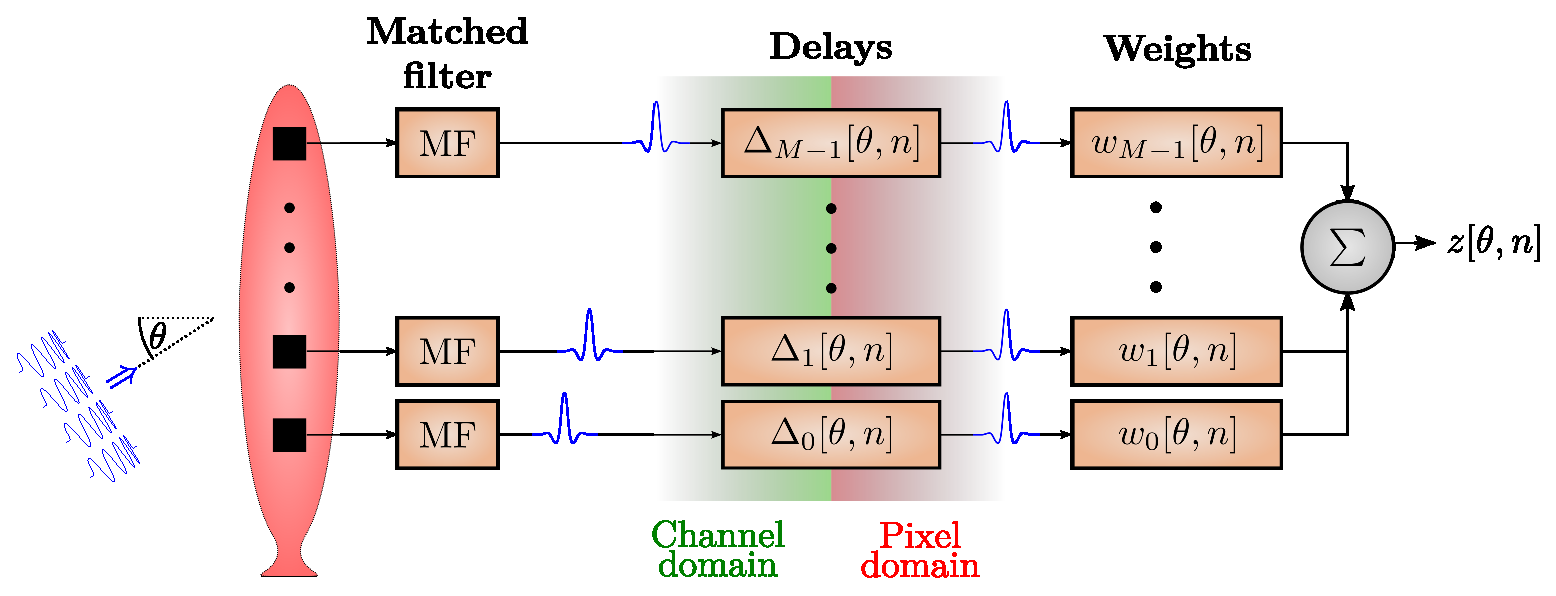
\includegraphics[width=\linewidth]{gfx/beamforming.eps}
\fi%
\caption{Beamforming principle. Signal signature is first removed by matched filtering. Then, before summation, a suitable set of delays $\Delta$ and weights $w$ are applied to focus on a pixel of interest at angle and range ($\theta,n$).}\label{beamforming}
\end{figure}
Let the receiver be an $M$ element uniform linear array, and assume that the signature of the transmitted signal has been removed by a matched filter (Fig. \ref{beamforming}). Further assume that the array channels are digitally delayed to focus at a pixel with azimuth angle $\theta$ and range sample $n$, such that the delayed data from the $m$th channel can be expressed as $x_m[\theta,n]$. To simplify notation, we make the dependence on $\theta$ implicit from now on. 

By definition, the beamformer output $z[n]$ can now be expressed as the weighted sum of all the delayed data samples:
\begin{align}
z[n] = \w\H[n]\x[n] = \bmat{w_0[n]\\w_1[n]\\\vdots\\w_{M-1}[n]}^H \bmat{x_0[n]\\x_1[n]\\\vdots\\x_{M-1}[n]},\label{z}
\end{align}
where $w_m$ is the weight factor assigned to channel $m$. With static weights this would be referred to as the conventional delay-and-sum (DAS) beamformer. A large variety of weighting functions exists here for trading lateral resolution for improved noise suppression (contrast), but one always ends up with a compromise between the two~\cite{Harris1978}.

Various adaptive beamformers target this limitation by allowing the weights to change for each pixel to better fit the dynamic nature of the incoming wavefield. In other words, they attempt to use the \emph{a priori} information present in the data to improve image quality. The MVDR beamformer is one such method. It finds the set of complex weights that minimizes the beamformer's expected output power, while ensuring unity gain in the look direction~\cite{Capon1969}. This is a convex optimization problem that can be solved using Lagrange multipliers to yield the solution
\begin{gather}
\vec w[n] = \frac{\Ri[n]\a}{\a\T\Ri[n]\a},\label{weights}
\end{gather}
where $\a$ is a steering vector and $\R=E\{\x[n]\x\H[n]\}\in\mathbb{C}^{M,M}$ is the spatial covariance matrix for the full array. Since we pre-steer our data to every pixel in the image we simplify (\ref{weights}) by substituting $\a$ with a row vector $\1$ that represents broadside phase-steering. To estimate $\R$ we compute a sample covariance matrix $\eR$. In this computation we perform some degree of:
\begin{itemize}
\item \emph{spatial averaging} to avoid signal cancellation by decorrelating coherent echoes~\cite{Kailath1985};
\item \emph{temporal averaging} over an interval comparable to the pulse length (one to five samples) to maintain true speckle statistics~\cite{Synnevag2009a};
\item \emph{diagonal loading} to improve robustness to parameter errors~\cite{Cox1987,Maksym1979}.
\end{itemize}%
%
% will perform some degree of \emph{spatial averaging} to avoid signal cancellation caused by coherent echoes~\cite{Kailath1985}, \emph{temporal averaging} to maintain true speckle statistics~\cite{Synnevag2009a}, and \emph{diagonal loading} to improve robustness to parameter errors ~\cite{Cox1987,Maksym1979}. 
%
Combined, these steps will also ensure a numerically well conditioned $\eR$.

We perform \emph{temporal} and \emph{spatial averaging} first and put the result in an intermediate sample covariance matrix $\breve{\R}$. To do this we need to segment our array into subarrays. If we let $x_l[n]$ represent the data vector from subarray $l$ by
\begin{gather}
\x_l[n] = \bmat{x_l[n] & x_{l+1}[n] & \dots & x_{l+L-1}[n]}\T,
\end{gather}
then $\breve{\R}$ can be calculated as
\begin{gather}
\breve{\R}[n] =  \frac{1}{N_K N_L} \sumb{l=0}{M-L}\sumb{n'=n-K}{n+K} \x_l[n']\x_l\H[n'] \in\mathbb{C}^{L,L},\label{spatialR}
\end{gather}
where $N_K = 2K+1$ is the number of temporal samples to perform averaging over, and $N_L = M-L+1$ is the number of subarrays.

The final estimate $\eR$ is found by adding a fraction $d$ of the total power of $\breve{\R}[n]$ to its diagonal~\cite{Synnevag2007}:
\begin{align}
\eR[n] = \breve{\R}[n] + \I \frac{d}{L} \tr\{\breve{\R}[n]\},\label{finalR}
\end{align}
where $\I$ is an identity matrix, $\tr\{\cdot\}$ represents the matrix trace operation, and $\tr\{\breve{\R}[n]\}$ is an estimate of the energy received from this pixel.

Note how subarray averaging led to a size reduction of $\eR$ from $\mathbb{C}^{M,M}$ to $\mathbb{C}^{L,L}$, and hence will produce an $L$-element weight set when substituted into (\ref{z}). This weight set is applied to all the subarrays, before computing the beamformer output as in (\ref{z}). Or, equivalently, we may apply the weight set to the sum of all the subarrays by
\begin{align}
z[n] = \w\H[n] \sumb{l=0}{M-L} \x_l[n].\label{finalZ}
\end{align}
\ifPeerReview
\begin{figure}[!t]\centering
\includegraphics[width=.8\linewidth]{gfx/buske2\figPostfix.eps}
\else
\begin{figure}[!t]\centering
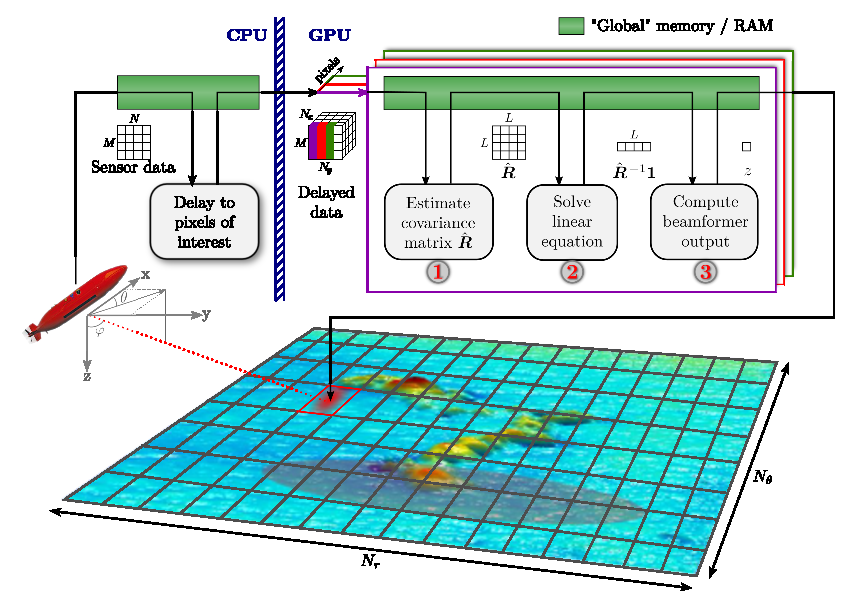
\includegraphics[width=\linewidth]{gfx/implementation.eps}
\fi%
\caption{MVDR beamforming. For each pixel in range and azimuth:\newline
1. an $L\times{}L$ sample covariance matrix $\eR$ is computed; \newline
2. the term $\eR^{-1}\1$ is found using a linear equation solver;\newline
3. and the beamformer output $z$ is computed from (\ref{finalZ}), where $\w$ is found by substituting $\eR^{-1}\1$ into (\ref{weights}). } \label{mvdr_beamforming}
\end{figure}
As summarized in Fig. \ref{mvdr_beamforming}, the MVDR method is applied to each pixel independently, by:
\begin{enumerate}
\item computing the sample covariance matrix $\eR$ in (\ref{finalR});
\item computing $\eRi\1$ in (\ref{weights});
\item computing the beamformer output $z$ in (\ref{finalZ}).
\end{enumerate}
Next we will evaluate these steps in terms of arithmetic complexity, and then discuss their mappability to parallel hardware.

\subsection{Computational Complexity}

 
% Computing and inverting $\eR$ is by far the most computationally intensive tasks in MVDR beamforming. This 

If we neglect spatial and temporal averaging, then the computation of $\eR$ is reduced to a single outer product with complexity of O($M^2$), and the inversion is then of O($M^3$). This might lead us to believe that the inversion step is by far the most complex. But if we implement spatial and temporal averaging as in (\ref{spatialR}), then computing $\eR$ is of O($N_K N_L L^2$) and the inversion of O($L^3$). Computing $\eR$ is now the most complex operation whenever $N_LN_K>L$.
\ifPeerReview
\begin{figure}[!t]\centering
\includegraphics[width=.8\linewidth]{gfx/buske3\figPostfix.eps}
\else
\begin{figure}[!t]\centering
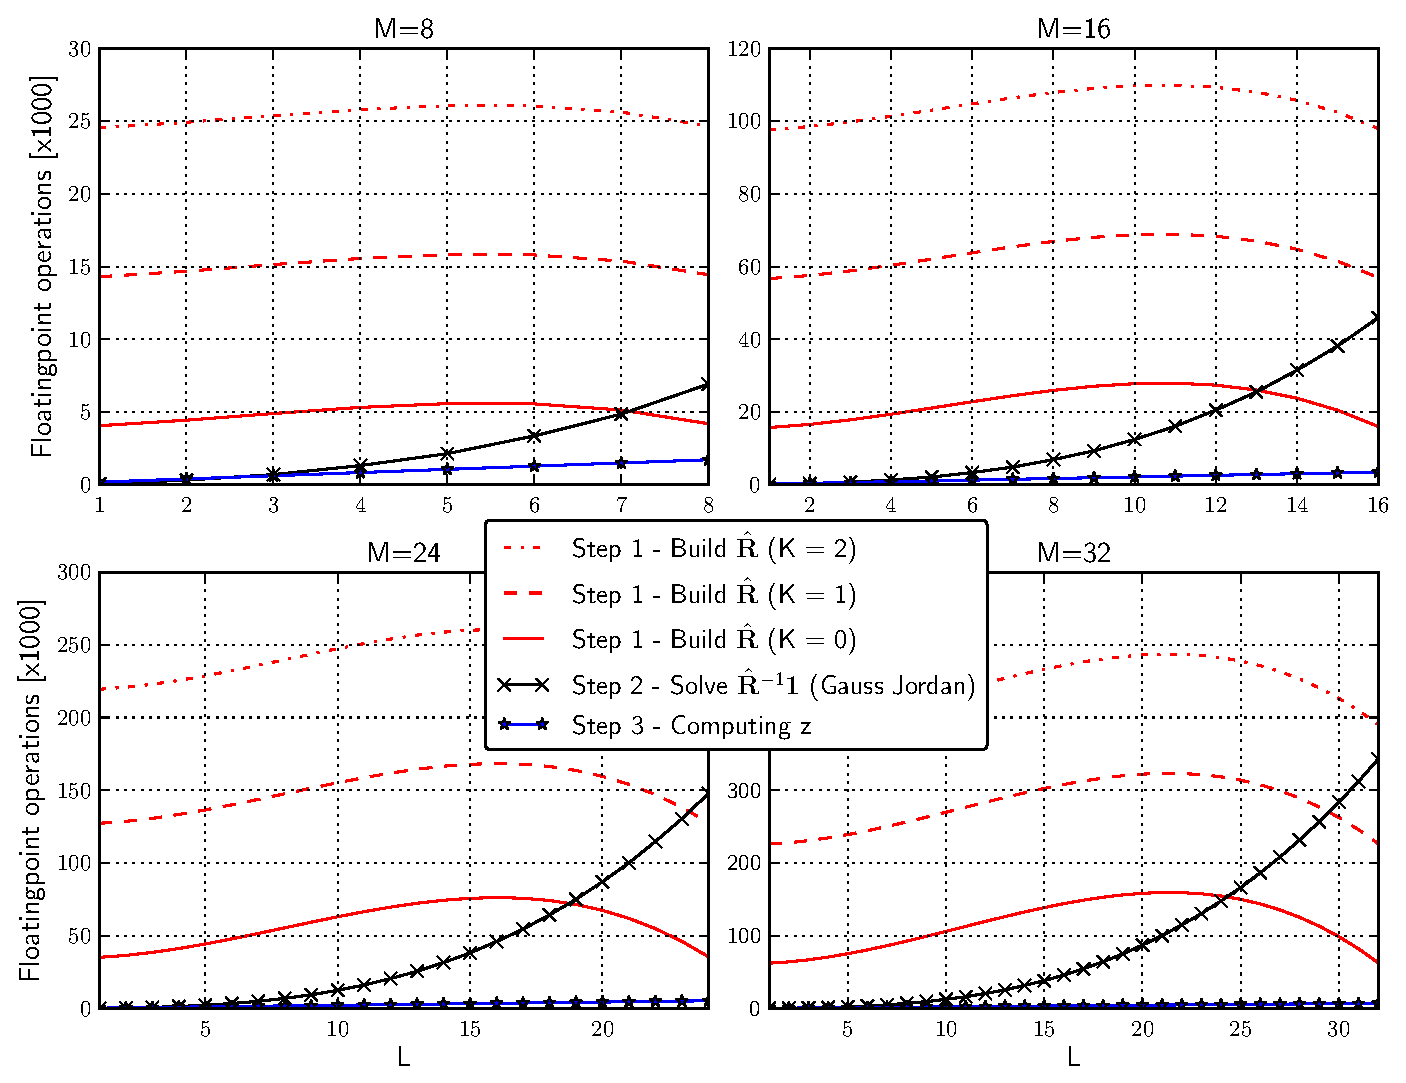
\includegraphics[width=\linewidth]{gfx/mvdr_complexity.eps}
\fi%
\caption{Per-pixel computational complexity of the steps in MVDR beamforming (before any optimizations). To avoid signal cancellation in an active sonar system we usually set $L<\frac{M}{2}$, in which region the computation of $\eR$ dominates in terms of arithmetic complexity, especially when performing temporal averaging.}\label{mvdr_complexity}
\end{figure}
To visualize these relations, and include the effects of using complex numbers, we set up complexity formulas that account for the total number of arithmetic operations for each step in the MVDR process (see appendix \ref{mvdr_formulas}). The only excluded operation was partial pivoting used in the inversion step, but this should contribute marginally to the end result. The entire range of possible subarray sizes from $L\in[1,M]$ was finally evaluated, with temporal averaging set to $K\in\{0,1,2\}$, and the number of channels set to $M\in\{8,16,32\}$. The results are shown in \Fig{mvdr_complexity}.

Note how the computation of $\eR$ completely dominates at smaller subarray sizes, that solving $\eRi\1$ only plays a notable role for larger array and subarray sizes, and that the computation of $z$ has a negligible impact on computation time. Also notice how temporal averaging comes with a high computational penalty. This is because building $\eR$ is heavy on complex multiplications, which require three times as many arithmetic instructions as a complex addition, and a lot of these are repeated unnecessarily.




\section{Mapping the MVDR to a GPU}\label{maptogpu}


An important feature of MVDR beamforming, as with beamforming in general, is that each pixel can be computed independently and in an identical fashion. Furthermore, a typical sonar image may contain millions of pixels. This represents a level of data parallelism that appears very well suited for a massively parallel architecture such as the GPU.

We decided to investigate the feasibility of running MVDR on a GPU by mapping it to a Nvidia GeForce Quadro 6000, which performs similarly to the consumer grade Geforce GTX 480. This is a high-end Compute Unified Device Architecture (CUDA)-enabled GPU based on Nvidia's Fermi architecture, which as now been superseded by the Kepler architecture. The code was written in Nvidia's ``C for CUDA'' framework, which adds a few extra features to the C language to specify how to distribute work across a large number of threads. It would have been possible to use GPUs from AMD and the cross-platform OpenCL framework from the Khronos group instead, but CUDA has a batch linear equation solver~\cite{Nvidia} that no OpenCL library provides. As will be discussed later, this is a key component in our design.

To use Nvidia's own terminology, the Quadro 6000 comprises 14 streaming multiprocessors (SMs), each having 32 CUDA cores that execute a common program called a kernel. Combined these cores deliver a peak performance of more than 1\;Tflop/s (appendix \ref{throughput}). In practice this performance is hard to obtain, but one can get fairly close by balancing the load evenly on all cores, and by trying to avoid that some cores are forced to idle due to a pending data transfer or thread synchronization. As the steps in the MVDR method require different strategies for achieving this, we have designed a different kernel and configuration for each of them. We will pay particular attention to building $\eR$, since the potential for gaining overall speedups are greatest here.

%  this assumes that the implementation is solely bound by arithmetic throughput.  r bound by memory bandwidth, arithmetic latency or arithmetic bandwidth.  or  is solely bound by processing power.   These cores need to be kept busy if we are to That make for a total of 448 CUDA cores which we need to keep busy if we want to tap the full potential. 

\ifPeerReview
\begin{figure}[t]\centering
\includegraphics[width=.8\linewidth]{gfx/buske4\figPostfix.eps}
\else
\begin{figure}[t]\centering
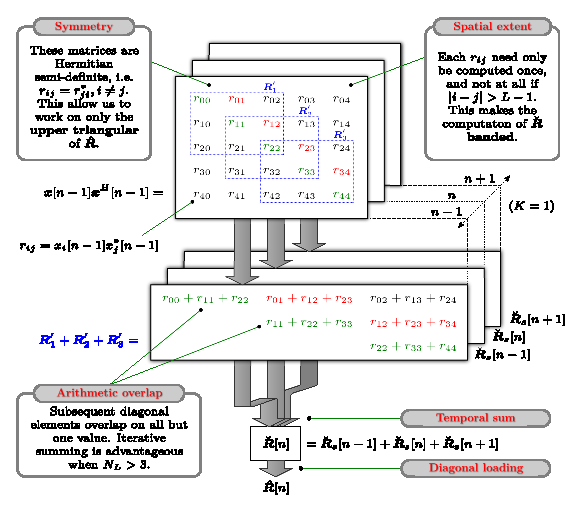
\includegraphics[width=\linewidth]{gfx/mvdr_build_R.eps}
\fi%
\caption{Step 1: Building $\eR$. This is a visualization of how $\eR$ could be built in a case with $M=5$ sensors, with subarray size $L=3$ and temporal averaging set to $K=1$. Here $\R'_{l}$ is the sample covariance matrix for the $l$th subarray, and $\breve{\R}$ is the average of $N_K$ of these. Note that instead of performing the temporal sum last as here, one could take more temporal samples into consideration in the computation of each $r_{ij}$.}\label{mvdr_build_R}
\end{figure}


% Memory latency can be hidden in two ways. One is to keep a lot of threads queued up on each SM at all times, such that when some threads perform memory operations other threads can be scheduled to run instead. This is referred to as data level parallelism (DLP). Alternatively, or preferrably in addition, the designer may promote instruction level parallelism (ILP) by letting subsequent instructions in a thread be independent. While ILP can be very effective when done correctly, DLP is generally simpler to design for.

% load balancing
% - distribute load - optimize symmetry
% - avoid branching
% 
% memory latency hiding
% - make threads use high bandwidth memory
% - hide latency with dlp, ilp, or both
% 
% thread sync hiding
% - queue blocks up on an sm

%This is referred to as a single-program, multiple-data (SPMD) architecture\todo{malplaced}.

 %An SM is a single-program multiple-data (SPMD) processor, meaning that all the CUDA cores on an instruction unit, L1 cache and registers is shared by all the CUDA cores on that SM.  %
% GPUs, on the other hand, does not attempt to do ILP, but use all available transistors to support massive DLP. This leads to designs such as the nNvidia GeForce GTX 580. 
% each with 48kB of L1 cache (shared memory) and 128kB of register memory.

% -bank conflicts when L > 32. not treated.


\subsection{Computing the Spatial Covariance Matrix, $\hat{\boldsymbol{R}}$}\label{computing_eR}

% As Fig. \ref{mvdr_complexity} illustrates the computation of $\eR$ 

As observed in Fig. \ref{mvdr_complexity}, a direct computation of $\eR$ by implementing (\ref{spatialR}) and (\ref{finalR}) is the greatest computational burden. We target this issue by first minimizing arithmetic operations, then aim to get as close to the peak arithmetic throughput on the GPU as possible.

\subsubsection{Minimizing Arithmetic Operations}

In Fig. \ref{mvdr_build_R}, we illustrate how to reduce the arithmetic complexity of building $\eR$ in a system with $M=5$ sensors, a subarray size of $L=3$, and temporal averaging is set to $K=1$. Here the spatial sum is carried out before the temporal sum. To reduce arithmetic operations we may:
%
\begin{enumerate}
\item exploit the fact that $\eR$ is Hermitian positive semidefinite to compute only one half of it;
\item avoid redundant multiplications;
\item avoid redundant summations by first computing the upper row of $\eR$ and then adding/subtracting to these iteratively to find the diagonals of $\eR$.
\end{enumerate}
%
\ifPeerReview
\begin{figure}[!t]\centering
\includegraphics[width=.8\linewidth]{gfx/buske5\figPostfix.eps}
\else
\begin{figure}[!t]\centering
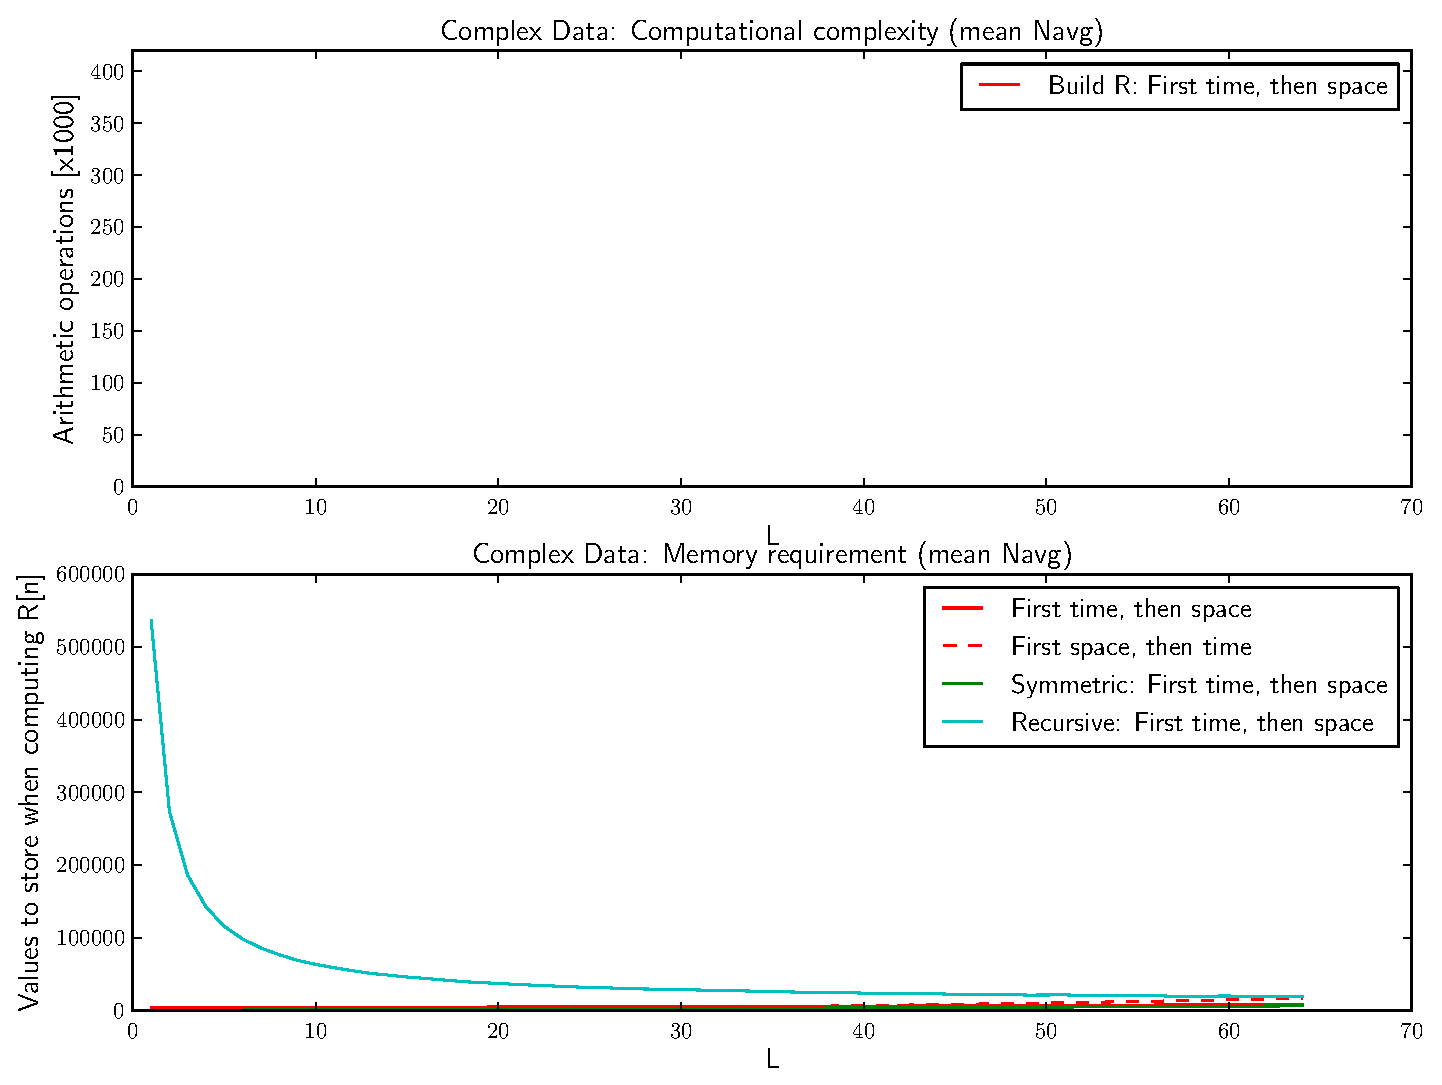
\includegraphics[width=\linewidth]{gfx/buildR-breakdown.eps}
\fi%
\caption{Arithmetic optimization of computing $\eR$: Relative reduction in arithmetic complexity compared to the initial implementation shown in Fig. \ref{mvdr_complexity} (higher is better) . Note how the arithmetic count is reduced by a factor 4-10 in the memory-optimized case, and by a factor 6-22 in the instruction-optimized case.}\label{mvdr_complexity_optimized}
\end{figure}

To study the effect of these optimizations we altered the complexity formulas to take them into account. Exploiting symmetry and performing iterative summing (step 1 and 3) is always desirable, but avoiding redundant multiplications (step 2) comes at the cost of increased memory consumption. When all optimizations are applied, we call it a "minimum instructions" solution, and when step 2 is left out, we call it a "minimum memory" solution. Fig. \ref{mvdr_complexity_optimized} compares the two solutions, and formulas may be found in Appendix \ref{mvdr_formulas}. Here the complexity curves are relative to the reference implementation in Fig. \ref{mvdr_complexity}. Both solutions reduce the complexity considerably, and recomputing the multiplications does not make that much of a difference. We selected the memory minimized version since our algorithm is severely memory bound, as we will see next.

\ifPeerReview
\begin{figure}[!t]\centering
\includegraphics[width=.8\linewidth]{gfx/buske6\figPostfix.eps}
\else
\begin{figure}[!t]\centering
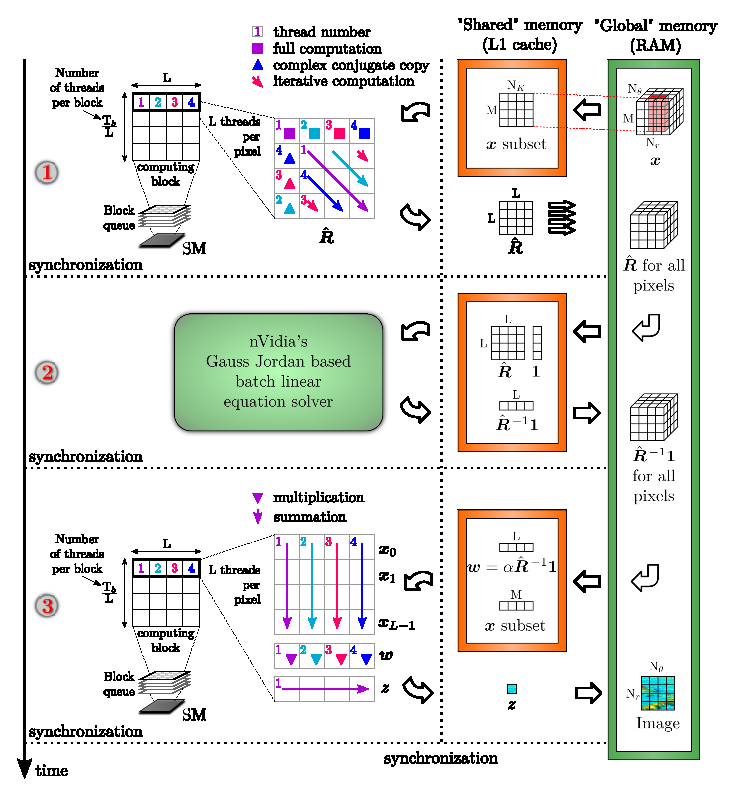
\includegraphics[width=\linewidth]{gfx/mvdr_implementation.eps}
\fi%
\caption{MVDR implementated on a GPU. We do this in 3 steps, where each step process the full image before moving on to the next step. \emph{Step~1}: The sample covariance matrix $\eR$ is formed by threads running along its diagonals. This allows spatial averaging to be implemented in a computationally efficient manner and minimizes interthread communication. \emph{Step~2}: $\eRi\1$ is computed using the heavily optimized batched linear equation solver from Nvidia~\cite{Nvidia}. \emph{Step~3}: The beamformer output $z$ is computed in a straightforward fashion using $L$ threads that first sum the subarrays and then apply the MVDR weighting function. A single thread finally sums all the channels up.}\label{mvdr_implementation}
\end{figure}

\subsubsection{Arithmetic Throughput}

When we compute $\eR$, we very rarely perform more than 1-3 floating point operations for every float read or written to memory. Unfortunately, the GPU prefers kernels to be more arithmetically intensive than this. This can be inferred from Table \ref{throughputs}, %
%
\begin{table}[!b]\centering%\normalsize
\begin{tabular}[c]{l r r r@{}  l}\hline
\rowcolor{tabBlue} & \multicolumn{1}{>{\columncolor{tabBlue}}c}{\bf B$_\text{arith}$} & \multicolumn{1}{>{\columncolor{tabBlue}}c}{\bf B$_\text{mem}$} & \multicolumn{2}{>{\columncolor{tabBlue}}c}{\bf B$_\text{mem}$/B$_\text{arith}$} \\\hline
Arithmetic & 1.03 Tflop/s & & &\\
Global memory & & 36 Gfloats/s & \hspace{30pt} 1 &:30 \\
Shared memory & & 257 Gfloats/s & 1 &:4 \\
Registers & & $>$1.5 Tfloats/s & $>$3 &:2~\cite{Vasilyy}
\end{tabular}
\caption{Nvidia Quadro 6000: Memory throughput, $B_{\lowercase{\text{mem}}}$, compared to arithmetic throughput, $B_\text{arith}$.}\label{throughputs}
\end{table}%
%
where the peak bandwidth of the three types of GPU memory are compared to the peak arithmetic throughput (see appendix \ref{throughput} for derivations). Global memory (RAM), in which all data must reside at some point, is at best only able to move one float for every 30 floats processed by the CUDA cores, and potentially much worse if care is not taken to use "coalesced" memory access patterns (that avoid memory bank conflicts). This is why the usage of global memory should be minimized. Shared memory, on the other hand, is a very fast level 1 cache that is shared by all threads on an SM. At peak performance, it is almost able to keep up with the computing units, but to obtain this performance we must make sure that:
\begin{enumerate}
\item the data needed to compute a pixel can fit in shared memory, while
\item the access patterns we use promote maximum bandwidth.
\end{enumerate}
 %Further alleviation is also possible by exposing instruction level parallelism within a thread, as this promotes the use of registers with a bandwidth at least 6 times higher than that of shared memory~\cite{Vasilyy}\todo{so why don't we? rephrase}.


These challenges are very closely linked. Since the Quadro 6000 architecture is of compute capability 2.0, it has 48\;kB shared memory (L1 cache) and 128\;kB of register memory per streaming multiprocessor (SM)~\cite{Nvidia2012}. This memory is shared by all active threads on that SM, a number that should be no less than 768~\cite{Nvidia2012a}. This is to expose a sufficient level of data parallelism to ensure that memory latency is completely hidden (in accordance with Little's law). If we divide the shared memory evenly on all 768 threads we find that each thread should store no more than 8 single precision complex numbers in shared memory, and 24 stored in registers. This should make it apparent why computing a single pixel per thread is a bad idea, and why we need to keep each thread as light on memory consumption as possible.

In Fig. \ref{mvdr_implementation}, we illustrate how we get around these challenges. First we make each SM compute entire range lines of pixels, then load the subset of $\x$ that all these pixels depend upon into shared memory. This lets us perform temporal averaging without having to read additional channel data.

Second, we assign $L$ threads per pixel to traverse the diagonals of $\eR$. On the top row, a full computation is carried out, then that row is saved back to global memory following a coalesced access pattern that maximizes global memory bandwidth. For subsequent rows, the threads move along the diagonals while performing iterative summations; the result from the previous element on the diagonal is updated by adding and subtracting the correlation coefficients that enter and exit the sum, respectively. To minimize memory consumption, we compute the coefficients again every time we need them. When a thread has finished up a diagonal, we have them wrap around to compute one of the diagonals in the lower triangular of $\eR$. Since $\eR$ is conjugate symmetric, the values in the leftmost column are obtained by a complex conjugate copy of the relevant value in the first row. This is slightly nonoptimal as it causes divergent branching, but it is needed because the solver is Gauss Jordan based and thus require a full $\eR$. Combined these steps balance the load evenly on all threads, is almost completely free of arithmetic redundancy, and cause little memory consumption.
 

% \cite{Owens2007}\todo{Find a good spot for these}

\subsection{Solving $\hat{\boldsymbol{R}}$$\;\!^{-1}$$\mathbf{1}$}

As intuition might suggest the matrix product $\eRi\1$ can be carried out by first inverting the matrix $\eR$, then performing the inner product with $\1$. However, one can also solve the linear equation $\hat{\boldsymbol{R}}\boldsymbol{b} = \1$ for $\boldsymbol{b}$, where $\boldsymbol{b} = \eRi\1$. This is the preferred approach since the solution is obtained directly and without the added computational cost of the final inner product.

An important thing to note here is that unlike the problems most GPU libraries try to solve, we do not attempt so solve large linear equations or invert large matrices; our matrices are small, but we have a very large number of them. Fortunately, Nvidia recently released a highly optimized batched linear equation solver tailored for this particular task. It is Gauss Jordan based and supports partial pivoting and complex numbers. The only downside to using it in our application is that it does not exploit the Hermitian property of our sample covariance matrix. A better choice would be a solver based on Cholesky decomposition. These are designed for Hermitian positive-semidefinite matrices such as our covariance matrix, and require only half the arithmetic operations of a Gauss Jordan solver.



\subsection{Computing $z$}

The beamformer output $z$ is computed on a per-pixel basis by first computing the MVDR weights $\w$, which are merely scaled versions of $\eRi\1$ (\ref{weights}). Then the sum in (\ref{finalZ}) is found by assigning a group of $L$ threads to respective elements of $x_l$, which then proceed to accumulate these for all $N_L$ subarrays. The resulting data vector is finally multiplied with the weight vector using the same threads, and then a single thread is used to sum these products to obtain $z$.

\subsection{Implementation summary}

% The GPU implementation can be summarized as follows:
% \begin{itemize}
% \item Pixels are processed in batches.
% \item Multiple threads per pixel.
% \item $\eR$ is computed directly from raw data to minimize memory footprint.
% \item Inversion step is performed by Nvidias batch linear equation solver.
% \item Design makes efficient use of cache and data transfers are kept to a minimum.
% \end{itemize}
% 
% We compare this to our CPU implementations, where:
% \begin{itemize}
% \item Pixels are processed one by one.
% \item Single thread per pixel.
% \item Computation of $\eR$ is optimized for minumum number of instructions, as in \ref{mvdr_build_R}. Only upper half of $\eR$ is computed (see next point).
% \item Inversion step carried out by a custom inline Cholesky based solver that only requires the upper triangular of $\eR$.
% \item Design has generally not been optimized for efficient use of memory.
% \end{itemize}

The GPU design is summarized and compared to our CPU designs in table \ref{implementation_summary}.
\begin{table}[!h]\centering%\normalsize
% \begin{tabular}[c]{l r r r@{}  l}\hline
\begin{tabular}[l]{l >{\raggedright}p{.27\linewidth} p{.28\linewidth}}\hline
\rowcolor{tabBlue} & \bf GPU & \bf CPU \\\hline
Pixel processing & In batches & One by one \\
Threads per pixel & Multiple & One \\
1. Building $\eR$:  & & \\
\ \ \ Values computed & All & Only upper triangular \\
\ \ \ Optimization    & Minimized memory consumption & Minimized number of instructions \\
2. Computing $\eRi\1$: & & \\
\ \ \ Method & Nvidia's batch\newline Gauss Jordan solver & Custom inline\newline Cholesky solver \\
Cache utilization & Efficient & Not efficient \\
Data transfers & Minimum & Moderate
\end{tabular}
\caption{Implementation summary.}\label{implementation_summary}
\end{table}


% There are essentially two ways to accelerate an algorithm on parallel hardware. One is to identify independent instructions for each thread, and run these in in parallel, and the other is to support the parallel execution of as many threads as possible. This is referred to as instruction level parallelism (ILP) and data level parallelism (DLP), respectively. Most general purpose processors, such as a CPUs, support both DLP by featuring multiple cores with single-data multiple-data (SIMD) capabilities, and ILP by through means such as branch prediction and out-of-order execution.

% GPUs, on the other hand, does not attempt to do ILP, but use all available transistors to support massive DLP. This leads to designs such as the nNvidia GeForce GTX 580. Using their own terminology, it is comprised of 16 ``streaming'' multiprocessors (SMs), each having having 32 CUDA\todo{make sure CUDA is introduced} cores that execute a common program called a kernel. %An SM is a single-program multiple-data (SPMD) processor, meaning that all the CUDA cores on an instruction unit, L1 cache and registers is shared by all the CUDA cores on that SM.  %
% each with 48kB of L1 cache (shared memory) and 128kB of register memory.




\section{Images and Benchmarks}\label{images_and_benchmarks}

To demonstrate the imaging capability of the MVDR beamformer, we have processed experimental datasets from the $M=32$ element Kongsberg Maritime HISAS1030 sonar mounted on a HUGIN autonomous underwater vehicle (AUV)~\cite{Hansen2009}. HISAS1030 is a high resolution synthetic aperture sonar (SAS) with an array length of 1.2\;m, operating frequency of 100\;kHz, and bandwidth of 30\;kHz. The element size and spacing is 2.5\;$\lambda$ and the opening angle is 25$^\circ$. To produce the image shown in \Fig{holmengraa}, the sonar was operated in sidescan mode. The studied object is the 1500-dwt oil tanker wreck Holmengraa. It is 68\;m long and 9\;m wide, and lies at a slanted seabed at 77\;m depth outside Horten, Norway. The 1 megapixel (MP) MVDR image was here processed with parameters $L=16$, $K=1$, and $d=1\%$.

\ifPeerReview
\begin{figure}[!t]\centering
\includegraphics[width=.8\linewidth]{gfx/buske7\figPostfix.eps}
\else
\begin{figure}[!t]\centering
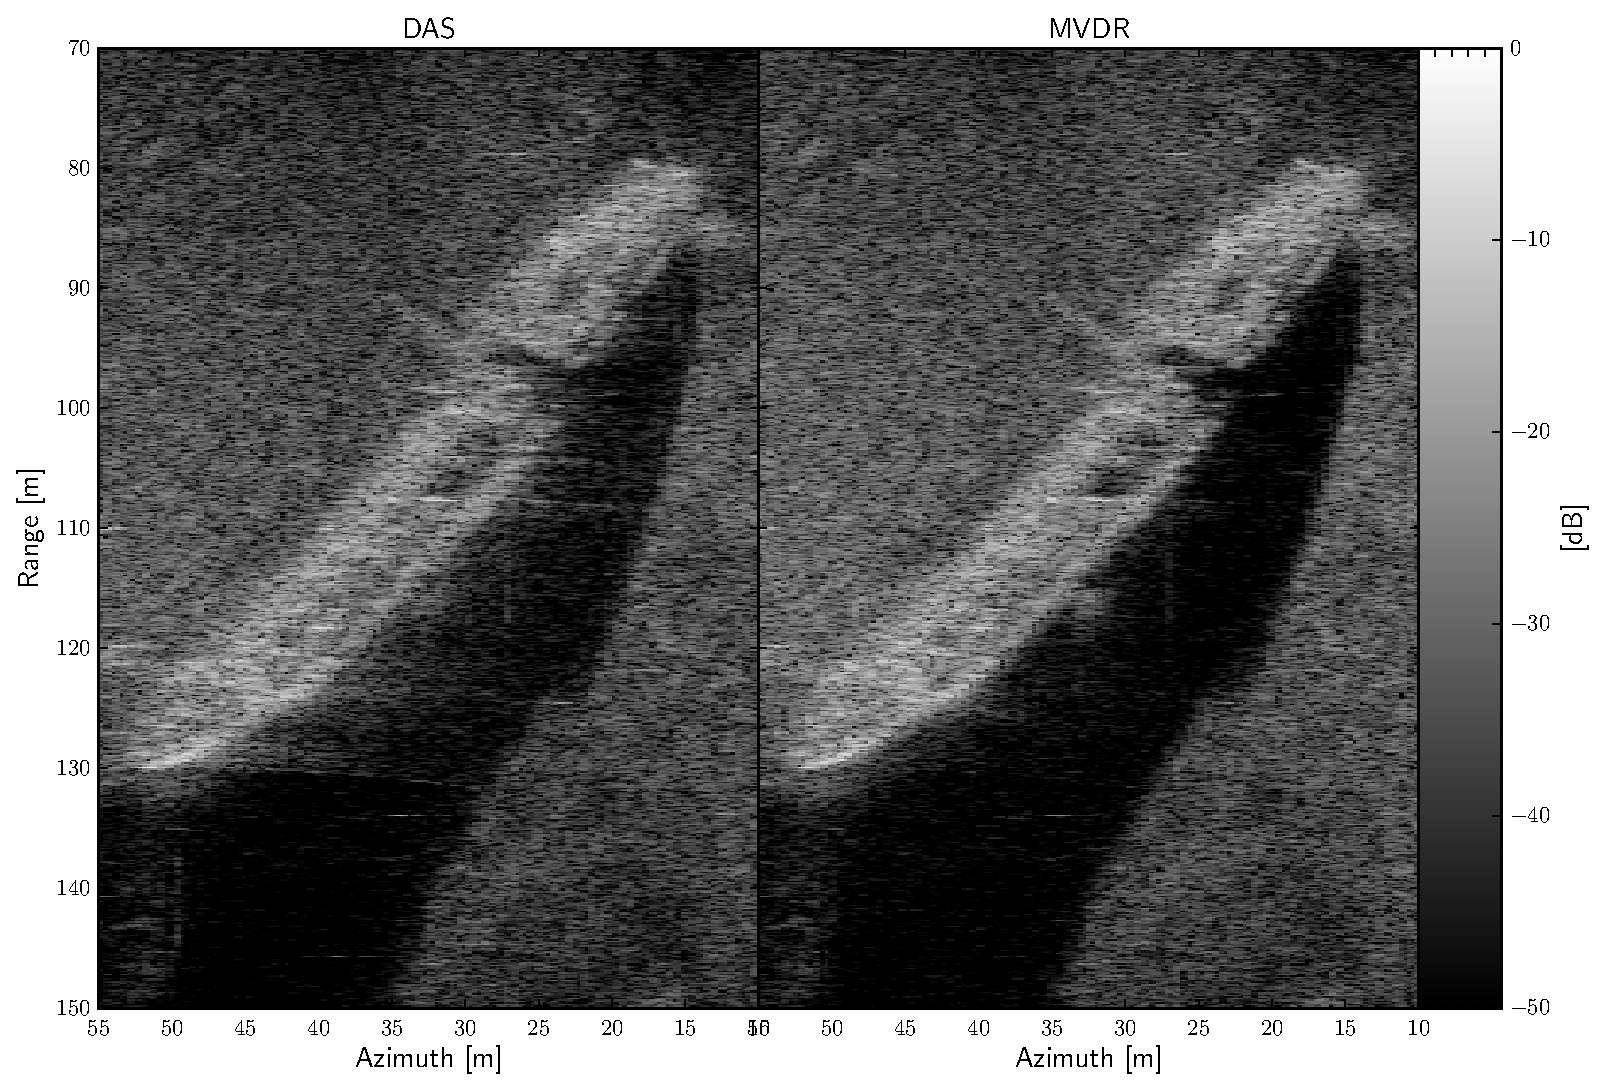
\includegraphics[width=\linewidth]{gfx/plot_holmengraa_L16_Navg1.eps}
\fi%
\caption{HISAS sidescan sonar (SSS) image of the shipwreck Holmengraa that lies on a slanted seabed at 77\;m depth outside of Horten, Norway. The image was processed with $M=32$, $L=16$, $K=1$ and $d=1\%$. The image was linearly upinterpolated by a factor 2 in azimuth making its total size 1.46 megapixels (MP). Note how MVDR improves edge definition and reduces noise in shadow regions.}\label{holmengraa}
\end{figure}

The computational performance of our implementation was first assessed on a test system with a quad-core Intel Xeon E5620, 64\;GB of RAM and an Nvidia Quadro 6000 card. The results were obtained by processing a 1\;MP image from the data from a 32 channel array, for all subarray sizes $L$, and for $K\in\{0,1,2\}$. Runtime measurements are shown in \Fig{benchmarks}. The runtimes of memory-only and arithmetic-only GPU kernels are depicted in \Fig{code_assessment}. An estimate of computation efficiency is presented in \Fig{code_assess_flops}. We were also granted a test drive at the Boston HPC centre on a machine with an Intel Xeon E5-2670, 32\;GB RAM and an Nvidia K20. The results from this run are shown in \Fig{benchmarks_boston}.

\ifPeerReview
\begin{figure}[!t]\centering
\includegraphics[width=.8\linewidth]{gfx/buske8\figPostfix.eps}
\else
\begin{figure}[!t]\centering
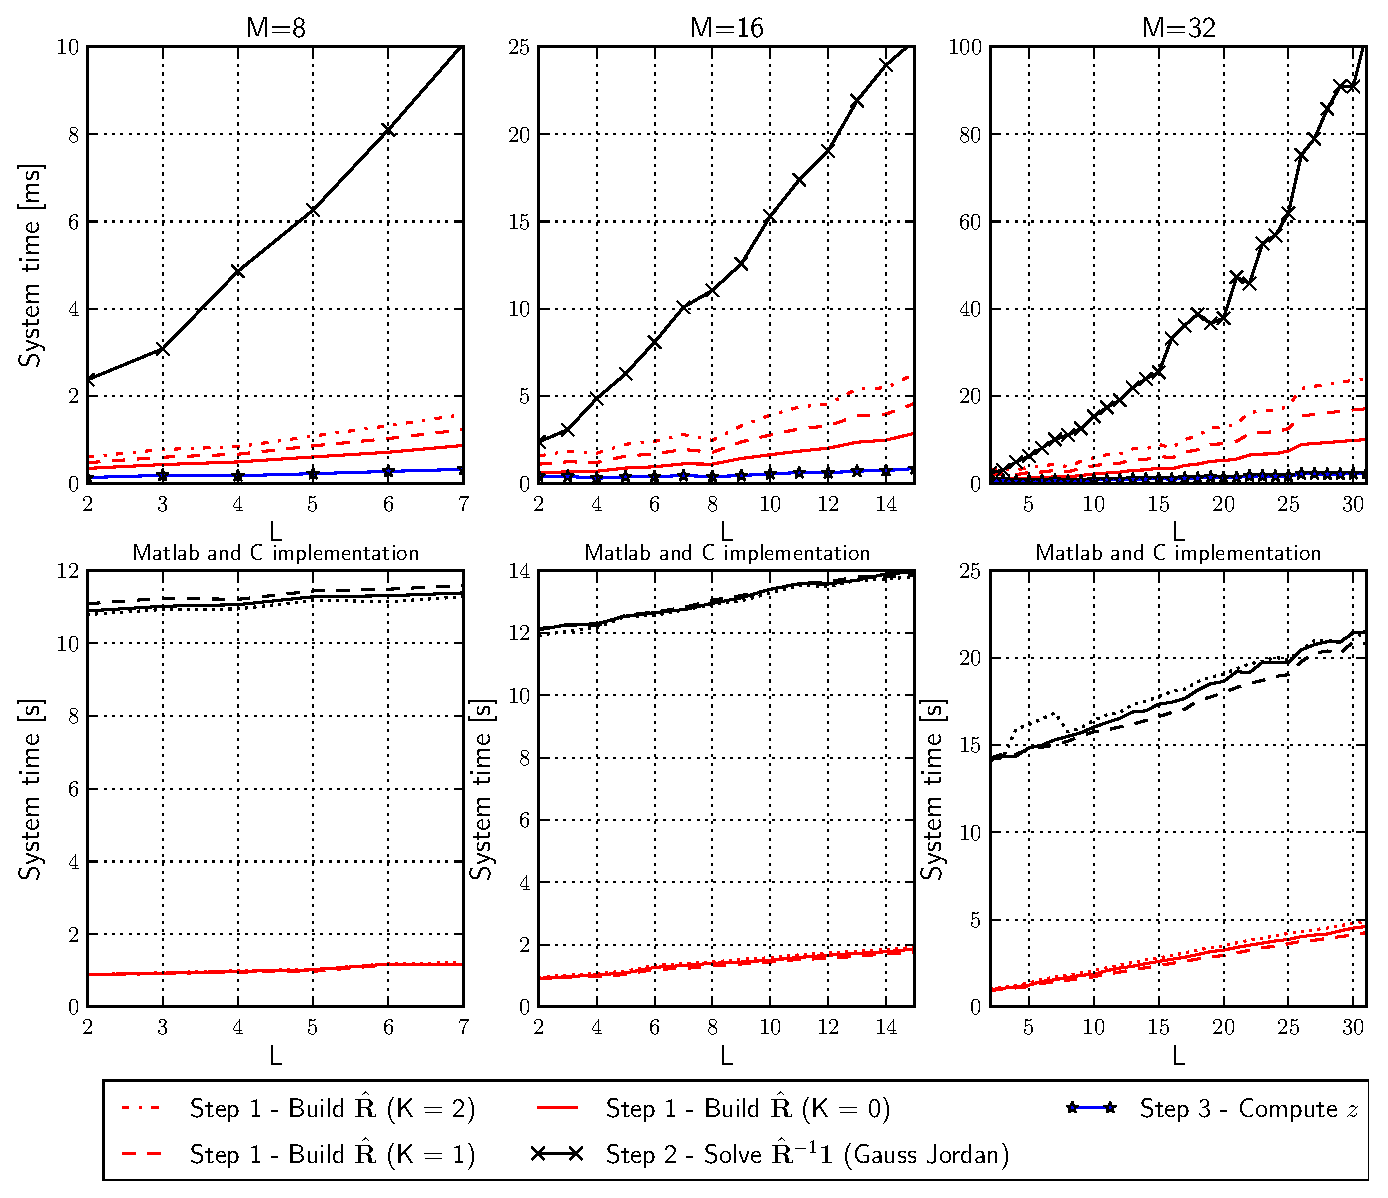
\includegraphics[width=\linewidth]{gfx/benchmark.eps}
\fi%
\caption{\protect MVDR benchmarks. A 1\;MP image from a $M=32$ channel array was processed for all $L$, and for $K\in\{0,1,2\}$.\newline \emph{Top:} The time the GPU spent on building $\eR$, solving $\eRi\1$, and computing $z$. Note the major speedup of building $\eR$ when compared to the complexity plot in Fig. \ref{mvdr_complexity}.\newline
\emph{Bottom:} Compared to a reference MATLAB and single thread C implementation running on a CPU the GPU offered a speedup of 2-3 orders of magnitude, but these numbers are somewhat misleading. If the C implementation was properly optimized we expect the GPU to be no more than a factor 5-10 faster, even if its theoretical peak performance is ~20 times higher than that of the CPU.}\label{benchmarks}
\end{figure}

\ifPeerReview
\begin{figure}[!t]\centering
\includegraphics[width=.8\linewidth]{gfx/buske9\figPostfix.eps}
\else
\begin{figure}[!t]\centering
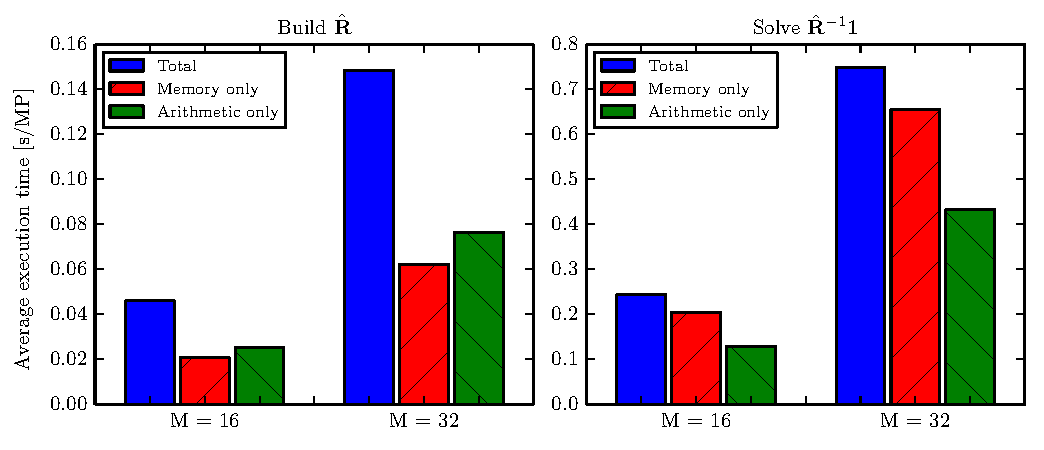
\includegraphics[width=\linewidth]{gfx/code_assessment.eps}
\fi%
\caption{Execution time of an arithmetic-only and a memory-only version of the MVDR code. A dataset from an $M=32$ array was processed for all $L$ using $K=1$, and the mean execution time for a 1 megapixel (MP) image was used here. From this plot we can infer that the kernel building $\eR$ is memory bound, as the time the kernel spends performing memory transactions is higher than the corresponding time it spends carrying out arithmetical operations. Furthermore, when the total runtime is larger than the restricted kernels this can largely be attributed to latency, which we can see that building $\eR$ suffers from with the chosen parameters.}\label{code_assessment}
\end{figure}

\ifPeerReview
\begin{figure}[!t]\centering
\includegraphics[width=.8\linewidth]{gfx/buske10\figPostfix.eps}
\else
\begin{figure}[!t]\centering
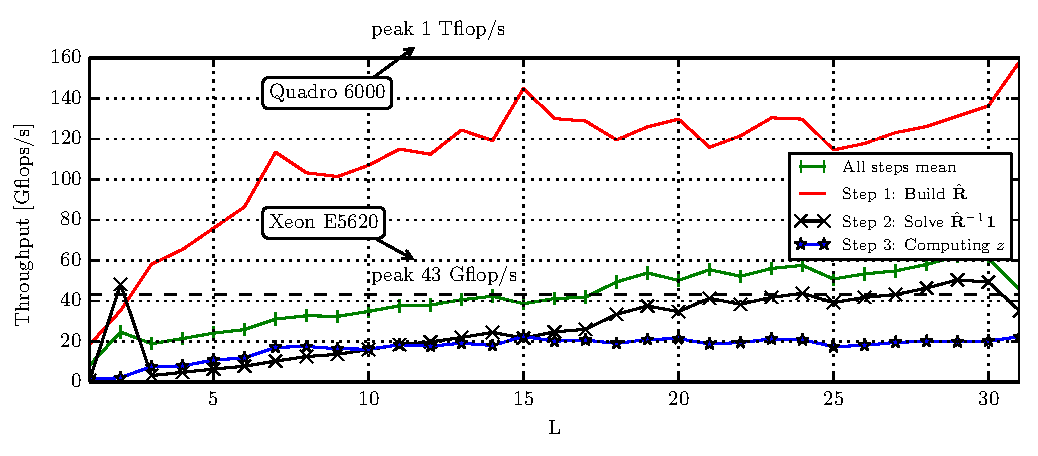
\includegraphics[width=\linewidth]{gfx/code_assess_flops.eps}
\fi
\caption{\protect Code efficiency. An estimate of the number of floating point operations per second (Flop/s), found by dividing the theoretical complexity curves by actual run-times. This is a crude measure as it does not include any other instructions than the actual arithmetic operations in the MVDR computation.}\label{code_assess_flops}
\end{figure}

\ifPeerReview
\begin{figure}[!t]\centering
\includegraphics[width=.8\linewidth]{gfx/buske11\figPostfix.eps}
\else
\begin{figure}[!t]\centering
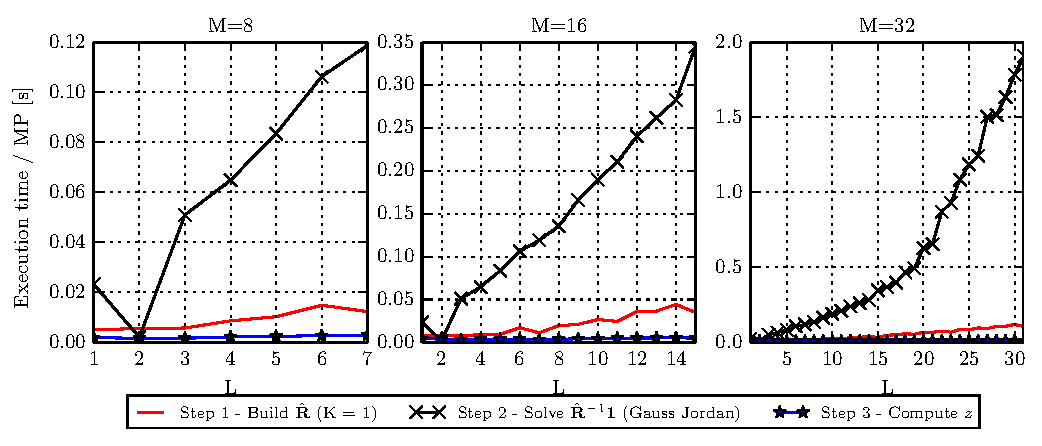
\includegraphics[width=\linewidth]{gfx/benchmark_boston.eps}
\fi
\caption{\protect MVDR benchmarks from Boston HPC centre with the new high-end Nvidia K20 Kepler GPU. The exact same scenario and code as in Fig. \ref{benchmarks} was used here. With no code alterations the performance was only improved marginally compared to running on the Quadro 6000.}\label{benchmarks_boston}
\end{figure}

As seen in the runtime comparisons presented in \Fig{benchmarks}, the GPU method became two to three orders of magnitude faster than the C implementation we started out with. The remaining bottleneck in the final design is the inversion step, which is typically five times slower than the build step. In most cases the processing speed of the Quadro 6000 is above 1\;MP/s, and this was only improved by a factor 1.5-2 when run on the new K20 GPU. The benchmarks of our memory-only and arithmetic-only kernels show that the kernels spend roughly the same time on both these tasks, so optimising only one of these further will have marginal impact. All GPU kernels were compiled with \texttt{nvcc} at optimization level \texttt{O2}. Excluded from these benchmarks is the data transfer time from CPU to GPU, which account for 2-20\% of the total processing time. We believe it makes little sense to include them since it keeps getting easier to perform these data transfers in parallel by offloading the task to the direct memory access (DMA) controllers present on modern GPUs. Furthermore, the data rates in an active sonar are relatively low compared to the bandwidth available for these transfers.


\section{Discussion}\label{discussion}

In accordance with previous studies, \Fig{holmengraa} demonstrates the MVDR beamformer's ability to produce images with suppressed interference and improved detail resolution. Compared to the DAS beamformer, the ship's edges appear sharper and the shadows less noisy. In this scenario the MVDR's performance was not particularly sensitive to parameter adjustments. Similar performance was obtained with arbitrary combinations of $L\in\{12,16,24\}$, $K\in\{1,2,3\}$ and $d\in[0.01,0.05]$, and no adjustments had to be made when processing other parts of the scene.

As observed in \Fig{benchmarks}, the combination of minimizing arithmetic operations and implementing the MVDR on a GPU lead to a significant improvement in processing speed. Compared to a MATLAB and single thread C implementation, an order 2 and 3 speedup was achieved, respectively. Note that we do not consider this comparison fair. In fact, the theoretical peak throughput of this GPU is roughly 20 times higher than that the CPU in question, meaning the potential of the CPU was far from being reached in our initial implementations. The key reason for this is that the GPU design processes pixels in batches, which allows us to minimize data transfers and maximize the use of fast memory cache. In other aspects the designs are similar, both CPU implementations compute $\eR$ efficiently, and they make use of either an optimized custom Cholesky based solver or one from the Intel Math Kernel Library (MKL). Unfortunately we had little time to write a custom batch based solver and covariance builder for the CPU, but we expect the speed difference to be five to ten times, if we had compared two such designs.

Note from \Fig{benchmarks} how the building of $\eR$ now only takes up a fraction of the total processing time, and recall that it was the other way around when we presented the theoretical complexity curves in \Fig{mvdr_complexity}. Also, the benchmark curves for building $\eR$ now seem linear. The main reason for this is that the optimization step negated much of the extra complexity introduced by averaging, i.e., reduced the complexity from O($N_KN_LL^2$) to less than O($L^2$). Another reason for the runtime to appear more like O($L$) is likely that our design makes better use of the GPU's resources when there is more processing involved per pixel. The inversion step, on the other hand, gains less from being implemented on a GPU. This is because its nature is less data parallel. In particular, the back substitution step involved in its computation is mostly sequential. This difference can be observed in \Fig{mvdr_complexity}. Alternative solvers, such as one based on Cholesky decomposition that exploits the Hermitian property of $\eR$, can in theory reduce complexity by a factor two, but we question whether this result can be obtained in practice using a GPU. The CPU implementations perform Cholesky-based inversion, but this does not explain why the C and MATLAB implementation have a total runtime that is linearly dependent on $L$. We believe this happens because these implementations are dominated by the calculation of the covariance matrix and data movement, and not by the inversion step. 

When optimizing a GPU design it is important to know whether it is limited by memory bandwidth or arithmetical throughput. To measure this we made two versions of the MVDR kernel: One that only performs arithmetic operations, and one that only performs memory operations. Then, we benchmarked these kernels and compared their runtimes to the total runtime (\Fig{code_assessment}). A first thing to note is how these kernels seem equally occupied performing memory and arithmetic operations. This is a good sign, but since we consistently minimized memory consumption at the expense of some extra computations when building $\eR$ , we know it to be bound by memory bandwidth. It also has a problem with latency, which can be inferred from the total runtime being significantly higher than that of the two single-function kernels. Since the GPU hardware can carry out memory and arithmetic operations concurrently and independently, this gap indicates that the GPU sometimes does ``nothing''. In our case this is due to synchronization hold-ups when performing temporal averaging, which is carried out in a sequential manner.

Even with all our efforts we were only able to obtain processing rates of 40\;GFlop/s on average in the desirable range of subarray sizes (\Fig{mvdr_complexity}). This is mainly due to the inversion step, since for the most part we obtained more than 100\;GFlop/s when building $\eR$. While these numbers are slightly underestimated, they are regardless far away from the Quadro 6000's peak of 1\;TFlop/s. Again, we believe this is due to the design being bound by memory bandwidth. This belief is further supported by the test results from running the code on the new K20 Kepler card, where we saw a modest factor 1.5-2 speedup. Although the Kepler card peaks at 3.5-4\;Tflop/s, its shared memory bandwidth is only approximately twice that of the Quadro 6000, hence matches the observed speedup. However, it is likely that the Kepler card would perform better had we optimized our design for it. For scientific computing, the Kepler boards are considered more attractive, with the introduction of features such as kernels calling kernels, more registers, more shared memory, and better mechanisms for hiding or removing data transfers.


% If the HISAS1030 was attached to a platform moving at 1.8m/s, for which the maximum range is 250\;m~\cite{Hansen2010}, the pulse repetition frequency could be set to 3\;Hz. We could further assume a complex sampling frequency of 40\;kHz to accomodate the  HISAS1030's bandwidth of 30\;kHz, and beamform $M=32$ lateral beams. The throughput required for real-time processing of these images would then be 1\;MP/s. As we have seen, this is something our GPU implementation can handle if $L$ is not too large.\todo{droppe denne kanskje}%, leaving the \gls{CPU} free to take on other assignments.


% What may this performance be used for? Let us assume that the 32 element, 1.2\;m long HISAS1030 array is mounted on a platform moving at 1.8\;m/s. Then the pulse repetition frequency (PRF) could be set to 3\;Hz to ensure critical along-track sampling, 
% To illustrate what this performance might be used for, consider a moving platform travelling at 1.8\;m/s. 
% If the sonar system is Maximum range 
% There is a limit to the along-track sampli
% To avoid along track undersampling, the 

% HUGIN: 1.8m/s - range 250m \\
% fs = 100kHz*30\%*$\frac{4}{3}$ = 40kHz \\
% $N_{range px} = \frac{2\;250m}{1500m/s}40kHz = 13.3kpx$ \\
% $\times 32$ beams = 426kpx \\\\
% 
% PRF = $\frac{1500m/s}{2 250m} = 3Hz$ \\
% TP = 215px 3Hz = 1.28MP/s \\
% 4 arrays: 1.28MP/s * 4 = 5.12MP/s
% 
% 
% \begin{itemize}
% \item Need for speed: HUGIN 4 banks of 32 elements, can be processed faster than the ping repetition rate, with margins to spare.
% \end{itemize}


\section{Conclusion}\label{conclusion}

The MVDR beamformer is an algorithm capable of producing images with improved detail resolution and contrast compared to conventional DAS beamforming. The downside is its inherent need for robustification and the high computational complexity associated with estimating and inverting the spatial covariance matrix.

We have shown that for systems consisting of up to 32 channels the problem can be largely mitigated by building the covariance matrix in a clever way, and by making use of the massive computational power available in modern GPUs. We were able to improve upon the runtime of a single thread C-implementation by roughly two orders of magnitude. For most choices of parameters the GPU was able to create images at $\sim$1\;MP/s at an average data processing rate of $\sim$40\;GFlop/s. This is less than 5\% of the peak performance of the GPU, but we believe it to be near optimal given the constraints of memory bandwidth and the sequential nature of some parts of the MVDR implementation.

%  This performance is sufficient for computing properly sampled full-coverage sectorscan images from the HISAS1030 sonar in real-time.

All in all, the MVDR maps well to the GPU since the computations involved are independent on the pixel level, and partially also within each pixel. The GPU allows MVDR to be used in real-time processing of sonar data, and makes the MVDR a viable alternative to conventional methods in practical systems.


%%%%%%%%%%%%%%%%%%                              ~~~~~~~~~~~~~~~~~~~~~~~~~~~~~~~~~~~~~~~~~~~~~~~~~~
% DOCUMENT APPENDICES %
%%%%%%%%%%%%%%%%%%                              ~~~~~~~~~~~~~~~~~~~~~~~~~~~~~~~~~~~~~~~~~~~~~~~~~~


% \titleformat{<command>}[<shape>]{<format}{<label>}{<sep>}{<before>}[<after>]

% \titleformat{\section}[hang]{\bf}
% {\thesection.\enspace}%\thesubsubsection}%  {\footnotesize \enspace \emph{Sec.}  }
%    {0pt}{\MakeUppercase}[]
% \titlespacing*{\section}{0pt}{2\lineheight}{\lineheight}

% {-2ex plus -.5ex minus -.2ex}{1.0ex plus .2ex minus .2ex}

% \renewcommand\section[1]{{\Large\bf\MakeUppercase #1}}
% \renewcommand\section*[1]{{\Large\bf\MakeUppercase #1}}

% 
% 
% 
% 
% 
% 
% PRF = $\frac{1500m/s}{2 250m} = 3Hz$ \\
% TP = 215px 3Hz = 1.28MP/s \\
% 4 arrays: 1.28MP/s * 4 = 5.12MP/s
% 
% 
% 
% 1Tflops (ops/cycle?)
% 144GB/s global
% 1TB/s shared
% x6 regs
% 
% latency - arithmetic (20 cycles) and memory (400+ cycles)
% 
% Little's law - needed parallelism = latency * throughput
% arithmetic: 23 cycles * 32ops/SM/cycle = 576 ops/SM parallelism
% memory: <800 cycles * <144GB/s=125B/cycle = <100kB in the flight
% 
% On GF104: must have some ILP to get >0.66 of peak:
% - 48cores/SM, one instruction is broadcast across 16 cores
% - need 3 instructions per cycle
% - but only have 2 warp schedulers
% - instead, can issue 2 instructions per warp in the same cycle
% 

\appendices

\section{MVDR Complexity Formulas}\label{mvdr_formulas}

To estimate the number of floating point operations needed to MVDR beamform a single pixel, we formed expressions that accumulate the number of complex arithmetic operations found in the MVDR process. From observing the generated assembly code we inferred that each complex addition and multiplication would require $\Oa = 2$ and $\Om = 6$ floating point operations, respectively. The formulas are listed for each step below for reference.

\emph{Building $\eR$}. The initial complexity of this step can be inferred directly from (\ref{spatialR}) and (\ref{finalR}):
\begin{align}
O_{\underset{\text{initial}}{\text{Build $\eR$}}} &= \underbrace{\Om\Nk\Nl L^2}_\text{Multiplications} + \underbrace{\Oa(\Nk+\Nl-2)L^2}_\text{Additions} + O_\text{dload},
\end{align}
where $O_\text{dload} = (2L-1)\Oa + \Om$ is the minor cost of performing diagonal loading. If we apply the optimization strategies discussed in section \ref{computing_eR} we can arrive at the following instead:
\begin{align}
O_{\underset{\text{min arith}}{\text{Build $\eR$}}} &= \underbrace{\Om\frac{M+\Nl}{2}L}_\text{Multiplications} + \underbrace{\Oa(\Nk-1)(\Nl-1)L}_\text{First row additions} \nonumber\\
&+ \underbrace{\frac{(L-1)(L-2)}{2} \bigg[ 2\Oa + 2(\Nk-1)\Oa \Big]}_\text{Iteration additions} \nonumber\\
&+ O_\text{dload}
\end{align}
Of the solutions discussed, this is the least expensive in terms of arithmetic instructions. However, if memory bandwidth is a limiting factor a better solution is to recompute multiplications where they are needed:
\begin{align}
O_{\underset{\text{min mem}}{\text{Build $\eR$}}} &= \underbrace{\Om\Nk\Nl{}L}_\text{First row multiplications} + \underbrace{O_a(\Nk-1)(\Nl-1)L}_\text{First row additions} \nonumber\\
&+ \underbrace{\frac{(L-1)(L-2)}{2}\bigg[ 2\Oa + 2(\Nk-1)\Oa + 2\Nk\Om \bigg]}_\text{Iteration multiplications and additions} \nonumber\\
&+ O_\text{dload}.
\end{align}

\emph{Solving $\eRi\1$} is achieved by using a batched Gauss Jordan solver with support for complex numbers and partial pivoting. Its complexity, with partial pivoting excluded, can be expressed as: 
\begin{align}
O_{\text{Solve $\eRi\1$}} = \sumb{r=0}{L} \bigg[&\underbrace{\big(L-r\big)\big((L-r+2)\Oa + (L-r+3)\Om\big)}_\text{Reduction}\nonumber\\
+ &\underbrace{(r-1)\Oa + r\Om}_\text{Backsubstitution}\bigg],
\end{align}
where $r$ is a running variable $r$ that indexes rows in the augmented matrix $\bmat{\eR|\1}$.

\emph{Computing $z$} is very simple once the covariance matrix $\eR$ is built and inverted, and has an near negligible impact on performance: 
\begin{align}
O_\text{Compute $z$} = \Oa(2L-2)2 + \Om 3 L.
\end{align}



\section{GPU Throughput}\label{throughput}

In the context of determining whether an implementation is computationally bound or memory bound, one should first compare the target platform's sustained computational throughput to sustained memory throughput. Let us start with the former.

The Quadro 6000 has 32 CUDA cores per SM, each operating at a rate of 1148\;MHz and being able to perform 2 floating point operations (flop) per clock cycle when multiply-add instructions are used. The theoretical peak arithmetic throughput is then given as
\begin{align}
\text{B}_\text{arith} &= 2\cdot1148\;\text{Mflop/s/core}\cdot 32\;\text{cores/SM}\cdot 14\;\text{SMs}\nn
&= 1.03\;\text{Tflop/s}.\label{flops}
\end{align}
Now let us compare this to the memory throughput. The ``global'' GDDR5 memory bus is 384\;bit wide, and operates at 3\;Ghz where 2 bits are sent every cycle. Its peak bandwidth is then
\begin{align}
\text{B}_\text{gmem} &= \frac{2\cdot 3\;\text{Gbit/s}\cdot384\;\text{bit}}{8\;\text{bit/byte}}\nn
&= 144\;\text{GB/s}\ (36\;\text{Gfloats/s}).\label{bwglobal}
\end{align}
The shared memory, on the other hand, is organized into 32 banks per SM, each being 32\;bit wide and operating at 1148\;MHz where 1 bit is sent per cycle. Its peak aggregated bandwidth is then
\begin{align}
\text{B}_\text{smem} &= \frac{\frac{1148}{2}\;\text{Mbit/s}\cdot32\;\text{bit/bank}\cdot 32\;\text{banks/SM}\cdot 14\;\text{SMs}}{8\;\text{bit/byte}}\nn
&\approx 1.03\;\text{TB/s}\ (257\;\text{Gfloats/s}).\label{bwshared}
\end{align}
The bandwidths are compared in Tab. \ref{throughputs}. Note that even when using shared memory at least 4 floating point operations must be carried out per float transferred to the CUDA cores, otherwise the algorithm will be memory bound and the peak arithmetic throughput can not be reached.



%%%%%%%%%%%%%%%%%%                              ~~~~~~~~~~~~~~~~~~~~~~~~~~~~~~~~~~~~~~~~~~~~~~~~~~
% DOCUMENT APPENDICES %
%%%%%%%%%%%%%%%%%%                              ~~~~~~~~~~~~~~~~~~~~~~~~~~~~~~~~~~~~~~~~~~~~~~~~~~

\appendices

% use section* for acknowledgement
\ifCLASSOPTIONcompsoc% % This command fixes abstract positioning for compsoc articles:
% \IEEEdisplaynotcompsoctitleabstractindextext
% 
% % (Optional) Add some extra info on cover page of peer review papers:
% % \ifCLASSOPTIONpeerreview
% % \begin{center} \bfseries EDICS Category: 3-BBND \end{center}
% % \fi
% 
% % Insert page break and insert second title (peer review mode)
% \IEEEpeerreviewmaketitle
% 
% 
% 


  \section*{Acknowledgments}
\else
  \section*{Acknowledgment}
\fi


The authors would like to thank Kongsberg Maritime and the Norwegian Defence Research Establishment (FFI) for providing experimental data, and thank Nvidia for providing support on running the batched linear equation solver and for granting us a testdrive at the Boston HPC center.


% Can use something like this to put references on a page
% by themselves when using endfloat and the captionsoff option.
\ifCLASSOPTIONcaptionsoff
  \newpage
\fi


\bibliographystyle{IEEEtran}
\bibliography{library.bib}

% Generated by IEEEtran.bst, version: 1.13 (2008/09/30)
\begin{thebibliography}{10}
\def\url#1{}
\csname url@samestyle\endcsname
\providecommand{\newblock}{\relax}
\providecommand{\bibinfo}[2]{#2}
\providecommand{\BIBentrySTDinterwordspacing}{\spaceskip=0pt\relax}
\providecommand{\BIBentryALTinterwordstretchfactor}{4}
\providecommand{\BIBentryALTinterwordspacing}{\spaceskip=\fontdimen2\font plus
\BIBentryALTinterwordstretchfactor\fontdimen3\font minus
  \fontdimen4\font\relax}
\providecommand{\BIBforeignlanguage}[2]{{%
\expandafter\ifx\csname l@#1\endcsname\relax
\typeout{** WARNING: IEEEtran.bst: No hyphenation pattern has been}%
\typeout{** loaded for the language `#1'. Using the pattern for}%
\typeout{** the default language instead.}%
\else
\language=\csname l@#1\endcsname
\fi
#2}}
\providecommand{\BIBdecl}{\relax}
\BIBdecl

\bibitem{Benitz1997}
\BIBentryALTinterwordspacing
G.~R. Benitz, ``{High-Definition Vector Imaging},'' \emph{Lincoln Laboratory
  Journal}, vol.~10, no.~2, pp. 147--170, 1997.
  \url{http://www.ll.mit.edu/publications/journal/journalarchives10-2.html}
\BIBentrySTDinterwordspacing

\bibitem{Synnevag2007}
\BIBentryALTinterwordspacing
J.-F. Synnev\aa{}g, A.~Austeng, and S.~Holm, ``{Adaptive beamforming applied to
  medical ultrasound imaging.}'' \emph{IEEE transactions on ultrasonics,
  ferroelectrics, and frequency control}, vol.~54, no.~8, pp. 1606--13, Aug.
  2007.  \url{http://www.ncbi.nlm.nih.gov/pubmed/19811995}
\BIBentrySTDinterwordspacing

\bibitem{Blomberg2012a}
\BIBentryALTinterwordspacing
A.~E.~A. Blomberg, A.~Austeng, and R.~E. Hansen, ``{Adaptive Beamforming
  Applied to a Cylindrical Sonar Array Using an Interpolated Array
  Transformation},'' \emph{IEEE Journal of Oceanic Engineering}, vol.~37,
  no.~1, pp. 25--34, Jan. 2012.
  \url{http://ieeexplore.ieee.org/lpdocs/epic03/wrapper.htm?arnumber=6112183}
\BIBentrySTDinterwordspacing

\bibitem{Blomberg2011}
A.~E.~A. Blomberg, R.~E. Hansen, S.~A.~V. Synnes, and A.~Austeng, ``{Improved
  interferometric sonar performance in shallow water using adaptive
  beamforming},'' in \emph{Proceedings of the International Conference \&
  Exhibition on Underwater Acoustic Measurements (UAM), Kos, Greece, June},
  2011.

\bibitem{Dursun2009}
S.~Dursun, A.~Austeng, R.~E. Hansen, and S.~Holm, ``{Minimum variance
  beamforming in active sonar imaging},'' in \emph{Proceedings of the 3rd
  International Conference \& Exhibition on Underwater Acoustic Measurements:
  Technologies and Results}, B.~e. {John S. Papadakis \& Leif}, Ed., 2009, pp.
  1373--1378.

\bibitem{Lo2004}
\BIBentryALTinterwordspacing
K.~Lo, ``{Adaptive Array Processing for Wide-Band Active Sonars},'' \emph{IEEE
  Journal of Oceanic Engineering}, vol.~29, no.~3, pp. 837--846, Jul. 2004.
  \url{http://ieeexplore.ieee.org/lpdocs/epic03/wrapper.htm?arnumber=1353435}
\BIBentrySTDinterwordspacing

\bibitem{Widrow1982}
\BIBentryALTinterwordspacing
B.~Widrow, K.~Duvall, R.~Gooch, and W.~Newman, ``{Signal cancellation phenomena
  in adaptive antennas: Causes and cures},'' \emph{IEEE Transactions on
  Antennas and Propagation}, vol.~30, no.~3, pp. 469--478, May 1982.
  \url{http://ieeexplore.ieee.org/lpdocs/epic03/wrapper.htm?arnumber=1142804}
\BIBentrySTDinterwordspacing

\bibitem{VanTrees2002}
\BIBentryALTinterwordspacing
H.~L. {Van Trees}, \emph{{Optimum Array Processing}}.\hskip 1em plus 0.5em
  minus 0.4em\relax New York, USA: John Wiley \& Sons, Inc., Mar. 2002.
  \url{http://doi.wiley.com/10.1002/0471221104}
\BIBentrySTDinterwordspacing

\bibitem{Kailath1985}
\BIBentryALTinterwordspacing
T.~Kailath and T.-J. Shan, ``{Adaptive beamforming for coherent signals and
  interference},'' \emph{IEEE Transactions on Acoustics, Speech, and Signal
  Processing}, vol.~33, no.~3, pp. 527--536, Jun. 1985.
  \url{http://ieeexplore.ieee.org/lpdocs/epic03/wrapper.htm?arnumber=1164583}
\BIBentrySTDinterwordspacing

\bibitem{Asl2012a}
\BIBentryALTinterwordspacing
B.~M. Asl and A.~Mahloojifar, ``{A low-complexity adaptive beamformer for
  ultrasound imaging using structured covariance matrix.}'' \emph{IEEE
  transactions on ultrasonics, ferroelectrics, and frequency control}, vol.~59,
  no.~4, pp. 660--7, Apr. 2012.
  \url{http://www.ncbi.nlm.nih.gov/pubmed/22547277}
\BIBentrySTDinterwordspacing

\bibitem{Jakobsson2000}
\BIBentryALTinterwordspacing
A.~Jakobsson, S.~Marple, and P.~Stoica, ``{Computationally efficient
  two-dimensional Capon spectrum analysis},'' \emph{IEEE Transactions on Signal
  Processing}, vol.~48, no.~9, pp. 2651--2661, 2000.
  \url{http://ieeexplore.ieee.org/lpdocs/epic03/wrapper.htm?arnumber=863072}
\BIBentrySTDinterwordspacing

\bibitem{Nilsen2009}
\BIBentryALTinterwordspacing
C.-I.~C. Nilsen and I.~Hafizovic, ``{Digital beamforming using a GPU},'' in
  \emph{2009 IEEE International Conference on Acoustics, Speech and Signal
  Processing}.\hskip 1em plus 0.5em minus 0.4em\relax IEEE, Apr. 2009, pp.
  609--612.
  \url{http://ieeexplore.ieee.org/lpdocs/epic03/wrapper.htm?arnumber=4959657}
\BIBentrySTDinterwordspacing

\bibitem{Chen2011}
\BIBentryALTinterwordspacing
J.~Chen, Y.~Yiu, and H.~So, ``{Real-time GPU-based adaptive beamformer for high
  quality ultrasound imaging},'' \emph{IEEE Ultrasonics Symposium}, vol.~1,
  no.~1, pp. 1--4, 2011.  \url{http://hub.hku.hk/handle/10722/140228}
\BIBentrySTDinterwordspacing

\bibitem{Chen2011a}
\BIBentryALTinterwordspacing
J.~Chen, B.~Y. Yiu, B.~K. Hamilton, A.~C. Yu, and H.~K.-H. So, ``{Design space
  exploration of adaptive beamforming acceleration for bedside and portable
  medical ultrasound imaging},'' \emph{ACM SIGARCH Computer Architecture News},
  vol.~39, no.~4, p.~20, Dec. 2011.
  \url{http://dl.acm.org/citation.cfm?doid=2082156.2082162}
\BIBentrySTDinterwordspacing

\bibitem{Chapman1976}
\BIBentryALTinterwordspacing
D.~Chapman, ``{Partial adaptivity for the large array},'' \emph{IEEE
  Transactions on Antennas and Propagation}, vol.~24, no.~5, pp. 685--696, Sep.
  1976.
  \url{http://ieeexplore.ieee.org/lpdocs/epic03/wrapper.htm?arnumber=1141408}
\BIBentrySTDinterwordspacing

\bibitem{Asen2012}
J.~P. \AA{}sen, J.~I. Buskenes, C.-I.~C. Nilsen, A.~Austeng, and S.~Holm,
  ``{Implementing Capon Beamforming on the GPU for Real Time Cardiac Ultrasound
  Imaging},'' in \emph{Proceedings IEEE Ultrasonics Symposium}, 2012.

\bibitem{Asen2013}
\BIBentryALTinterwordspacing
J.~P. \AA{}sen, J.~I. Buskenes, C.-I. {Colombo Nilsen}, A.~Austeng, and
  S.~Holm, ``{Implementing capon beamforming on a GPU for real-time cardiac
  ultrasound imaging.}'' \emph{IEEE transactions on ultrasonics,
  ferroelectrics, and frequency control}, vol.~61, no.~1, pp. 76--85, Jan.
  2014.  \url{http://www.ncbi.nlm.nih.gov/pubmed/24402897}
\BIBentrySTDinterwordspacing

\bibitem{Buskenes2013}
\BIBentryALTinterwordspacing
J.~I. Buskenes, J.~P. \AA{}sen, C.-I.~C. Nilsen, and A.~Austeng, ``{Adapting
  the minimum variance beamformer to a graphics processing unit for active
  sonar imaging systems},'' \emph{The Journal of the Acoustical Society of
  America}, vol. 133, no.~5, p. 3613, 2013.
  \url{http://link.aip.org/link/JASMAN/v133/i5/p3613/s2\&Agg=doi}
\BIBentrySTDinterwordspacing

\bibitem{Harris1978}
\BIBentryALTinterwordspacing
F.~Harris, ``{On the use of windows for harmonic analysis with the discrete
  Fourier transform},'' \emph{Proceedings of the IEEE}, vol.~66, no.~1, pp.
  51--83, 1978.
  \url{http://ieeexplore.ieee.org/lpdocs/epic03/wrapper.htm?arnumber=1455106}
\BIBentrySTDinterwordspacing

\bibitem{Capon1969}
\BIBentryALTinterwordspacing
J.~Capon, ``{High-resolution frequency-wavenumber spectrum analysis},''
  \emph{Proceedings of the IEEE}, vol.~57, no.~8, pp. 1408--1418, 1969.
  \url{http://ieeexplore.ieee.org/lpdocs/epic03/wrapper.htm?arnumber=1449208}
\BIBentrySTDinterwordspacing

\bibitem{Synnevag2009a}
\BIBentryALTinterwordspacing
J.-F. Synnev\aa{}g, A.~Austeng, and S.~Holm, ``{Benefits of minimum-variance
  beamforming in medical ultrasound imaging},'' \emph{IEEE Transactions on
  Ultrasonics, Ferroelectrics and Frequency Control}, vol.~56, no.~9, pp.
  1868--1879, Sep. 2009.
  \url{http://ieeexplore.ieee.org/lpdocs/epic03/wrapper.htm?arnumber=5278437}
\BIBentrySTDinterwordspacing

\bibitem{Cox1987}
\BIBentryALTinterwordspacing
H.~Cox, R.~Zeskind, and M.~Owen, ``{Robust adaptive beamforming},'' \emph{IEEE
  Transactions on Acoustics, Speech, and Signal Processing}, vol.~35, no.~10,
  pp. 1365--1376, Oct. 1987.
  \url{http://ieeexplore.ieee.org/lpdocs/epic03/wrapper.htm?arnumber=1165054}
\BIBentrySTDinterwordspacing

\bibitem{Maksym1979}
\BIBentryALTinterwordspacing
J.~N. Maksym, ``{A robust formulation of an optimum cross-spectral beamformer
  for line arrays},'' \emph{The Journal of the Acoustical Society of America},
  vol.~65, no.~4, p. 971, 1979.
  \url{http://link.aip.org/link/JASMAN/v65/i4/p971/s1\&Agg=doi}
\BIBentrySTDinterwordspacing

\bibitem{Nvidia}
\BIBentryALTinterwordspacing
Nvidia, ``{Nvidia registered developers program}.''
  \url{https://developer.nvidia.com/registered-developer-programs}
\BIBentrySTDinterwordspacing

\bibitem{Vasilyy}
\BIBentryALTinterwordspacing
V.~Volkov, ``{GTC: Better Performance at Lower Occupancy},'' 2010.
  \url{http://www.cs.berkeley.edu/~volkov/volkov10-GTC.pdf}
\BIBentrySTDinterwordspacing

\bibitem{Nvidia2012}
\BIBentryALTinterwordspacing
Nvidia, \emph{{CUDA C Programming Guide v4.2}}, 2012.
  \url{http://developer.nvidia.com/cuda/nvidia-gpu-computing-documentation}
\BIBentrySTDinterwordspacing

\bibitem{Nvidia2012a}
\BIBentryALTinterwordspacing
Nvidia, \emph{{CUDA C Best Practices Guide v4.1}}, 2012.
  \url{http://developer.nvidia.com/cuda/nvidia-gpu-computing-documentation}
\BIBentrySTDinterwordspacing

\bibitem{Hansen2009}
R.~E. Hansen, H.~J. Callow, T.~O. S\ae{}b\o, S.~A. Synnes, P.~E. Hagen,
  G.~Fossum, and B.~Langli, ``{Synthetic aperture sonar in challenging
  environments: Results from the HISAS 1030.}'' in \emph{Proceedings of the 3rd
  International Conference \& Exhibition on Underwater Acoustic Measurements:
  Technologies and Results}, 2009.

\end{thebibliography}



\begin{IEEEbiography}[{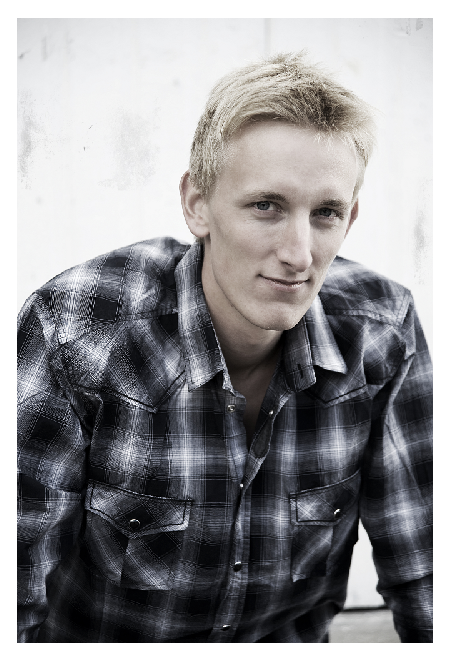
\includegraphics[width=1in,height=1.25in,clip,keepaspectratio]{bio/jo_inge.eps}}]{Jo Inge Buskenes}
received the B.Sc. degree in electrical engineering from Gj\o{}vik College University, Norway, in 2007, and the M.Sc. degree in instrumentation for particle physics from the University of Oslo, Norway, in 2010. He is currently pursuing the Ph.D. degree in image reconstruction and technology at the University of Oslo.

His industry experience includes the European Organization for Nuclear Research (CERN), Geneva, Switzerland (2007-2008), and the Norwegian Defence Research Establishment, Kjeller, Norway (2009). He has lectured in digital signal processing at the Gj\o{}vik College University (2009), and at the University of Oslo (2010-2012). His research interests include adaptive beamforming, digital image reconstruction, high performance computing, intelligent detector design and open source software.
\end{IEEEbiography}

\begin{IEEEbiography}[{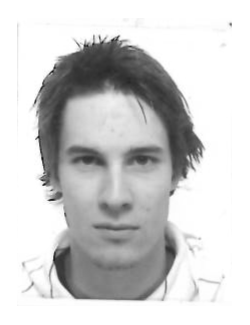
\includegraphics[width=1in,height=1.25in,clip,keepaspectratio]{bio/jon_petter.eps}}]{Jon Petter \AA{}sen}
(S'12) was born in Porsgrunn, Norway in 1986. He received the B.Sc. and M.Sc. degree in computer science from the University of Oslo, Norway, in 2010. He is currently pursuing his Ph.D. degree in medical ultrasound technology at the Norwegian University of Science and Technology (NTNU) Medical Imaging Lab (MI-Lab), Trondheim, Norway. His research interests include adaptive ultrasound processing techniques and acceleration of ultrasound algorithms using Graphics Processing Units (GPUs). 
\end{IEEEbiography}

\begin{IEEEbiography}[{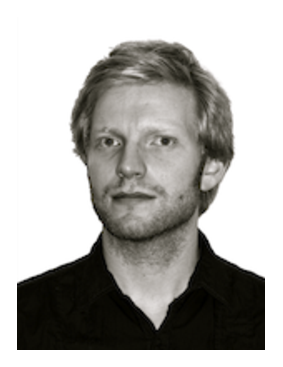
\includegraphics[width=1in,height=1.25in,clip,keepaspectratio]{bio/carl-inge.eps}}]{Carl-Inge Colombo Nilsen}
(S'06-M'10) received the M.Sc. and Ph.d. degrees in computer science from the University of Oslo, Norway, in 2005 and 2010. He is currently working at the University of Oslo as a postdoctoral research fellow. His research interests include signal and array processing for ultrasound imaging and other acoustical applications.
\end{IEEEbiography}

\begin{IEEEbiography}[{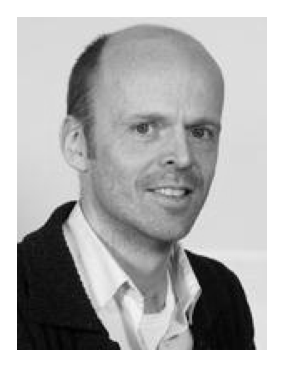
\includegraphics[width=1in,height=1.25in,clip,keepaspectratio]{bio/andreas.eps}}]{Andreas Austeng}
was born in Oslo, Norway, in 1970. He received the M.Sc. degree in physics in 1996 and the Ph.D. degree in computer science in 2001, both from the University of Oslo. Since 2001, he has been working at the Department of Informatics, University of Oslo, first as a postdoctoral research fellow and currently as an associate professor. His research interests include signal and array processing for acoustical imaging.
\end{IEEEbiography}


% 
% IMAGE METRICS
%
% - Point spread function (res via main lobe width, SAS gain via PDF height)
% - Constrast measures
%
% ACR = cL/2
% C = (s+n)/n ratio
% - 
% WHO's needing processing power
% - Centre for Maritime Research and Experimentation


\vfill 

\end{document}



}
\newpage\addcontentsline{toc}{section}{References}
\putbib[./Paper1/library]
\end{bibunit}

\setcounter{chapter}{1}

%%%% Paper 2 %%%%
\begin{bibunit}[IEEEtran]
\CustChapterPaper{Implementing Capon Beamforming on a GPU for Real-Time Cardiac Ultrasound Imaging}
\runningtitle{GPU Capon Beamformer for Cardiac Ultrasound Imaging}
\authors{
	\textbf{Jon Petter \AA{}sen}$^{1}$,
    	Jo Inge Buskenes$^{2}$,  
    	Carl-Inge C. Nilsen$^{2}$,
    	Andreas Austeng$^{2}$ and
    	Sverre Holm$^{1,2}$
} 
{
	$^{1}$Medical Imaging Lab (MI-Lab), Norwegian University of Science and Technology, Trondheim, Norway\\
    	$^{2}$Department of Informatics, University of Oslo, Oslo, Norway
}
\noindent \textit{IEEE Transactions on Ultrasonics, Ferroelectrics, and Frequency Control, vol. 61, pp. 76-85, Jan 2014}.
\newpage
{\input{./Paper2/cos}}
\newpage
\addcontentsline{toc}{section}{References}
\putbib[./Paper2/cosbib]
\end{bibunit}


%%%% Paper 3 %%%%
\begin{bibunit}[IEEEtran]
\CustChapterPaper{Capon Beamforming and Moving Objects - An Analysis of Lateral Shift-Invariance}
\runningtitle{Capon Beamforming and Moving Objects}
\authors{
	\textbf{Jon Petter \AA{}sen}$^{1}$, 
    	Andreas Austeng$^{2}$ and
    	Sverre Holm$^{1,2}$
} 
{
	$^{1}$Medical Imaging Lab (MI-Lab), Norwegian University of Science and Technology, Trondheim, Norway\\
    	$^{2}$Department of Informatics, University of Oslo, Oslo, Norway
}
\noindent \textit{IEEE Transactions on Ultrasonics, Ferroelectrics, and Frequency Control, , vol. 61, no. 7, pp. 1152-1160, Jul 2014}.
\newpage\input{./Paper3/moving_obj}
\newpage\addcontentsline{toc}{section}{References}
\putbib[./Paper3/moving_objbib]
\end{bibunit}


%%%% Paper 4 %%%%
\begin{bibunit}[IEEEtran]
\CustChapterPaper{Adaptive Volume Rendering of Cardiac 3D Ultrasound Images - Utilizing Blood Pool Statistics}
\runningtitle{Adaptive Volume Rendering of Cardiac Ultrasound}
\authors{
	\textbf{Jon Petter \AA{}sen}$^{1}$,
	Erik Steen$^2$,
	Gabriel Kiss$^{3,4}$,
	Anders Thorstensen$^{1,5}$,
	Stein Inge Rabben$^2$
}
{
$^{1}$Medical Imaging Lab (MI-Lab), Norwegian University of Science and Technology, Trondheim, Norway\\
$^{2}$ GE Vingmed Ultrasound, Horten, Norway\\
$^{3}$ Norwegian University of Science and Technology, ISB - Department of Circulation and Medical Imaging, Trondheim, Norway\\
$^{4}$ St. Olavs Hospital, Trondheim, Norway\\
$^{5}$ Department of Cardiology, St. Olavs Hospital, Trondheim, Norway
}
\noindent \textit{Proc. SPIE Medical Imaging 2012, vol. 8320, pp. 832008.}
\newpage%%%%%%%%%%%%%%%%%%%%%%%%%%%%%%%%%%%%%%%%%%%%%%%%%%%%%%%%%%%%% 
\begin{abstract}
In this paper we introduce and investigate an adaptive direct volume rendering (DVR) method for real-time visualization of cardiac 3D ultrasound.  DVR is commonly used in cardiac ultrasound to visualize interfaces between tissue and blood. However, this is particularly challenging with ultrasound images due to variability of the signal within tissue as well as variability of noise signal within the blood pool. Standard DVR involves a global mapping of sample values to opacity by an opacity transfer function (OTF). While a global OTF may represent the interface correctly in one part of the image, it may result in tissue dropouts, or even artificial interfaces within the blood pool in other parts of the image. In order to increase correctness of the rendered image, the presented method utilizes blood pool statistics to do regional adjustments of the OTF. The regional adaptive OTF was compared with a global OTF in a dataset of apical recordings from 18 subjects. For each recording, three renderings from standard views (apical 4-chamber (A4C), inverted A4C (IA4C) and mitral valve (MV)) were generated for both methods, and each rendering was tuned to the best visual appearance by a physician echocardiographer. For each rendering we measured the mean absolute error (MAE) between the rendering depth buffer and a validated left ventricular segmentation. The difference $d$ in MAE between the global and regional method was calculated and t-test results are reported with significant improvements for the regional adaptive method ($\bar{d}_{A4C} = 1.5 \pm 0.3$ mm, $\bar{d}_{IA4C} = 2.5 \pm 0.4$ mm, $\bar{d}_{MV} = 1.7 \pm 0.2$  mm, d.f. $= 17$, all $p<0.001$). This improvement by the regional adaptive method was confirmed through qualitative visual assessment by an experienced physician echocardiographer who concluded that the regional adaptive method produced rendered images with fewer tissue dropouts and less spurious structures inside the blood pool in the vast majority of the renderings. The algorithm has been implemented on a GPU,  running an average of 16 fps with a resolution of 512x512x100 samples (Nvidia GTX460).
\end{abstract}

\graphicspath{{./Paper4/img/}}

\section{Introduction}
Direct volume rendering (DVR)\cite{Levoy1988} is commonly used in cardiac ultrasound to visualize interfaces between tissue and blood\cite{steen1994, Rabben2010, kiss2010}. DVR has the advantage over other methods like 2D-slicing that it presents a large part of the volumetric data in a single view. Figure \ref{fig:dvr}a presents such a volume rendering of a high quality cardiac ultrasound volume. Anatomical structures of special interest are highlighted; the left ventricle (LV), the mitral valve which separates LV from the left atrium (LA), and the interventricular septum which separates the LV from the right ventricle (RV). As can be seen, interpreting cardiac ultrasound data is difficult and requires a lot of training. Clear tissue-blood boundaries are therefore of great importance. However, this is challenging to achieve with ultrasound images due to variability of the signal within tissue as well as variability of noise signal within the blood pool.
\begin{figure}  
\begin{center}
\begin{minipage}[b]{0.5\linewidth}\centering
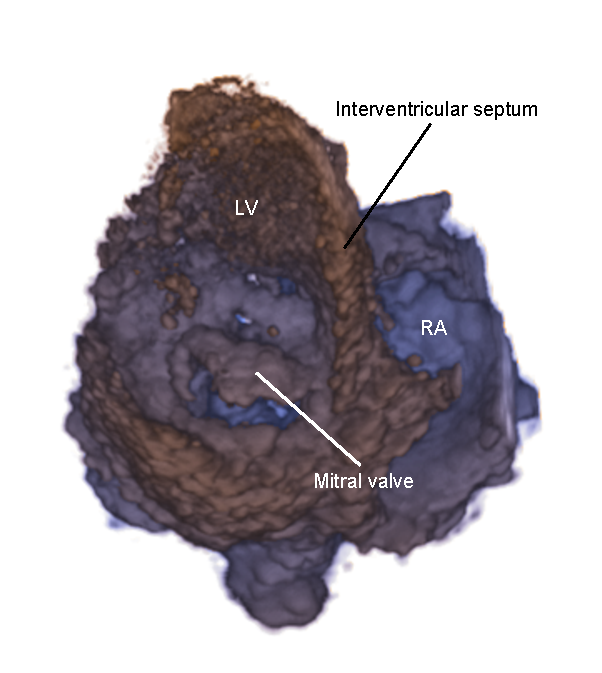
\includegraphics[height=1\textwidth]{vr_cardiac_high_quality.eps}\\
(a)
\end{minipage}%
\hspace{-5em}
\begin{minipage}[b]{0.6\linewidth}\centering
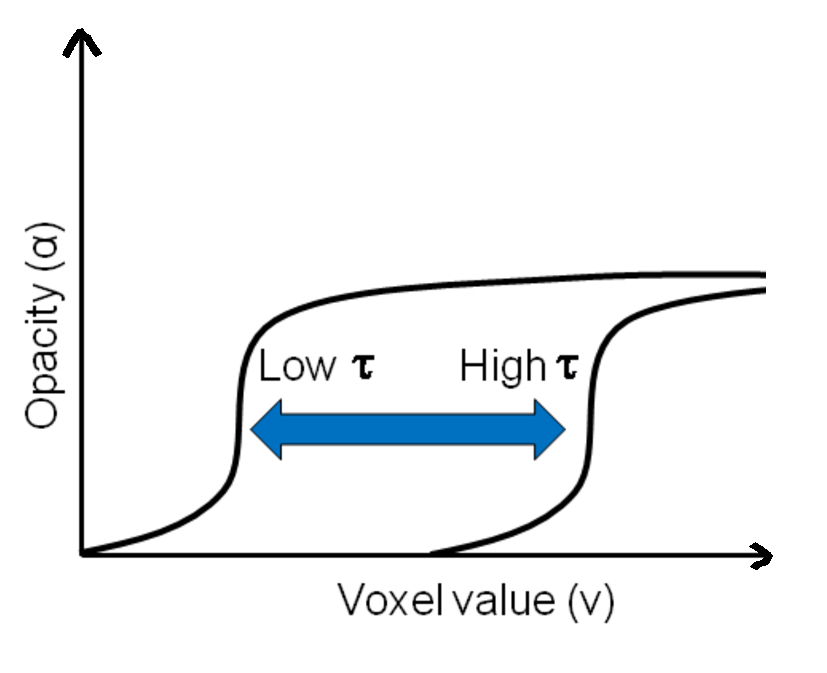
\includegraphics[height=0.4\textwidth]{otf2.eps}\\
(b)
\end{minipage} 
\end{center}
\caption[example] { \label{fig:dvr}  a). An example of direct volume rendering (DVR) of cardiac ultrasound. Highlighted anatomical structures are: The left ventricle (LV), the right atrium (RA), mitral valve and the interventricular septum.  b). Shows two opacity transfer functions (OTF) with a fuzzy transition between voxels excluded from (values below $\tau$) or included in the rendering (values above $\tau$). Adjusting $\tau$ (blue arrow) will either include or exclude more data.}
\end{figure} 
%DVR is based on a physical model of light moving through a gaseous medium, and for simplicity, only absorption and emission along each ray are considered in its standard formulation. 

At the core of DVR, optical properties (colour and opacity) are derived from a transfer function and integrated along rays of light. One ray for each pixel in the final image. Applying the transfer function is also known as classification since features are visually separated through assignment of different colours and opacities. On the other hand, selecting a transfer function with low classification error is considered a challenge and will always be related to the data at hand \cite{pfister2002transfer}. Figure \ref{fig:dvr}b shows an example of a monotonically increasing opacity transfer function (OTF) for cardiac ultrasound DVR. Unlike other medical imaging modalities like CT and MR, cardiac ultrasound data are assumed to consist of only two classes; tissue and the blood pool signal. Tissue is expected to have higher intensity than blood, but in practice the two class-distributions overlap. The OTF in Figure \ref{fig:dvr}b is therefore designed to give a fuzzy threshold between samples excluded from and samples included in the rendering. Selecting the right threshold, as for transfer functions design in general, is therefore a challenge in cardiac ultrasound visualization.   

There are several reasons for the overlap between tissue and blood pool signal in ultrasound images. Sidelobes of the ultrasound beam results in signal from off-beam structures (clutter noise). Speckle pattern, caused by interference between point scatterers results in high signal variance in homogeneous regions. Multiple reflections between tissue structures (reverberations) causes false echoes. Distortion of the ultrasound wave front caused by varying speed of sound in inhomogeneous tissue (aberrations) reduce the signal amplitude. Interfaces of high reflectivity (lungs, ribs and calcifications) and how tissue layers are aligned with the ultrasound beam result in drop-outs and varying tissue signal. Attenuation of the ultrasound signal with depth gives high variation in tissue intensity across the volume. While an optimal global OTF may represent the tissue-blood interface correctly in one part of the image, the high variation in tissue intensities may result in tissue dropouts, or even artificial interfaces within the blood pool in other parts of the image. The latter artefact is visible in the upper part of LV in Figure \ref{fig:dvr}a. Figure \ref{fig:dvr}a also shows a large dropout in the lateral wall. These problems are to some extent solved by clipping, but standard clipping also has its limitations due to planar geometry. The curved shape of cardiac chambers calls either for other clipping geometries or a way to better assign high opacity to voxels associated with tissue and low opacity otherwise\cite{patent}.

A lot of work has been done in the visualization community to improve the results given by standard DVR. Special attention has been devoted to the problem of selecting the right transfer function\cite{Kindlmann1998, sereda2006visualization, wesarg2d, Woodring2009, Haidacher2010, correa2010visibility, Wang2011} and exploration of illustrative or non-photorealistic techniques to bring important information into focus\cite{viola2005, bruckner2006illustrative, Rezk-Salama2006, Malik2007, Bruckner2009}. Recently, Marchesin et al. \cite{marchesin2010} introduced a relevance function for feature enhancement in volume rendering. The paper differs from earlier contributions by also suggesting how to derive a relevance map without having any prior knowledge of voxel priorities. However, the use of local gradients as relevance indicators together with the per-ray constant opacity, yielding transparent renderings, makes it unsuitable for cardiac ultrasound. In our approach we adapt the ideas given by Marchesin et al. on how to do local opacity modulations, but with a relevance map better suited for cardiac ultrasound. For medical applications many adaptive and semi-adaptive DVR-like techniques have been proposed for enhancing anatomical structures\cite{borland2006volumetric, lindholm2010, 10.1109/TVCG.2006.100, Zhang2008}. For ultrasound, H\"{o}nigmann et al.\cite{Honigmann2003} proposed how to design a global adaptive OTF used to visualize volumetric fetal images. They also discussed the possibility of calculating one OFT for different regions in the rendering. Such a regional OTF can be derived from e.g. local edge detection or histograms. The method proposed in this paper regionally adapts the OTF by utilizing blood pool statistics derived from a real-time LV endocardial tracking algorithm\cite{orderud2006}. The purpose is to increase the correctness of the rendered image by reducing artificial tissue dropouts and spurious structures inside the blood pool.
%Our approach is highly influenced by this discussion, and in this paper we explore both regional and per-ray adaptation of the OTF.  

%For a visualization method to be applicable to cardiac ultrasound it needs be both fast and robust. Cardiac ultrasound is a real-time modality, so users expect immediate feedback on the display when moving the probe. In addition, the low SNR makes e.g. gradient calculation a challenge. Many of the proposed methods in the literature are based on semi-automatic transfer function design, depending on time-consuming user interaction. For automatic methods, boundaries are often expected to be related to the local gradient or histogram.


%limitations of the ultrasound imaging system causing a low signal-to-noise ratio (SNR)  
 
 

\section{Methods}
\subsection{Blood pool based regional adaptive opacity transfer function}
Selecting the correct global OTF for cardiac ultrasound visualization can be viewed as a global thresholding problem. Therefore we define the opacity threshold $\tau$ for a monotonically increasing OTF $\alpha$ as the highest sample value $v$ where all samples with lower value than $v$ will get zero opacity, $\tau = \max_{i}(v_i), \; \alpha(v_j)=0 \;\; \forall \; j<i$, hence they will be rendered transparent. 
As OTF we use a truncated polynomial:
\begin{equation}
\alpha(v) = \left\{
	\begin{array}{rl}
		0, &  v < \tau,\\
		\textrm{min}(a(v - \tau)^{\gamma}, k), & v \ge \tau.
	\end{array} \right.
\label{eq:otf}
\end{equation}
Global transparency is controlled by $a\in[0,\infty\rangle$, and in this paper $a=80$ has been selected to give a steep OTF. The truncation and gamma value are set to $k=0.5$ and $\gamma=2$ respectively. A second order polynomial has been selected instead of a standard linear OTF to increase the transparency of values near the opacity threshold. These values have a higher probability for being noise, and we let the opacity reflect this.

\begin{figure}  
\begin{center}
\begin{tabular}{c}
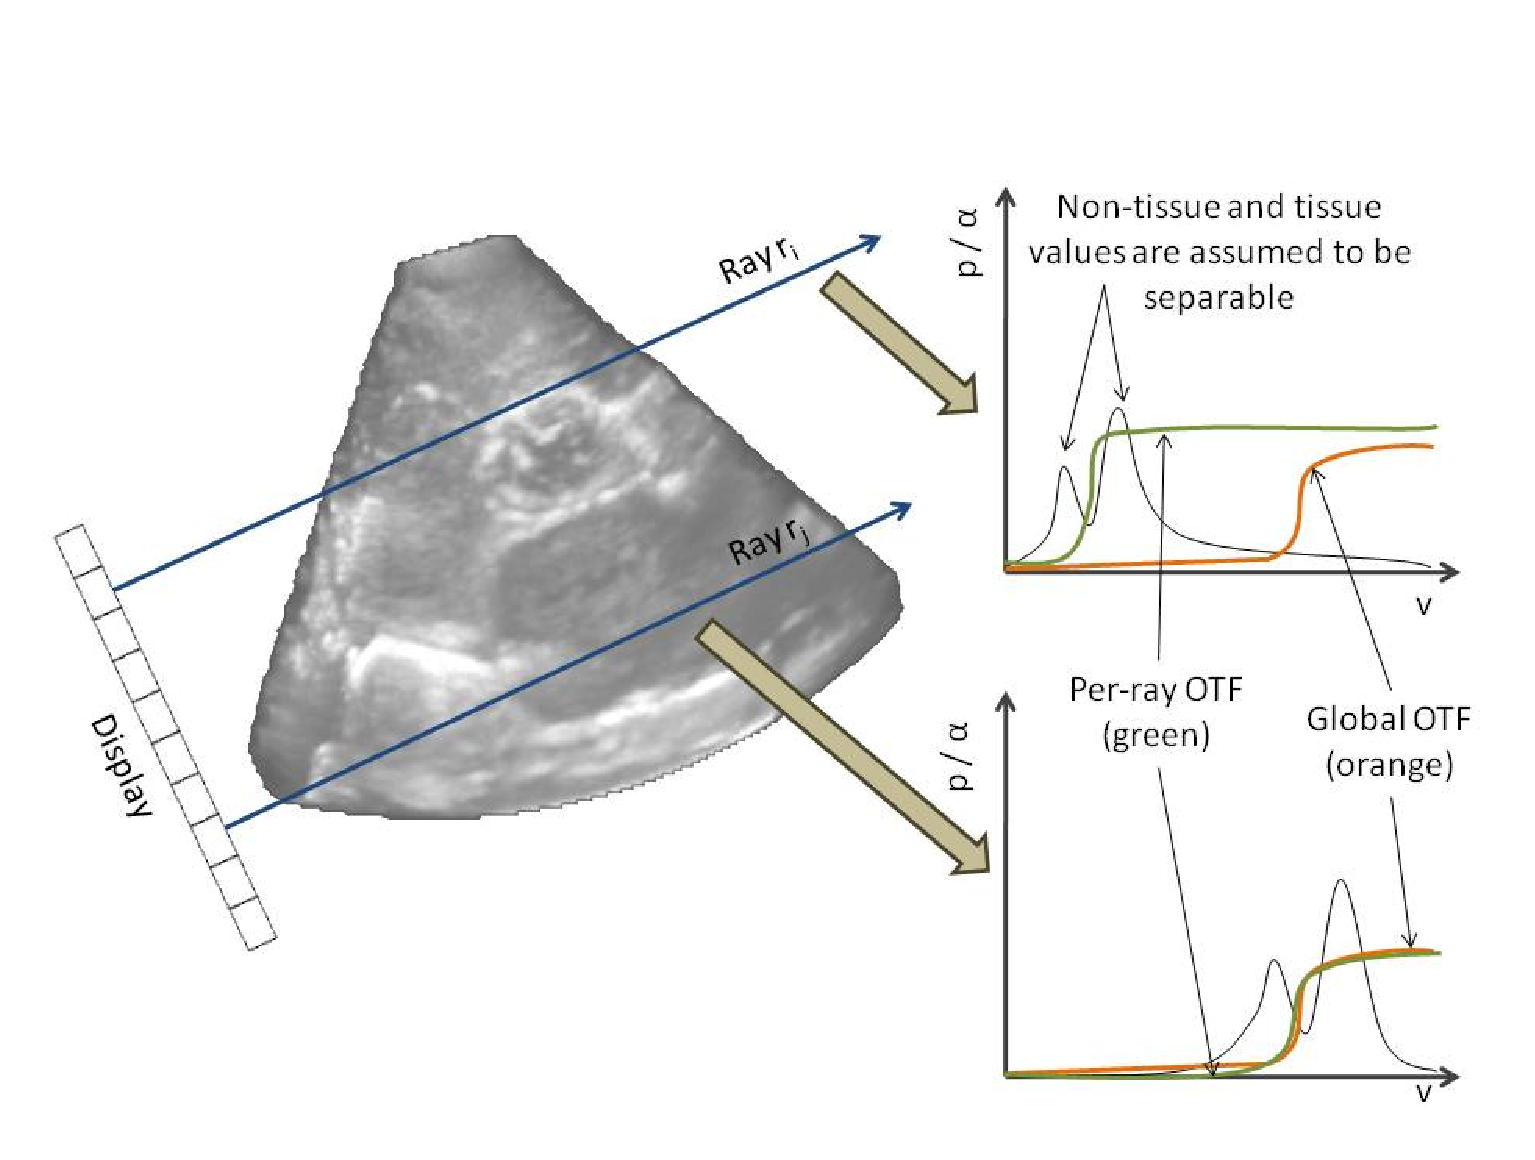
\includegraphics[height=0.52\textwidth]{lot.eps}\\ 
(a)\\
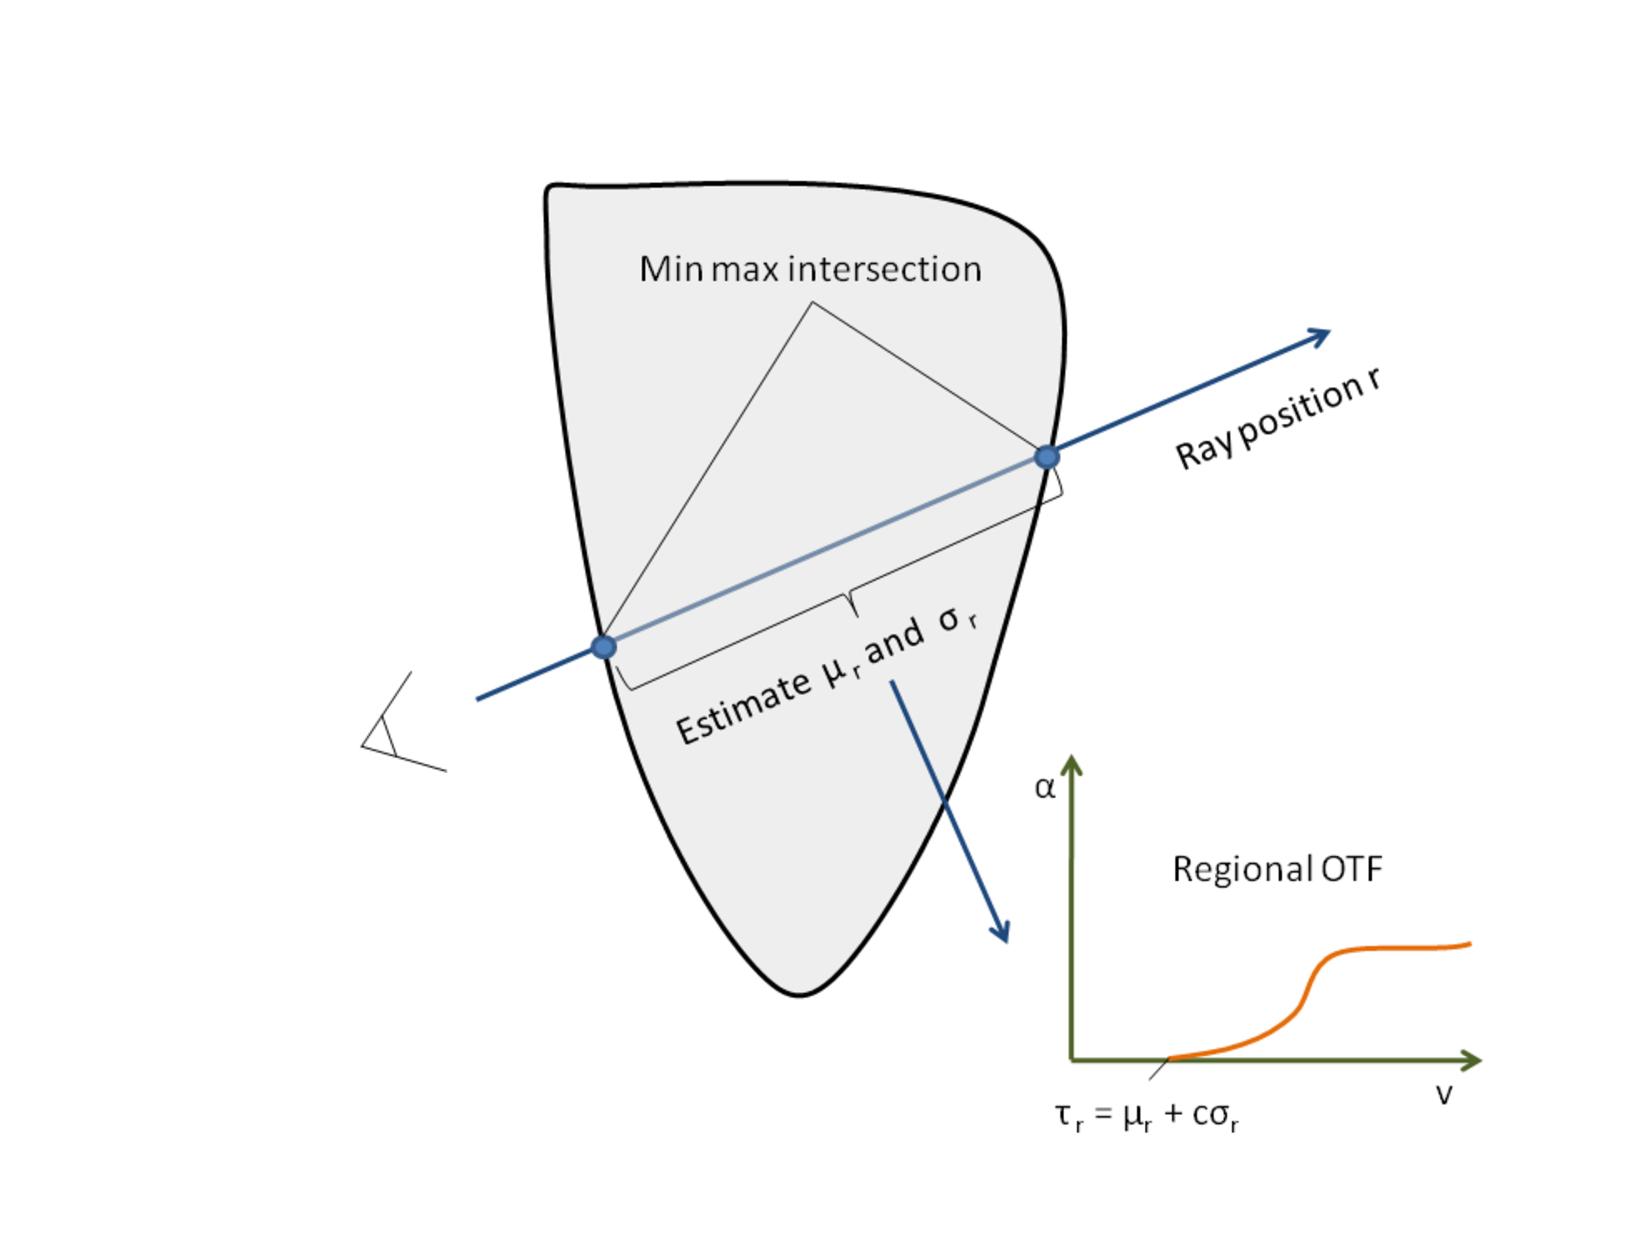
\includegraphics[height=0.52\textwidth]{lotf_mesh2.eps}\\
(b)
\end{tabular}
\end{center}
\caption[example] { \label{fig:lotf}  a) Shows ideal bimodal histograms of two density evolutions along ray $r_i$ and $r_j$. If we apply a global OTF (orange) on the given case we must select one ray were we want to separate tissue from blood. However, with a regional adapted OTF (green) we can find individual thresholds $\tau_r$ that minimizes the amount of misclassified samples along both rays. b) Estimated values of mean $\mu_r$ and standard deviation $\sigma_r$ inside the blood pool are used to regionally adjust the OTF. The regional opacity threshold $\tau_r = \mu_r + c\sigma_r$ is calculated for each ray $r$ intersecting a given left ventricular delineation.}
\end{figure} 
Since the global distributions of tissue and blood pool voxels usually overlap, adjusting $\tau$ will always involve a tradeoff between 
the number of true-positive and false-positive tissue voxels. If the opacity threshold is set too high, tissue surfaces will start to fall apart. However, if set too low, low level noise will get high opacity and the rendering will end before the actual tissue border is reached. Figure \ref{fig:lotf}a depicts the problem of having a global OTF (in orange). If rays $r_i$ and $r_j$ have noise ($n_r$) and tissue ($s_r$) levels given by $n_i$, $s_i$, $n_j$, $s_j$, with $n_i < s_i < n_j < s_j$, there are two obvious choices for $\tau$. The global opacity threshold $\tau$ can be selected as $n_i < \tau < s_i$ or $n_j < \tau < s_j$. The first choice makes $n_j$ occlude $s_j$, however the second choice will render $s_i$ transparent. This will result in an artificial hole in the final rendering along $r_i$. With our regional adaptive OTF, the idea is to let the opacity threshold $\tau$ vary across the framebuffer, making us able to define individual opacity thresholds for $r_i$ and $r_j$ (shown in green in Figure \ref{fig:lotf}a). 

In optical character recognition there has been a long tradition to utilize adaptive thresholding schemes to deal with variable background levels in 2D images\cite{Niblack1985}, thus maximizing the amount of foreground output. One simple adaptive method is based on estimates of regional statistics. The local image threshold $\tau_{x,y}$ is calculated as
\begin{equation}
\tau_{x,y} = \mu_{x,y} + c\sigma_{x,y},
\label{eq:niblack}
\end{equation}
where $c$ is a constant, and $\mu_{x,y}$ and $\sigma_{x,y}$ are mean and standard deviation estimates calculated in a window $w$ around (x,y). This yields what is known as a thresholding surface, where the method assumes that the foreground has higher expected value than the background inside $w$. Hence, foreground pixels are located above the thresholding surface.
	
To address our problem with high variability in tissue intensity in ultrasound images, we have designed a regional adaptive OTF by estimating the regional means and standard deviations of Equation \ref{eq:niblack} from the blood pool of the LV. The blood pool was delineated by a state-estimation algorithm capable of tracking the LV endocardium in real-time\cite{orderud2006}. The temporal state of the LV is returned by the framework as a time series of polygon meshes. How we utilize this information to do regional opacity adjustments is depicted in Figure \ref{fig:lotf}b. For a given frame we estimate the signal mean and standard deviation, $\mu_r$ and $\sigma_r$, along rendering ray $r$. Note that only the blood pool, the intersection between $r$ and the given LV delineation, is used to estimate $\mu_r$ and $\sigma_r$. The estimates are then used to calculate a regional opacity threshold $\tau_r$ given as
\begin{equation}
\tau_r=\mu_r+c\sigma_r, 
\label{eq:niblack_ray}
\end{equation}
where $c$ is a global constant adjusting $\tau_r$ around $\mu_r$ with a certain number of standard deviations. The local threshold $\tau_r$ together with Equation \ref{eq:otf} form our blood pool based regional adaptive OTF. Rays that do not intersect the given LV delineation are rendered using a global OTF.  


\subsection{Parameter space}
The proposed method in Equation \ref{eq:niblack_ray} introduces a parameter $c$, which controls how many standard deviations we want $\tau_r$ to deviate from the per-ray blood pool mean $\mu_r$. This parameter is clearly a substitution for the global opacity threshold, and adjusting $c$ will in the same way control the level of data visible in the rendered image. Setting $c = 0$ will render approximately $50\%$ of the blood pool samples transparent. Since we have a robust estimate of blood pool statistics, tissue signals are expected to have $\mu_{tissue} > \mu_r$ and $c > 0$ should be used.

The shape of the OTF is of great importance for the final appearance of a volume rendering. An OTF with a gentle slope will for instance result in a transparent look. In the proposed method we are more interested in the opacity threshold than the actual shape of the OTF, therefore we use the simple shifted and truncated second degree polynomial from Equation \ref{eq:otf} as a basis for the local OTF. Because it is a simple closed form expression, it can be used to quickly calculate on-the-fly opacity values.

For thresholding 2D images, the adaptive method in Equation \ref{eq:niblack} requires a window size that is directly related to the size of foreground objects. In our method, this window size depends on the ray-blood-pool intersection, and ideally no foreground (tissue) is included in the estimates. The regional opacity threshold $\tau_r$ is used along the full length of $r$, not just the intersection. Intersections with too few samples to give reliable statistics are rendered using a global OTF. 

\subsection{Spatial and temporal regularization}
Introducing adaptive visualization has some negative side effects. We trade spatial and temporal coherence in the presentation of anatomical structures for a better presentation of endocardial tissue. This does not pose any problems as long as the structure of interest along a given ray is associated with a value larger than the blood pool mean. Otherwise we risk rendering this structure transparent.
%The challenging part of estimating per-voxel relevance indicators in ultrasound data is to maintain spatial and temporal coherence of anatomical structures. 
%Since relevance in our method is proportional to intensity, structures of interest can be suppressed if they are not associated with a value larger than the blood pool estimate. 
The latter situation will often arise if e.g. the endocardium, mitral valve or papillary muscles are included in the estimated statistics. Given the properties of the real-time tracking framework, the two last structures, will to some extent, always be included. To exclude the endocardium we highly depend on a successful LV endocardial tracking. All segmentation algorithms will  be prone to errors and two regularization schemes have therefore been tested. First, we do spatial smoothing of estimates across neighbouring rays. This will constrain the regional adaptivity. Second, we do temporal smoothing over successive frames to reduce the per-frame adaptivity and potential flickering\cite{Peterscha2005}. The smoothing has been implemented as averaging filters on the framebuffer containing regional statistics. All regional adaptive renderings and statistics have been produced without any regularization in this paper. However the regularization schemes have been tested, and we will comment on how they perform.

%For each recording, a polygon model tracking the left ventricle has been provided by the AutoLVQ tool from GE Vingmed Ultrasound. With this information available, estimation of $\mu_r$ and $\sigma_r$ can be restricted to blood pool samples only. For rays intersecting the model, the opacity threshold $\tau_r$ is therefore a weighted sum between first and second order blood pool statistics along the ray. Other parts of the volume can be rendered using a global OTF.

\subsection{Rendering setup}
All renderings have been produced with Phong lighting and the data have been pre-smoothed with anisotropic diffusion\cite{perona1990scale, Steen}. %As common for 3D echocardiography, volume renderings are depth encoded for enhanced depth perception. 
For ray-casting it is normal to stop integrating when no significant transparency is left (known as early-ray-termination). We have chosen to terminate each ray when only $5 \%$ transparency is left. The rendering resolution has been set to 512x512x100.

\subsection{Measuring rendering accuracy}
As a measure of rendering accuracy, we have calculated the mean absolute error (MAE) between the rendering depth buffer (given by early-ray-termination) and a validated left ventrical segmentation. The reference segmentation was performed by an experienced physician echocardiographer using the AutoLVQ tool from GE Vingmed Ultrasound. The MAE measure will increase if the rendering contains tissue dropouts, or if spurious structures occlude endocardial tissue. A minimal MAE therefore exists when a majority of rays end their traversal near the tissue-blood border depicted by the reference segmentation. A view-aligned clipping plane has been applied to produce standard long-axis and mitral valve views, clipping away half of both the ventricle and the reference segmentation. Clipping of the volume from behind has also been applied to reduce the impact of non-terminated rays versus rays terminated by clutter noise.

\section{Results}\label{sec:res}

\subsection{Quantitative evaluation}
% table showing statistics
\begin{table}
\begin{center}
\begin{tabular}{c|ccc}
& Apical 4-chamber & Inverted apical 4-chamber & Mitral valve \\ \hline \\[-1.5ex]
$\bar{d}$ & $1.5 \pm 0.3$ mm & $2.5 \pm 0.4$ mm & $1.7 \pm 0.2$ mm\\ 
\end{tabular}
\end{center}
\caption[]{\label{tab:stat1} Statistics showing a significant improvement ($p < 0.001$, $\textrm{d.f.} = 17$) in mean absolute error (MAE) for the proposed regional adaptive method in three views. The variable $\bar{d}$ is the average difference plus-minus standard error between $\textrm{MAE}_{global}$ and $\textrm{MAE}_{regional}$ in 18 subjects.
%The null hypothesis that $\bar{d}$ is less than or equal to zero, i.e. $\textrm{MAE}_{global} \le \textrm{MAE}_{regional}$, has probability $p < 0.001$ for all views using t-statistics with $\textrm{d.f.} = 17$. 
All renderings are from end-diastole and were tuned to the best visual appearance by a physician echocardiographer.}
\end{table}
The global and regional adaptive methods were compared using a dataset of apical recordings from 18 subjects. The dataset consisted of 8 healthy volunteers and 10 subjects with recent myocardial infarctions and were acquired using the GE Vivid 7 Dimensions system (GE Vingmed, Horten, Norway) and a 2.5MHz matrix array transducer (GE Vingmed, Horten, Norway), with the subjects in the left lateral decubitus position. Scans were taken from the apical imaging
window, in harmonic mode, from 4 up to 6 QRS triggered sub-volumes, during an end-expiratory breath-hold. The depth and angle of the ultrasound sector were adjusted such that the entire LV was covered.

For each recording, three renderings from standard views (apical 4-chamber (A4C), inverted A4C and mitral valve (MV)) were generated for both the global and regional adaptive methods. Each rendering was then tuned to the best visual appearance by a physician echocardiographer. For each rendering we measured the MAE between the rendering depth buffer and a validated LV segmentation. The results of these measurements are reported in Table \ref{tab:stat1}. The null hypothesis that $\bar{d}$ is less than or equal to zero, i.e. $\textrm{MAE}_{global} \le \textrm{MAE}_{regional}$, can be rejected ($p < 0.001$) for all views using t-statistics with $\textrm{d.f.} = 17$.

The algorithm has been implemented on a GPU using CUDA. It runs at an average speed of 16 fps with an Nvidia GTX 460 graphics card. Note that this card has half the texture performance in CUDA compared to Direct3D. To estimate statistics we need to add a second pass through the volume to the rendering pipeline, reducing performance from 26 fps for a global OTF to 16 fps. As mentioned the rendering resolution is 512x512x100.

\subsection{Qualitative evaluation}
\begin{table}
\begin{center}
\begin{tabular}{c|ccc}
& Apical 4-chamber & Inverted apical 4-chamber & Mitral valve \\ \hline \\[-1.5ex]
Better & 17 & 17 &  12 \\ 
Equal  & 1 & 1 & 4\\
Worse & 0 & 0 & 2\\
\end{tabular}
\end{center}
\caption[]{\label{tab:stat2} Ratings given  by an experienced physician echocardiographer when comparing the blood pool based regional adaptive OTF with a global OTF in three views.}
\end{table}
For each pair of renderings, an experienced physician echocardiographer was asked to answer the following questions regarding image quality: \emph{Does the blood pool based regional adaptive OTF produce a rendered image with less tissue dropouts and spurious structures inside the blood pool compared with the global OTF?}. This qualitative evaluation is summarized in Table \ref{tab:stat2}. As seen, he concluded that the regional adaptive method performed better in 46 of the 56 renderings, and only worse in two.

\subsection{Examples}
% one figure showing some renderings
\begin{figure}  
\begin{center}
\begin{tabular}{cc}
\includegraphics[height=0.4\textwidth]{global_otf_cn02_crown.eps} & 
\includegraphics[height=0.4\textwidth]{global_otf_crown.pdf}\\
(a) & (b)\\
\includegraphics[height=0.4\textwidth]{regional_otf_c05_crown.pdf} & 
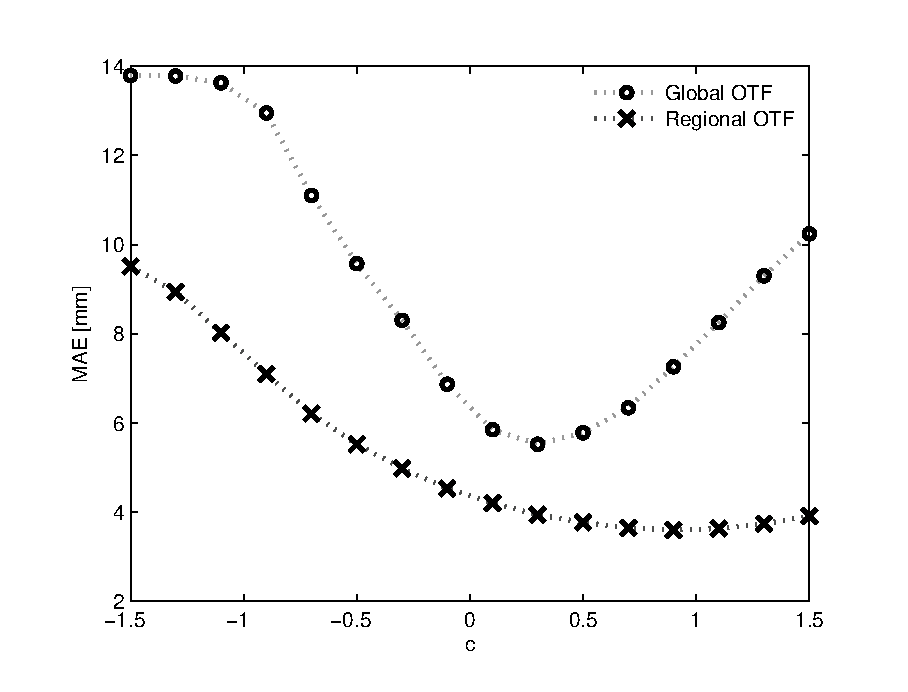
\includegraphics[height=0.4\textwidth]{residualGraphVsC.eps}\\
(c) & (d)
\end{tabular}
\end{center}
\caption[example] { \label{fig:vis} a) Global OTF with a low opacity threshold $\tau$. A lot of noise is visible inside the LV (circle). b) Global OTF with $\tau$ corresponding to the lowest MAE in Figure d. The image contains less noise, but also a large tissue dropout (circle). c) Blood pool based regional adaptive OTF with c=0.5 which is close to the minimum in d. The papillary muscle is now more visible (arrow) and the tissue dropout (circle) is smaller without pruning the mitral valve (sqare).  d) Parameter exploration in the view shown in a, b and c. MAE is plotted versus the $c$-value. For comparison, the global OTF has been converted into a function of $c$ using the global mean and standard deviation.}
\end{figure} 

Figures \ref{fig:vis}a, b and c show three renderings of the same apical 4-chamber view of one subject. With a low opacity threshold (Figure \ref{fig:vis}a), a lot of clutter noise is picked up in the apex of the LV (circle). With a threshold corresponding to the minimum MAE in Figure \ref{fig:vis}d, the clutter noise is removed (Figure \ref{fig:vis}b), but a tissue dropout (circle) has now increased in size. With the blood-pool based method (Figure \ref{fig:vis}c) clutter noise inside the LV is suppressed, giving a clear view of the endocardial tissue and a papillary muscle (arrow) without reducing the thickness of the mitral valve (square). The extent of the mentioned dropout is also reduced (circle). In Figure \ref{fig:vis}d we present a parameter exploration of the $c$-value introduced with the regional adaptive OTF. For comparison the global opacity threshold is substituted with a function of $c$, global mean and standard deviation. The figure shows that for a given view the MAE measure has a local minimum for both the global and regional methods, and that the regional OTF has a smaller MAE than the global OTF for all $c$.

% show spatial regularization

\section{Discussion}
% summarising contribution
A regional adaptive OTF based on blood-pool statistics has been proposed. The purpose was to better handle the high variation of signal within tissue as well as variability of noise signal inside the blood pool. Both quantitative and qualitative results reported in Section \ref{sec:res} shows that this has been accomplished. 

% Discuss quantitative results
We believe that the significant reduction in MAE for the regional adaptive method in Table \ref{tab:stat1} is caused by a reduced amount of rendering outliers. By outliers we mean rendering rays that stop far away from the endocardial boundary depicted by the reference segmentation, thus having a high absolute error. We observe that the difference in MAE in millimetre is small, between 1.5 and 2.5 mm for the three views in Table \ref{tab:stat1}, compared to normal average end-diastole myocardial thickness (around 10mm). However, regional improvements in order of centimetres can be observed in Figure \ref{fig:vis}c (circle). These large improvements are smoothed out by the MAE measure, but remains as a significant statistical improvement ($p<0.001$) in MAE-difference between the regional and global adaptive method in all three views (Table \ref{tab:stat1}).

% Discuss qualitative results
Table \ref{tab:stat2} shows that in 46 pair of renderings the regional adaptive OTF based on blood pool statistics provided renderings with less tissue dropouts and spurious structures inside the blood pool. However, Table \ref{tab:stat2} also shows that the regional adaptive method was ranked worse in the MV view for two subjects, and in four MV-views the two methods were equal. On the other hand, the MV statistics in Table \ref{tab:stat1} are the most significant among the three views. One explanation to these diverging results is: When doing the qualitative assessment the physician echocardiographer watched the whole cardiac cycle, where the statistics in Table \ref{tab:stat1} are calculated from a single end-diastolic frame. In end-diastole the mitral valve is closed, which means that the MV is outside our tracking model and therefore not included in the blood pool statistics. When the MV is inside the tracking model, thus included in the estimates, visual artefacts can occur since the MV will be treated as being a part of the blood pool and might get rendered transparent. %It is important to prevent this, given the high clinical value that the MV represent. 
Another explanation is that all the recordings are from an apical imaging view. From this view the MV is normal to the ultrasound beam. The MV has because of this better image quality than e.g. the LV endocardium and thus less variation is observed in the MV-view statistics than for the long-axis views (Table \ref{tab:stat1}). When the image quality is good it is hard to make any regional improvement compared with a global OTF. Opposite, the endocardial boundary has usually lower image quality than the MV from the apical imaging window. For the two 4-chamber views the statistics therefore has higher variation and for the inverted 4-chamber, that had large acoustic dropouts in many of the recordings, the improvement is much larger. 

% Discuss example renderings
The images in Figure \ref{fig:vis} demonstrate that our regional adaptation of the OTF provides a better tradoff between artificial tissue dropouts and spurious structures compared with a global OTF. In Figure \ref{fig:vis}d this improvement is quantified as $\textrm{MAE}_{global}(c) > \textrm{MAE}_{regional}(c), \forall c\in[-1.5, 1.5]$. This illustrate our findings that the global OTF did not produce a smaller MAE than the regional OTF in any pair of renderings if both methods where tuned to the lowest MAE. The gentle slope of $\textrm{MAE}_{regional}(c)$ in Figure \ref{fig:vis}d is another important observation. This indicates that the proposed method is less sensitive to changes in c, and therefore less tuning is often required. This observation was also done by the physician echocardiographer. 
The rendering in Figure \ref{fig:vis}c has a c-value corresponding to the minimum of $\textrm{MAE}_{regional}(c)$ in Figure \ref{fig:vis}d. We have often found the c-value at the local minimum of the MAE measure to be approximately the same c-value as both we and the physician echocradiographer would have selected in a given view. A fully automatic method could therefore iterate towards the local minimum by steepest descent, removing the need for manual tuning of $c$. It should be kept in mind that the success of this approach highly depends on a correct segmentation of the LV. This approach will also not be real-time, since an accurate segmentation of the LV usually involves manual adjustments and processing times in the order of seconds. One option is to use the real-time acquired LV delineation, used to estimate blood pool statistics, to measure rendering accuracy as well. A different endocardial detection scheme should then be used to estimate blood-pool statistics, to avoid a too close coupling between the LV delineation used for estimation and validation. 

%Discuss spatial and temporal smoothing
As mentioned, no spatial regularization was applied to the results in Section \ref{sec:res}. However, spatial smoothing will decrease the variation in $\tau_r$ across the image, and with increased filter kernels the results will become equivalent to applying an OTF with a global adaptive opacity threshold $\tau_g$ based on the whole blood pool. With increased spatial smoothing less visual artefacts have been observed at the cost of a higher MAE. As no flickering has been observed, temporal smoothing had no positive effect. E.g. the rapid movement of the mitral valve caused artificial dropouts in all views when temporal smoothing was applied. 

\subsection{Limitations}
The choice of using a deformable model to indicate the blood pool location imposes some limitations for the proposed method. As mentioned, some important cardiac structures are included in the depicted blood pool and might result in visual artefacts. However, how the LV endocardial boundary is derived is not relevant for the result in this paper. Local edge detectors combined with regularization may work equally well for limiting the regional estimation of means and standard deviations to the blood pool.


%Caused by the decision of using a deformable model to indicate the blood-pool location.

\section{Conclusion}
%Many adaptive algorithms for DVR have been proposed in the literature, however they are usually tested on data with considerably higher SNR than ultrasound. We have proposed a method for fast adaptive visualization of low-SNR cardiac 3D ultrasound. Compared with a global OTF we have shown that the regional adaptive method, based on blood pool statistics, is capable of providing a better tradeoff between tissue dropouts and the number of spurious structures inside the blood pool. The need for manual tuning is reduced by adapting the OTF to the data at hand, potentially leading to a fully automatic, data-dependent OTF.
In this paper we have introduced and investigated an adaptive DVR method for real-time visualization of cardiac 3D ultrasound. Compared to a global OTF we have shown, both with quantitative and qualitative results, that the regional adaptive method, based on blood pool statistics, is capable of reducing tissue dropouts and spurious structures inside the blood pool. The need for manual tuning is reduced by adapting the OTF to the data at hand, potentially leading to a fully automatic and data-dependent OTF.

\newpage\addcontentsline{toc}{section}{References}
\putbib[./Paper4/spiebib]
\end{bibunit}

%%%% Paper 5 %%%%
\begin{bibunit}[IEEEtran]
\CustChapterPaper{Huygens on Speed: Interactive Simulation of Ultrasound Pressure Fields}
\runningtitle{Huygens on speed}
\authors{\textbf{Jon Petter \AA{}sen}$^1$ and Sverre Holm$^{1,2}$}
{
	$^{1}$Medical Imaging Lab (MI-Lab), Norwegian University of Science and Technology, Trondheim, Norway\\
    	$^{2}$Department of Informatics, University of Oslo, Oslo, Norway
}
\noindent \textit{Proc. IEEE Ultrasonics Symposium 2012, pp. 1643-1646}.
\newpage\graphicspath{{./Paper5/}}

\begin{abstract}
The introduction of graphics processing unit (GPU) computing has made it possible to speed up computationally demanding algorithms. One of these algorithms is the calculation of pressure fields from acoustic transducers. Here, the execution time often limits the number of elements and field points we can select in order to get results back in finite time. 

In this paper we present a simple GPU-based simulator capable of simulating high resolution pressure fields at interactive frame rates. The simulator is based on the same principle as the Ultrasim toolbox, where responses from several point sources are accumulated in a set of observation points, hence solving the Rayleigh-Sommerfeld integral. The cumulative sum for each observation point is independent of all other observation points, making the problem perfect for GPU processing. For the simulator we provide both a Paint-like interface for interactive drawing of uniform linear arrays and free-hand shapes, and a Matlab interface for precise scripting of element positions and observation points.

The presented GPU simulator was compared both with a multi threaded C-version, Ultrasim, and Field II. Compared with Ultrasim we report a 400 times speedup when simulating a varying number of source points on a 150 K points observation grid. The test system consisted of a low-end GPU (Nvidia Quadro 600) and an Intel i7-870 2.93 GHz quad-core CPU.

\end{abstract}

\section{Introduction}
Software for simulation of pressure fields from ultrasound transducers is an important tool for gaining knowledge on how a transducer performs. This brings both great insight to researchers and helps lowering production costs. A downside is that calculating large fields is often found to be time consuming, and the number of field points and the level of transducer approximation have to be adjusted low enough to have the result back in finite time. The introduction of graphics processing unit (GPU) computing has made it possible to speed up computationally demanding algorithms. In this paper we present a simple GPU-based simulator capable of simulating high resolution pressure fields at interactive frame rates.

Today there exist a vast collection of ultrasound simulators. There is Field II by Jensen\cite{Jensen1992}, considered the gold standard of ultrasound simulation. However, there are also simulators that provides different functionality and perform different trade-offs than Field II. One example is the Ultrasim toolbox\cite{Holm2001}. As for Field II, this is also a Matlab plugin. However, where Field II is mostly used to simulate ultrasound images and beams, Ultrasim can only simulate snapshots of transducer transmit fields. Another difference, is the way these toolboxes are organized. Field II is a collection of functions that makes it easy to run large batched simulations where different acquisition setups are to be investigated. Ultrasim, on the other hand, is an interactive tool with a graphical user interface controlling all simulation parameters. Ultrasim is therefore more accessible if one only need to simulate transducer transmit pressure. Field II and Ultrasim are based on two different concepts, the spatial impulse response and Huygens' principle respectively. In addition there are also simulators based on the angular spectrum method \cite{Prieur2012} capable of simulating 3D harmonic fields. And lately, simulators, capable of simulating 3D ultrasound images in orders of seconds have also been introduced \cite{Hergum2009}.

\begin{figure}[!t]
\centering
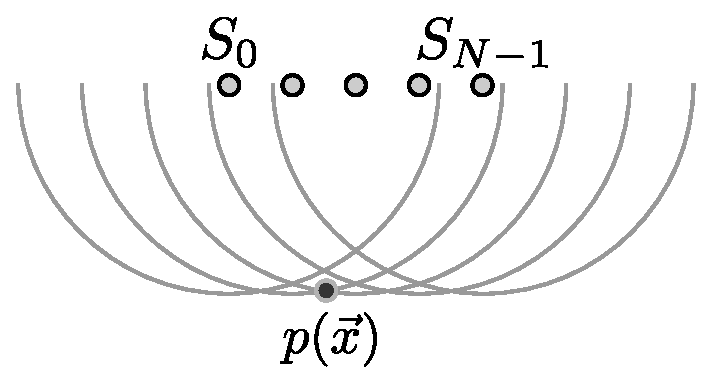
\includegraphics[width=3in]{img/huygens_principle.eps}
\caption{Huygens' principle showing the superposition of spherical waves from many point sources.}
%Huygens' principle. A wave front, here represented by the diffraction pattern formed by a narrow slit, can be represented as the superposition of spherical waves originating from an infinite set of point sources placed inside the opening. If we limit the calculation to a finite set of source points  $\{S_i\}_{i=0}^{N-1}$, field pressure, $p$,  at a given location $\vec{x}$, can be found as the coherent sum of the $N$ contributing sources.}
\label{fig:huygens_principle}
\end{figure}

Like Ultrasim, the presented simulator, Huygens on Speed (HOS), is based on Huygens' principle \cite{huygens} as depicted in Fig. \ref{fig:huygens_principle}. Hence, solving the Rayleight-Sommerfeld integral\cite{Holm2001}:
\begin{equation}
\phi = \frac{1}{2\pi} \int_S \frac{u_n(r_0, t-r/c)}{r}dS.
\end{equation}
where $u_n$, the normal velocity, is integrated over the transducer surface $S$ weighted with the reciprocal of distance from the field point to the transducer.

We easily see that each calculation at a given field point is independent of the result at all other field points. The problem is therefore perfect for GPU computing, since one thread on the GPU can process one field point independent of all other threads. The only inputs needed are the field point and source point properties. Examples of other simulators implemented using GPU computing includes \cite{Hlawitschka2010} and \cite{Gjerald2012}. The first simulates 3D pressure fields at high speeds using a fast near field method, and the latter is capable of simulating ultrasound images in real time using convolution and an assumption of a shift-invariant imaging system.

The simulator presented in this paper is designed to be an interactive tool for drawing and exploring different array geometries.  It is our belief that the simulator can be used both in research and academic teaching, as a neat way of demonstrating array beamforming principles.

%Methods for calculating pressure from rectangular pistons \cite{Mast2007, McGough2004}.

\section{Method}\label{sec:method}

The presented simulator works by discretizing the surface $S$ found in the Rayleigh-Sommerfeld integral into a set of point sources, $\{S_i\}_{i=0}^{N-1}$. As shown in Fig \ref{fig:huygens_principle}, the total field pressure, $p$, at position $\vec{x}$ can then be found as the coherent sum of $N$ monochromatic spherical waves:
\begin{equation}\label{eq:sum}
p(\vec{x}) = \sum_{i=0}^{N-1} \frac{A_i}{r_i}e^{2 \pi j f_i t_i}.
\end{equation}
Here, $A_i$ is the source amplitude or apodization, $f_i$ is the source frequency, $r_i$ is the distance from $\vec{x}$ to $S_i$, and $t_i$ is the wave travelling time given by $t_i = r_i/c - t + t_{S_i} + \Delta_i$, where $c$ is the speed of sound, $t$ is the snap shot time stamp, $t_{S_i}$ is the source time stamp, and $\Delta_i$ is the steering and focusing delay. Hence, a simple simulator based on (\ref{eq:sum}) works by rendering the contribution from a set of point sources with their corresponding properties in a set of observation points. How the source and observation points are positioned and what they represent is left for the user to decide. 

\section{Design}
\begin{figure*}[!t]
\centering
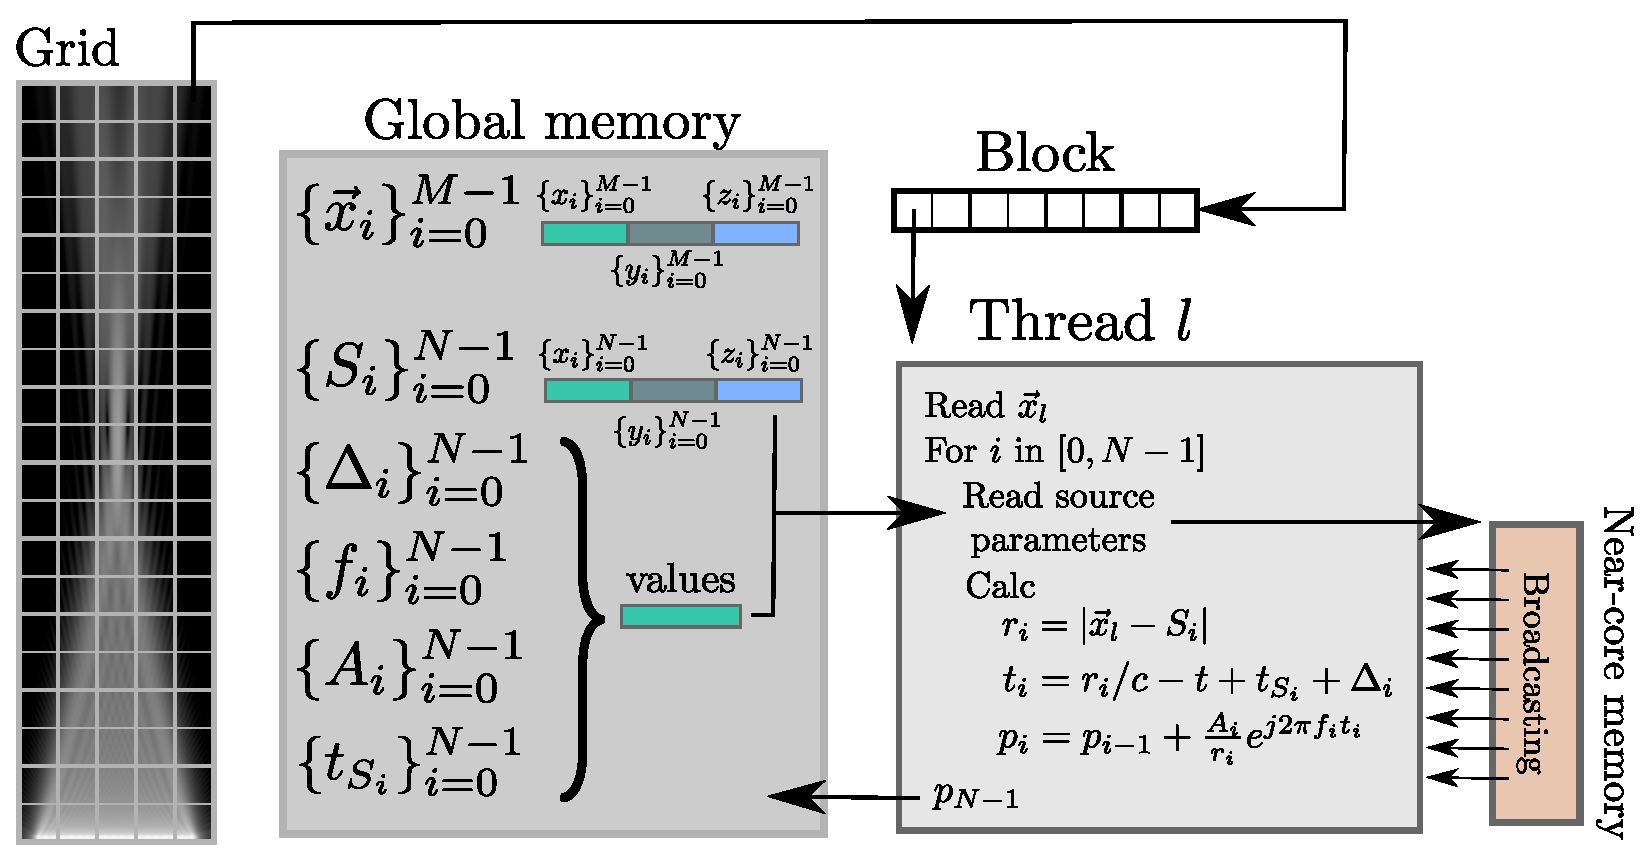
\includegraphics[width=\textwidth]{img/huygens_gpu_layout.eps}
\caption{Implementation of Huygens' principle on the GPU. One thread is launched per observation point, here presented as an azimuth plane. Each thread then reads the corresponding observation point, and collaborates on loading source point properties to near-core memory. From near-core memory, source properties are broadcast to registers when the kernel iterates over the set of sources. Note the coalesced memory layout of $\vec{x}$ and $S$ in global memory. The figure reflects the notation used in Section \ref{sec:method}.}
\label{fig:huygens_gpu}
\end{figure*}

From (\ref{eq:sum}) we see that field energy at a given observation point, $\vec{x}$, can be found independently from all other locations in space, and just as important, the result for each observation point is written to different bits of memory. Such a problem is perfect considering the GPU's ability of processing hundreds of pixels/threads in parallel. The implementation of (\ref{eq:sum}) used in the presented simulator is depicted in Fig \ref{fig:huygens_gpu}. One thread is launched per observation point. The reason for using this level of granularity is that the number of observation points is usually large compare to the number of source points. We also end up with enough instructions per thread to hide memory and instruction latency. On the other hand, if we have more source points than observation points, we should parallelize across source points instead. However, the result from each source point has to be written to equal positions in memory, making barriers that would significantly lower the method's throughput. Continuing the discussion of Fig. \ref{fig:huygens_gpu}, the threads inside a given block work together to load all source points and their corresponding properties to near-core memory. Since all threads inside a block work on the same source simultaneously, we make use of broadcasting to feed one source to all threads in a single read per property. Note also how observation and source points are organized in global memory for coalesced reads, and by that maximizing global memory throughput.

As front-end to the presented simulator we provide both a Matlab scripting environment and a Paint-like user interface for interactive drawing of arrays and freehand shapes. The Matlab interface is minimal but highly flexible. The functional interface takes as arguments the values listed in global memory in Fig. \ref{fig:huygens_gpu}, and returns the calculated pressure for each observation point. Constructing and discretizing transducer arrays into points and calculating delays etc. is left for the user. However, an example script of how this could be done is provided. 

After increased speed, the main contributions in this work is how the user interface has been composed to make an interactive and interesting experience out of exploring acoustical arrays and their properties. The user interface works like a paint program, where point sources are added based on mouse interaction. There are several supported modes of interaction, and extensions to more advanced modes are obviously possible. However, when selecting modes of drawing, precision in source point positions have not been our focus. For that, one have the Matlab interface.  Supported modes include click-and-drag of $n\lambda$-spaced arrays and freehand drawing. For both these modes there exist both pulsed and continuous wave modes. 

In click-and-drag mode, equidistant point sources are created along a straight line from where the left mouse button was clicked to where it is released using the specified $\lambda$-spacing. The result is an array with one point source per element. Hence, there is no element directivity. In freehand drawing, a new point source is added for each mouse-moved event that occurs when the left mouse button is down, just like freehand drawing in Paint. 

After point sources have been added, they can all be focused in a common field point by right-click-and-drag. This can be used e.g. to illustrate how ultrasound arrays are able to sweep the beam in space, and how the beam can be focused at different depths. In pulsed-wave mode this can be used to illustrate how a pulse evolves when moving through the focus. Other concepts that can be interactively visualized both in pulsed and continuous wave mode include among other; frequency dependent resolution and depth of field, the effect of apodization, grating lobes and side lobes, near- and far-field transitions, and multiple focus zones.      


\begin{figure}[!t]
\centering
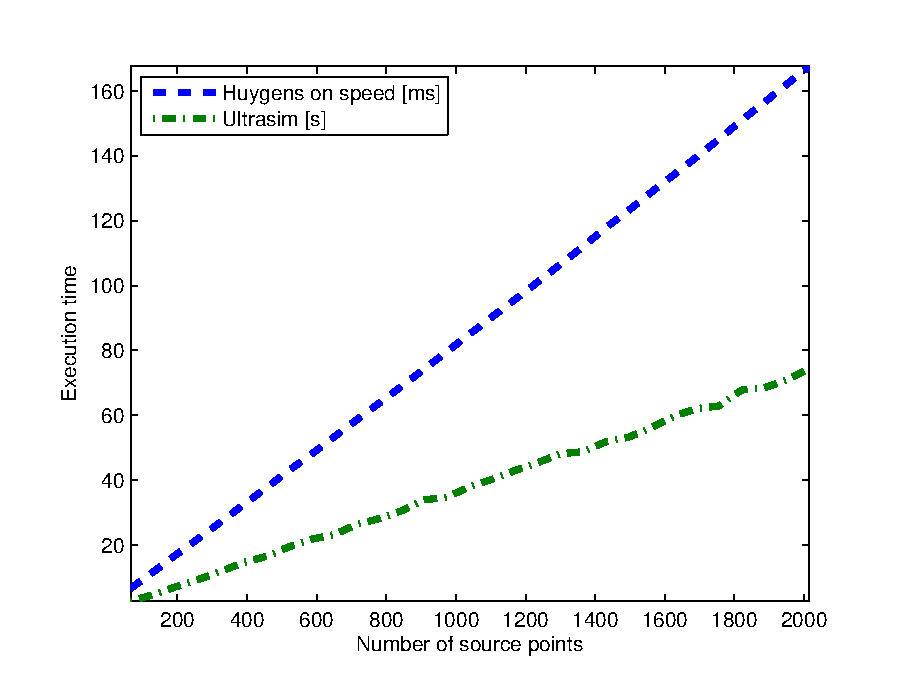
\includegraphics[width=0.8\textwidth]{img/hos_vs_ultrasim_plot.eps}
\caption{Benchmark of HOS and Ultrasim. Test setup consisted of 150 K observation points.Note that execution times for the presented simulator are in order of milliseconds whereas execution times for Ultrasim are reported in seconds. The target platform was a low-end Nvidia GPU (Quadro 600, 96 cores GPU) and a high-end Intel quad-core CPU (i7-870, 2.93 GHz).}
\label{fig:huygens_vs_ultrasim}
\end{figure}

\section{Results and Discussion}

\begin{figure*}[!t]
\centerline{
\subfloat[Lateral pressure]{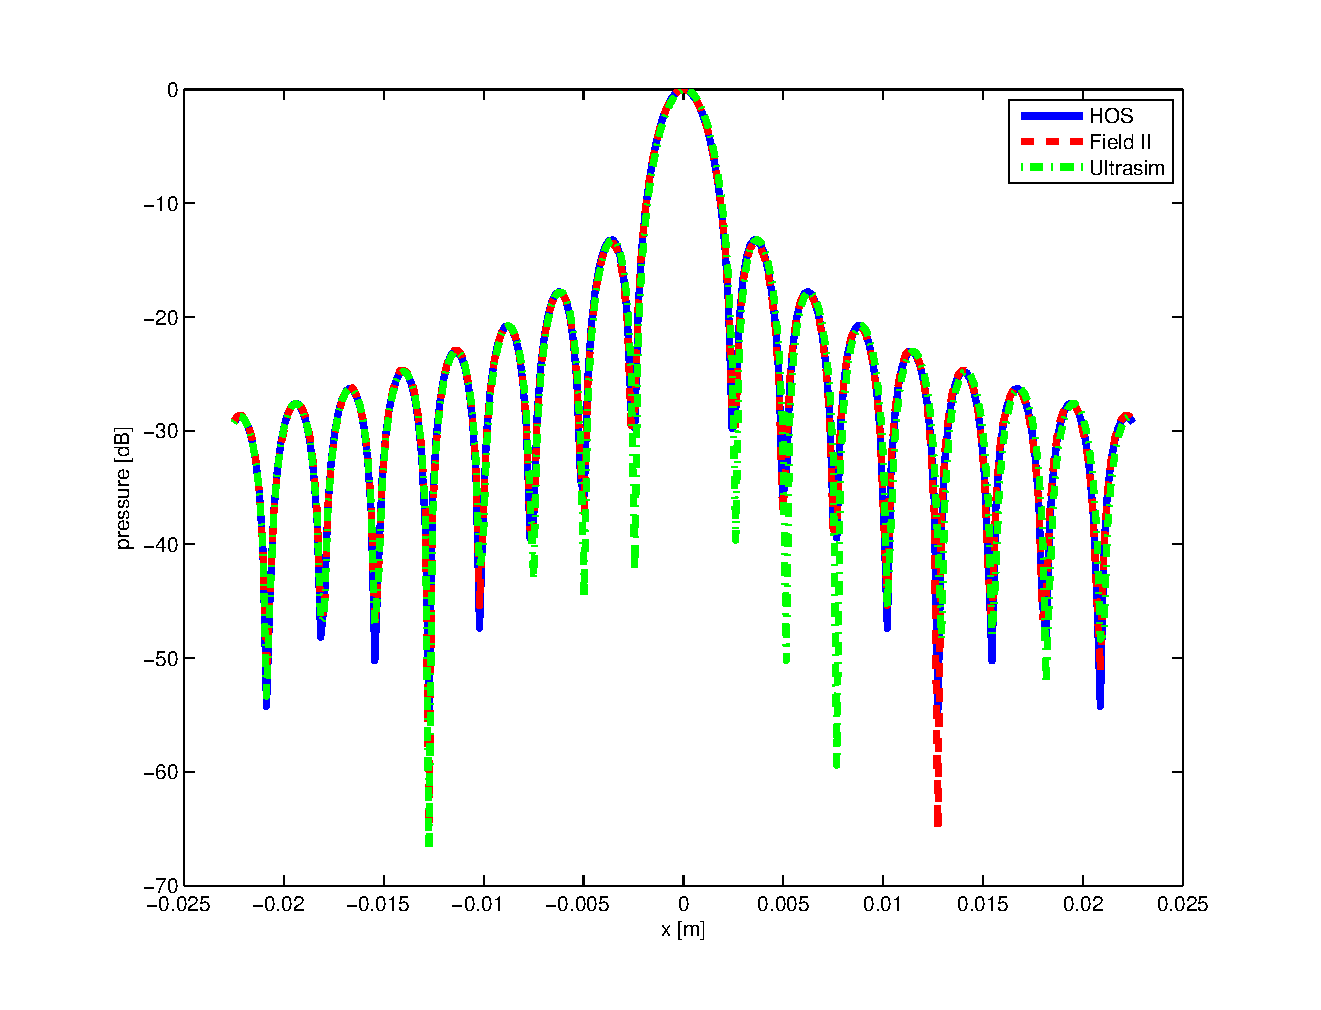
\includegraphics[width=0.5\textwidth]{img/hos_ultrasim_field_lateral.eps}\label{fig:lateral_pressure}}
\newline
\subfloat[Axial pressure]{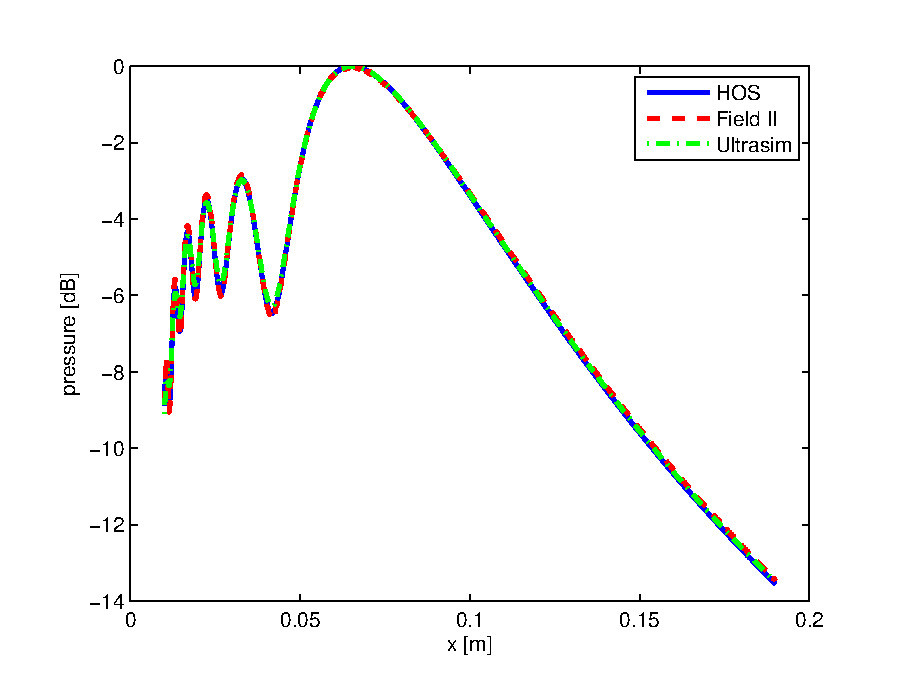
\includegraphics[width=0.5\textwidth]{img/compare_hos_field_usim2.eps}\label{fig:radial_pressure}}
}
\caption{Profiles of pressure generated by HOS, Ultrasim and Field II. The simulated array has 64 elements, a center frequency of 2.5 MHz, $\lambda/2$ pitch, and $\lambda/2$ wide and $10\lambda$ high elements. Uniform apodization is used and the array is focused at 8 cm depth. 5 source points (mathematical elements in Field II) were used in azimuth and 20 in elevation.}
\label{fig:huygens_vs_ultrasim_fieldII}
\end{figure*}

\begin{figure}[!t]
\centerline{
\subfloat[HOS]{\includegraphics[height=0.8\textwidth]{img/hos_pressure3.eps}\label{fig:hos_field}}
\subfloat[Ultrasim]{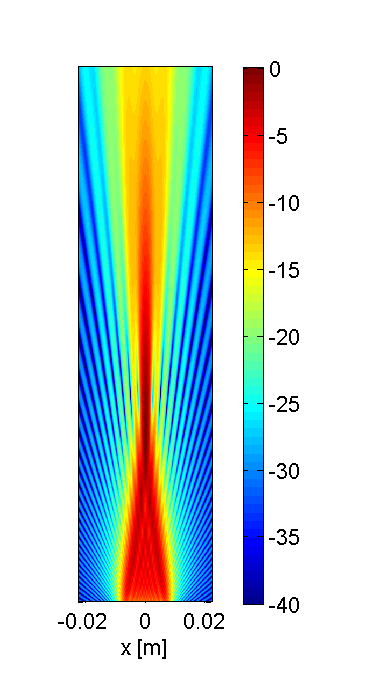
\includegraphics[height=0.8\textwidth]{img/ultrasim_pressure3.eps}\label{fig:ultrasim_field}}
}
\caption{Azimuth pressure field in dB generated by the presented simulator and Ultrasim for the same array simulated in Figure \ref{fig:huygens_vs_ultrasim_fieldII}. The resolution is 5.6 observation points per mm for both (250K observation points in total).}
\label{fig:huygens_vs_ultrasim_pressure_field}
\end{figure}

\begin{figure*}[!t]
\centering
\includegraphics[width=\textwidth]{img/freeHandDrawing2.png}
\caption{Free hand drawing of source points using the interactive user interface.}
\label{fig:huygens_free_hand}
\end{figure*}

Implementing Huygens' principle on the GPU results in a significant speedup, that again allows for interactive simulations of dense pressure fields from acoustical arrays. We show this in Fig. \ref{fig:huygens_vs_ultrasim} by presenting a benchmark made between HOS and Ultrasim. Note that execution times are reported in seconds for Ultrasim and milliseconds for HOS. Thus the average speedup is 400x in favour of HOS across the selected range of source points. 

Fig. \ref{fig:lateral_pressure} shows the in-focus (at 80mm) lateral pressure from a 2.5MHz, 64 element ($32\lambda$ wide and $10\lambda$ high, $5 \text{ azimuth} \times 20 \text{ elevation}$ points/subelements per aperture) uniform linear array calculated with HOS, Field II and Ultrasim. The beam profiles are strikingly similar. In Fig. \ref{fig:radial_pressure} we also see that all three simulators yield the same result along an axial cut through focus. The continuous pressure field calculated with Field II was found by taking the fourier transform of the total transmit beam energy at the center frequency. 
%Better element directivity might cause the focus offset using Field II compared with the other simulators.

Fig. \ref{fig:huygens_vs_ultrasim_pressure_field} shows the azimuth pressure field calculated using HOS (a) and Ultrasim (b). The resolution is 5.6 observation points per mm for both, hence 250K observation points in total. HOS and Ultrasim used 2 seconds and 3 minutes 40 seconds respectively in order to generate the image, hence a 110x speedup. The hardware used in this comparison was an Nvidia GT520, 48 cores GPU, and a i7-870 Intel quad-core CPU. A multi threaded C-version of the presented simulator used 1 minute and 45 seconds to generate the same image. Field II used 2 minutes 51 seconds. Note that Field II has to calculate the spatial impulse response for all observation points, and is therefore not directly comparable to Ultrasim's snap-shot-mode. The spatial impulse response can be calculated using HOS by iterating in time. Using the available low-end GPU and high-end CPU, the presented simulator and Field II are equally fast on this operation (without using streams on the GPU). However, for massive parallel calculation of the spatial impulse response one might want to apply a different parallelization scheme and level of granularity than what is described in this paper.

Fig. \ref{fig:huygens_free_hand} shows how arrays of any shape can be interactively drawn using the provided user interface. A video of how the interactive user interface works can be found at \cite{hos}.

% An example of a floating figure using the graphicx package.
% Note that \label must occur AFTER (or within) \caption.
% For figures, \caption should occur after the \includegraphics.
% Note that IEEEtran v1.7 and later has special internal code that
% is designed to preserve the operation of \label within \caption
% even when the captionsoff option is in effect. However, because
% of issues like this, it may be the safest practice to put all your
% \label just after \caption rather than within \caption{}.
%
% Reminder: the "draftcls" or "draftclsnofoot", not "draft", class
% option should be used if it is desired that the figures are to be
% displayed while in draft mode.
%
%\begin{figure}[!t]
%\centering
%\includegraphics[width=2.5in]{myfigure}
% where an .eps filename suffix will be assumed under latex, 
% and a .pdf suffix will be assumed for pdflatex; or what has been declared
% via \DeclareGraphicsExtensions.
%\caption{Simulation Results}
%\label{fig_sim}
%\end{figure}

% Note that IEEE typically puts floats only at the top, even when this
% results in a large percentage of a column being occupied by floats.


% An example of a double column floating figure using two subfigures.
% (The subfig.sty package must be loaded for this to work.)
% The subfigure \label commands are set within each subfloat command, the
% \label for the overall figure must come after \caption.
% \hfil must be used as a separator to get equal spacing.
% The subfigure.sty package works much the same way, except \subfigure is
% used instead of \subfloat.
%
%\begin{figure*}[!t]
%\centerline{\subfloat[Case I]\includegraphics[width=2.5in]{subfigcase1}%
%\label{fig_first_case}}
%\hfil
%\subfloat[Case II]{\includegraphics[width=2.5in]{subfigcase2}%
%\label{fig_second_case}}}
%\caption{Simulation results}
%\label{fig_sim}
%\end{figure*}
%
% Note that often IEEE papers with subfigures do not employ subfigure
% captions (using the optional argument to \subfloat), but instead will
% reference/describe all of them (a), (b), etc., within the main caption.


% An example of a floating table. Note that, for IEEE style tables, the 
% \caption command should come BEFORE the table. Table text will default to
% \footnotesize as IEEE normally uses this smaller font for tables.
% The \label must come after \caption as always.
%
%\begin{table}[!t]
%% increase table row spacing, adjust to taste
%\renewcommand{\arraystretch}{1.3}
% if using array.sty, it might be a good idea to tweak the value of
% \extrarowheight as needed to properly center the text within the cells
%\caption{An Example of a Table}
%\label{table_example}
%\centering
%% Some packages, such as MDW tools, offer better commands for making tables
%% than the plain LaTeX2e tabular which is used here.
%\begin{tabular}{|c||c|}
%\hline
%One & Two\\
%\hline
%Three & Four\\
%\hline
%\end{tabular}
%\end{table}


% Note that IEEE does not put floats in the very first column - or typically
% anywhere on the first page for that matter. Also, in-text middle ("here")
% positioning is not used. Most IEEE journals/conferences use top floats
% exclusively. Note that, LaTeX2e, unlike IEEE journals/conferences, places
% footnotes above bottom floats. This can be corrected via the \fnbelowfloat
% command of the stfloats package.



%\section{Conclusion}
%The conclusion goes here.




% conference papers do not normally have an appendix

The simulator can be downloaded from the same site \cite{hos}. The source code has been made available at github \cite{hosGit}. Contributions are welcome.

% use section* for acknowledgement
\section*{Acknowledgment}
The authors would like to thank Tore Bj\aa{}stad, Torbj\o{}rn Hergum and Hans Torp for the initial idea of creating the HOS simulator.



\newpage\addcontentsline{toc}{section}{References}
\putbib[./Paper5/hosbib]
\end{bibunit}

%\appendix

\end{document}
